% Alternative Options:
%	Paper Size: a4paper / a5paper / b5paper / letterpaper / legalpaper / executivepaper
% Duplex: oneside / twoside
% Base Font Size: 10pt / 11pt / 12pt
\documentclass[a4paper, twoside, 11pt]{report}


% This file contains all the packages used in the template
% Remove or add new packages to suit your needs




%% Language %%%%%%%%%%%%%%%%%%%%%%%%%%%%%%%%%%%%%%%%%%%%%%%%%

% Bytt til norsk for å få norsk innholdsfortegnelse
\usepackage[USenglish]{babel} % norsk, francais, polish, spanish, ...

\usepackage[utf8]{inputenc}
\usepackage[T1]{fontenc}

%% Andre pakker %%%%%%%%%%%%%%%%%%%%%%%%%%%%%%%%%%%%%%%%%%%%%%%%%
\usepackage{hyperref}
\usepackage[sorting=none]{biblatex}
\usepackage{csquotes}
\usepackage{graphicx} %%For loading graphic files
\usepackage{amsmath}
\usepackage{amsthm}
\usepackage{amsfonts}
\usepackage{eso-pic}
\usepackage{transparent}
\usepackage{float} % For placing figures at exact location in text
\usepackage{svg} % For using svg figures
\usepackage{pdfpages} % For inserting pdf documents
\usepackage{algpseudocode} % For using algorithm
\usepackage{algorithm} % For having algorithms with captions
\usepackage{dirtree} % For creating directory trees
\usepackage{parskip}
\usepackage[normalem]{ulem}
\usepackage{placeins} % For using float barriers

%-------------Adding exception handling----------------
\algblock[TryCatchFinally]{try}{endtry}
\algcblock[TryCatchFinally]{TryCatchFinally}{finally}{endtry}
\algcblockdefx[TryCatchFinally]{TryCatchFinally}{catch}{endtry}
	[1]{\textbf{catch} #1}
	{\textbf{end try}}
%-----------------------------------------------------

%\usepackage{auto-pst-pdf} % Enables the psfrag tool
%\usepackage{psfrag}% Enables the psfrag tool
\usepackage{psfrag}
\usepackage{authblk}

% To fix ulr issues in bibtex
\usepackage{url}
\setcounter{biburllcpenalty}{7000}
\setcounter{biburlucpenalty}{8000}

%%%% --------------- For adding blank Page --------------%%
\usepackage{afterpage}
\newcommand\blankpage{%
    \null
    \thispagestyle{plain}%
    \newpage}
%%%% ----------------------------------------------------%%%

%% For programming text input %%%%%%%%%%%%%%%%%%%%%%%%%%%%%%%%%%%%%%%%%%%%%%%%%

\usepackage[framed,numbered,autolinebreaks,useliterate]{mcode}
\usepackage{listingsutf8}
% Small fix for special characters
\lstset{literate=
  {á}{{\'a}}1 {é}{{\'e}}1 {í}{{\'i}}1 {ó}{{\'o}}1 {ú}{{\'u}}1
  {Á}{{\'A}}1 {É}{{\'E}}1 {Í}{{\'I}}1 {Ó}{{\'O}}1 {Ú}{{\'U}}1
  {à}{{\`a}}1 {è}{{\`e}}1 {ì}{{\`i}}1 {ò}{{\`o}}1 {ù}{{\`u}}1
  {À}{{\`A}}1 {È}{{\'E}}1 {Ì}{{\`I}}1 {Ò}{{\`O}}1 {Ù}{{\`U}}1
  {ä}{{\"a}}1 {ë}{{\"e}}1 {ï}{{\"i}}1 {ö}{{\"o}}1 {ü}{{\"u}}1
  {Ä}{{\"A}}1 {Ë}{{\"E}}1 {Ï}{{\"I}}1 {Ö}{{\"O}}1 {Ü}{{\"U}}1
  {â}{{\^a}}1 {ê}{{\^e}}1 {î}{{\^i}}1 {ô}{{\^o}}1 {û}{{\^u}}1
  {Â}{{\^A}}1 {Ê}{{\^E}}1 {Î}{{\^I}}1 {Ô}{{\^O}}1 {Û}{{\^U}}1
  {Ã}{{\~A}}1 {ã}{{\~a}}1 {Õ}{{\~O}}1 {õ}{{\~o}}1
  {œ}{{\oe}}1 {Œ}{{\OE}}1 {æ}{{\ae}}1 {Æ}{{\AE}}1 {ß}{{\ss}}1
  {ű}{{\H{u}}}1 {Ű}{{\H{U}}}1 {ő}{{\H{o}}}1 {Ő}{{\H{O}}}1
  {ç}{{\c c}}1 {Ç}{{\c C}}1 {ø}{{\o}}1 {å}{{\r a}}1 {Å}{{\r A}}1
  {€}{{\euro}}1 {£}{{\pounds}}1 {«}{{\guillemotleft}}1
  {»}{{\guillemotright}}1 {ñ}{{\~n}}1 {Ñ}{{\~N}}1 {¿}{{?`}}1
}


%% Line Spacing %%%%%%%%%%%%%%%%%%%%%%%%%%%%%%%%%%%%%%%%%%%%%
%\usepackage{setspace}
%\singlespacing        %% 1-spacing (default)
%\onehalfspacing       %% 1,5-spacing
%\doublespacing        %% 2-spacing


%% Other Packages %%%%%%%%%%%%%%%%%%%%%%%%%%%%%%%%%%%%%%%%%%%
%\usepackage{a4wide} %%Smaller margins = more text per page.
\usepackage{fancyhdr} %%Fancy headings
%\usepackage{longtable} %%For tables, that exceed one page

\usepackage{color}
\definecolor{darkgreen}{rgb}{0.3,0.6,0.3}

\parindent 0mm
\setlength{\oddsidemargin}{0mm}
\setlength{\evensidemargin}{0mm}
\setlength{\topmargin}{-20mm}
\setlength{\textwidth}{165mm}
\setlength{\textheight}{260mm}
\setlength{\parskip}{1\baselineskip plus 2pt}

\hypersetup{
   pdfauthor={UiA Mechatronics Student},
   pdftitle={Technical Report},
   pdfkeywords={report, mechatronics, University of Agder},
   pdfsubject={Project Report},
   colorlinks=true,
   citecolor=darkgreen,
   urlcolor=darkgreen,
   linkcolor=black,
   pdfstartview=Fit,
   pdfpagelayout=SinglePage,
   pdfcreator=pdflatex,
   pdfproducer=pdflatex
}


\addbibresource{bibliography.bib}

\begin{document}
%\rmfamily




\pagestyle{empty} %No headings for the first pages.


\begin{titlepage}


%%%% Select the correct front page by changing the reference below %%%% 

% Figures/Frontpage/forside_bachelor_eng.pdf
% Figures/Frontpage/forside_bachelor_nor.pdf
% Figures/Frontpage/forside_master_eng.pdf
% Figures/Frontpage/forside_master_nor.pdf

\AddToShipoutPicture*{
    \put(-4,0){
        \parbox[b][\paperheight]{\paperwidth}{%
            \vfill
            \centering
            % Change the reference in this line to change front page
            % forside_bachelor_eng.pdf, forside_bachelor_nor.pdf 
            % forside_master_eng.pdf, forside_master_nor.pdf
            
\includegraphics[width=1.275\textwidth]{Figures/Frontpage/forside_master_eng.pdf}%
            \vfill
        }
    }
    \put(0,0){%
        \transparent{0}\textcolor{white}{\rule{\paperwidth}{\paperheight}}
    }
}

%%%% Type in your data here %%%% 

\newcommand{\projectTitle}{Autonomous Warehouse UGV}
\newcommand{\projectSubTitlel}{ This thesis could have a subtitle that often could be somewhat longer than the title, and also stretch over several lines.}
\newcommand{\authors}{ØRJAN ØVSTHUS}
\newcommand{\supervisor}{Ajit Jha, Ilya Tyapin}

\newcommand{\projectYear}{2021}
\newcommand{\facultyName}{Faculty of Engineering and Science}
\newcommand{\departmentName}{Department of Engineering and Sciences}




%%%% Page Layout %%%% 
\begin{tabular}{p{12cm}}
                                            \\[5cm]
    \LARGE{\textsc{\textbf{\projectTitle}}} \\[1.5cm]
    \projectSubTitlel                       \\[2.5cm]
    \large{\authors}                        \\[9cm]
    \Large{SUPERVISOR}                      \\
    \supervisor
\end{tabular}



\vfill


\textbf{University of Agder, \projectYear} \\
\small{\facultyName \\
\departmentName}
\vspace{1cm}
\end{titlepage}


  
\clearpage

\pagenumbering{gobble}
\pagenumbering{roman}


\newpage

%

\large{\bf{Obligatorisk gruppeerklæring}} \\

{\small \hbadness=10000
Den enkelte student er selv ansvarlig for å sette seg inn i hva som er lovlige hjelpemidler, retningslinjer for bruk av disse og regler om kildebruk. Erklæringen skal bevisstgjøre studentene på deres ansvar og hvilke konsekvenser fusk kan medføre. Manglende erklæring fritar ikke studentene fra sitt ansvar.\\

\begin{center}
\begin{tabular}{ |p{1cm}|p{11.5cm}|p{1cm}|}
 \hline  
 
 1. & Vi erklærer herved at vår besvarelse er vårt eget arbeid, og at vi ikke har brukt andre kilder eller har mottatt annen hjelp enn det som er nevnt i besvarelsen. & Ja \\
 \hline
 2. & \textbf{Vi erklærer videre at denne besvarelsen:}
 \begin{itemize}
    \item Ikke har vært brukt til annen eksamen ved annen avdeling/universitet/høgskole innenlands eller utenlands.
    \item Ikke refererer til andres arbeid uten at det er oppgitt.
    \item Ikke refererer til eget tidligere arbeid uten at det er oppgitt.
    \item Har alle referansene oppgitt i litteraturlisten.
    \item Ikke er en kopi, duplikat eller avskrift av andres arbeid eller besvarelse.
 \end{itemize}& Ja \\
 \hline
 3. & Vi er kjent med at brudd på ovennevnte er å betrakte som fusk og kan medføre annullering av eksamen og utestengelse fra universiteter og høgskoler i Norge, jf. Universitets- og høgskoleloven §§4-7 og 4-8 og Forskrift om eksamen §§ 31.
 & Ja  \\
 \hline
 4. & Vi er kjent med at alle innleverte oppgaver kan bli plagiatkontrollert.
 & Ja  \\
 \hline
 5. & Vi er kjent med at Universitetet i Agder vil behandle alle saker hvor det forligger mistanke om fusk etter høgskolens retningslinjer for behandling av saker om fusk.
 & Ja  \\
 \hline
 6. & Vi har satt oss inn i regler og retningslinjer i bruk av kilder og referanser på biblioteket sine nettsider.
 & Ja \\
 \hline
 7. & Vi har i flertall blitt enige om at innsatsen innad i gruppen er merkbart forskjellig og ønsker dermed å vurderes individuelt.
Ordinært vurderes alle deltakere i prosjektet samlet.
 & Nei \\
 \hline
\end{tabular}
\end{center}}

\bigskip

\large{\bf{Publiseringsavtale}} \\

{\small \hbadness=10000 Fullmakt til elektronisk publisering av oppgaven
Forfatter(ne) har opphavsrett til oppgaven. Det betyr blant annet enerett til å gjøre verket tilgjengelig for allmennheten (Åndsverkloven. §2).
\\
Oppgaver som er unntatt offentlighet eller taushetsbelagt/konfidensiell vil ikke bli publisert.\\

\begin{center}
\begin{tabular}{ |p{13cm}|p{1cm}|}
\hline
Vi gir herved Universitetet i Agder en vederlagsfri rett til å gjøre oppgaven tilgjengelig for elektronisk publisering: & Ja  \\
\hline
Er oppgaven båndlagt (konfidensiell)? & Nei \\
\hline
Er oppgaven unntatt offentlighet? & Nei \\
\hline
\end{tabular}
\end{center}
}


\chapter*{Acknowledgements}
This template is meant as an example of how a technical report can be structured. Discuss
the table of content and the names of the chapters with the group members and supervisor
to suit your specific report.


\addcontentsline{toc}{chapter}{Acknowledgements}

\clearpage
\chapter*{Abstract}

%aj abstract here
%include a short video of your work including slam, pick and place. You can also use this in the beginning of your presentation.
\addcontentsline{toc}{chapter}{Abstract}
%\chapter*{Sammendrag}
Med de økende logistiske kravene i dagens moderne samfunn, har også bruken av mobile roboter innen varehusautomasjon økt. Nå til dags, leverer robotikkprodusenter ferdige løsninger med mobile manipulator roboter til bruk innen for eksempel varehusautomasjon, og forskning- og utvikling. Disse systemene består av en mobil robot med en montert robotmanipulator, noe som gir em plattform der man kan utvikle et varehusautomasjonssystem. 

Målet ved denne oppgaven er å modifisere en eksisterende mobil robot for å oppnå de samme egenskapene som ferdige mobile manipulator systemer. I tillegg skal den utstyres med et maskinsynssystem for objekt deteksjon og posisjon- og orienterings-estimering. Den foreslåtte løsningen er et system som kan deles opp i tre separate deler. Den første delen er autonom navigering, som består av den eksisterende autonome mobile robotsystemet og konfigurasjonen av dette. Dette systemet har blitt tilpasset slik at det passer bedre sammen med resten av systemene i denne oppgaven. Den andre delen av den foreslåtte løsningen er plukking og plasserings-systemet, som består av en robotmanipulator og et maskinsynssystem for objekt-gjenkjenning og posisjon- og orienterings-estimering. Den siste delen av den foreslåtte løsningen er et toppnivå system som kommuniserer med de andre delene for å orkestrere en varehusautomasjons-oppgave.


\textbf{Se over, under her}
Ett senario som beskriver en varehusautomasjons-oppgave, har blitt definert for å teste funksjonaliteten til den foreslåtte løsningen. Den mobile manipulator-roboten skal navigere autonomt fra ett startpunkt til en vilkårlig valgt posisjon i robotens arbeidsområde. Deretter skal roboten bruke manipulatoren og maskinsynsystemet til å gjenkjenne et valgt objekt, estimere objektets posisjon- og orientering og plukke det opp. Neste oppgave er å autonomt navigere til en forhåndsdefinert plasseringsplass og legge ned det plukkede objektet. Til slutt skal roboten autonomt navigere til sin forhåndsdefinerte hjemme posisjon. Testsenarioet utføres på tre forskjellige eksperimentelle oppsett; et fysisk testoppsett, et simulert testoppsett, og et simulert testoppsett av en TurtleBot3.

Eksperimentene viser at den foreslåtte løsningen klarer å gjennomføre en lignende oppgave som det definerte scenarioet. 
Videoer av de tre eksperimentene er gitt for å bedre demonstrere ytelsen til løsningen: \href{https://youtu.be/hxrZh7bj16A}{Fysisk Eksperiment}, \href{https://youtu.be/po9pRVNtn78}{Simulert Eksperiment}, \href{https://youtu.be/_Dy3rSTHWYo}{TurtleBot3 Simulert Eksperiment}

%\addcontentsline{toc}{chapter}{Sammendrag}

\clearpage

\tableofcontents
\cleardoublepage %The first chapter should start on an odd page.
\pagestyle{plain} %Now display headings: headings / fancy / ...

%List of Figures
\listoffigures
\addcontentsline{toc}{chapter}{List of Figures}
\clearpage
\textcolor{white}{.}
\thispagestyle{empty}
\newpage

%List of Tables
\listoftables
\addcontentsline{toc}{chapter}{List of Tables}
\clearpage

\textcolor{white}{.}
\thispagestyle{empty}
\newpage

\clearpage
\pagenumbering{arabic}



\pagestyle{fancy}
\setlength{\headheight}{24pt}
\fancyhf{}
\rhead{
\includegraphics[width=3cm]{Figures/standard_uia-logo-2019.png}}
\rfoot{\thepage}

\chapter{Introduction}
This chapter provides an overview of the motivation behind this thesis, and the thesis objectives. To start with, the reader will be presented with the motivation, before being presented with the component of the complete task. Then, the objectives regarding this thesis will be presented, what parts of the task this thesis covers and what hardware and software components that are needed to fulfil the objective.

% Autonomous robotics has been gaining massive traction over the last decade. This increased interest in autonomous robotics has sparked inventions like Robot Operating System(ROS). ROS, and its successor Robot Operating System 2(ROS 2), is an open source operating system made give developers the tools necessary to implement advanced robotic applications without the need for comprehensive knowledge about the inner workings of for example 3D Light Detection and Ranging(LiDAR) sensors or Permanent Magnet Synchronous Motors(PMSM). This opens the door to develop autonomous warehouse automation systems where autonomous Unmanned Ground Vehicles(UGV), could navigate a standard warehouse and fetch items using a mounted robotic manipulator. This thesis presents a proof of concept for using differential drive robots together with machine vision and robotic manipulators to preform autonomous warehouse automation tasks.


% AJ: not ok. Here you write about your work that you have done and why is it important. E.g. write about 
%(a) warehouse automation, (b) why is it important, who can benefit and how (b)what are the components required %to achieve it - (b.1)perception of environment, (b.2)collision detection and avoidance, (b.3)object localization, pose estimation, (b.4)robotics - manipulator. Further write about (c) integration that all the functionalities needs to be integrated both at hardware, software and system level all.

\section{Motivation}
Logistics is a major building block of the modern society, and increasing labour cost, higher expectations from customers and growth in e-commerce places increasing demands on the logistical system. One part of this system is the many warehouses around the world. These increasing demands have prompted warehouses to implement new automation technology in order to stay afloat \cite{CaiKai2020Wabl}. Warehouse automation is a broad term that involves a lot of different systems and solutions. In the context of this thesis, warehouse automation will refer to product picking using autonomously navigating mobile robots. The motivation for this thesis is to investigate how a mobile robot could be set up so that it is capable of preforming warehouse automation tasks. The project requires several design considerations both mechanically and in terms of software, which would be an enticing challenge for a Mechatronics student. Additionally, the resulting system could be a great educational platform for future students to expand and improve on the presented solution, but also for students to develop other systems.

\section{Building Blocks of Mobile Warehouse Automation}
The idea is to have a mobile robot capable of navigating around in a traditional warehouse and fetching products to be delivered at a predefined "delivery station". For a mobile robot to achieve this level of autonomy, several key hardware and software components are needed. The task can be broken down into three categories: autonomous navigation, pick and place and a top level system that interfaces with the two others to orchestrate the mobile robots behaviour. Autonomous Navigation can be divided into 4 subcategories and Pick and Place can be divided into two subcategories. These are further explained below.

\subsection{Autonomous Navigation}\label{sec:I:AutonomousNavigation}
Autonomous navigation in this context refers to autonomous mobile robot navigation. According to \cite{SiegwartRoland2011Itam}, navigation is one most challenging tasks of a mobile robot. Before autonomous navigation can be achieved, there are four "building blocks of navigation" that has to be achieved \cite{SiegwartRoland2011Itam}.  Motion control, the robot needs to be able to move itself in a predictable fashion. Perception, the robot needs to be able to perceive its surroundings on a format that is useful for the robot. Localisation, the robot has to determine its localisation in its environment. Cognition, the robot needs to be able to determine how to act and react to its environment in order to achieve its goal, also known as navigation.

Motion Control refers to moving a mobile robot in a predictable manner based on control inputs. An important part of this except for the control system of the robot, is the mobile robot design. A mobile robot for warehouse automation should be designed with this in mind. Additionally it needs to be adequately sized  to accommodate all the components of the system.  It also needs to have a large enough payload capacity to carry the products it fetches.

In order to achieve autonomous navigation, a mobile robot needs some kind of perception system which gives it information about the surrounding area. This system will become the eyes of the robot, giving it the information it needs to localise itself and react to a dynamically changing environment.

With a perception and a motion control system, the robot is given the tools to be able to localise itself and map it's environment. The process of doing this is called Simultaneous Localisation And Mapping(SLAM). This is an advanced problem in reality as the information provided from the sensor data could have inherent inaccuracies.  For warehouse automation, localisation and mapping should be robust and accurate enough so that the mobile robot can successfully use the localisation and mapping information for navigation.

With a working localisation and mapping system, the mobile robot needs to be able to plan it's route and react to a dynamically changing environment. If evasive actions are taken, or if the environment has changed, the mobile robot should be able to re-plan it's route accordingly. This is referred to as the cognitive part of the system, or the navigation system itself.

\subsection{Pick and Place} \label{sec:I:PAP}
With a mobile robot successfully navigating autonomously around the warehouse, it now needs means of picking the product/object it is tasked to fetch. However, the robot needs to know the position of the object for the picking operation to be successful. This can be done by having the objects at fixed locations, but this is not a very flexible solution and it puts tremendous precision requirements on the navigation system. A solution that has the potential to be more flexible and robust, by the use of a machine vision system that can detect and estimate the pose of the object. Machine vision solutions for object detection and pose estimation are extensively studied and there are numerous solutions to this problem.

Assuming that the pose of the object is known to the pick and place system, the robot needs a robotic arm, often called a manipulator, to be able to pick the object. Robotic manipulators have been around for some decades and there are countless different shapes and sizes to choose from. With the 6-Degrees Of Freedom(6-DOF) robotic arm probably being the most popular choice for most pick and place tasks. In the case of warehouse automation, the manipulator should be small enough to be mounted on a mobile robot, yet strong enough to lift the objects it is tasked to manipulate. The manipulator should be equipped with some kind of gripping mechanism that is suited for grasping the types of objects it is presented with.

\section{Objective} \label{sec:I:Objective}
In the fall semester of 2022, during the project course MAS513 - Advanced Robotics, the writer of this thesis along with two other collaborators set up an autonomous navigating mobile robot using a Unmanned Ground Vehicle (UGV) as a platform. The mobile robot also had a simple implementation of a lane detection and following algorithm intended for roads, based on a pre-trained Convolutional Neural Network (CNN) trained for road lane detection. The report from this work is attached in appendix \ref{A:MAS513Report}. Using this UGV as a mobile robotic platform, the objective of this thesis is to modify this setup so that it is able to preform warehouse automation tasks. The solution should be modular so that it is possible for future students to pick up on the work. It should also be noted that there are two other students, Didrik Robsrud and Lars Muggerud, working on their own theses on the same robotic platform.


Although most of the work in this thesis regards constructing a Pick and Place system and a Top Level system for the existing mobile robotic platforms, the Autonomous Navigation system should also be altered in order to improve performance.
\chapter{Theory}
%aj instead of theory I would suggest to name it background 
This chapter will presents theoretic concepts that help understand the methodologies used during the course of this project. First, the reader will be presented with fundamental concepts related autonomous mobile robotics. Then, theory about robotic manipulation and tag based machine vision will be explained. Finally, ROS2 is explained, as this is a vital part of the project.
% related to unmanned ground vehicle (UGV) for the application of warehouse automation. write in the verybeginning about the building block for this application - perception, autonomous navigation with collission detection and  avoidance, object detection and localization, robotic manipulation for pick and place. Then each of these becomes a section

% aj - presents. Not is future but in simple present tense. something like this
% This chapter presents the ovelying thoery behind the autonomous warehous functionalities namely ... a,b,c .. in chapter 1. Starting with the fundamental conpept of use of unmanned ground vehicle (UGV) for warehouse automation, then we describe the autonomous navigation ......Finally we intergrate individual functionalities to achieve warehouse automation.

\section{Robotic Concepts}
This thesis is focused around a mobile robotic platform with a mounted robotic manipulator. Both mobile robotics and manipulator robotics share some fundamental concepts that forms the basis of robotics. This section will touch onto some of these concepts to give the reader a level of understanding of robotics needed to better understand the methodologies in the thesis. More in depth description of these concepts and may more, can be found in \cite{LynchKevin2017Mr:m}.

A robot consists of rigid bodies, called links, connected together through joints. The links can be arranged in whichever configurations that suits the needs of the designer. For example, a serial configuration could form the familiar manipulator arm, or a parallel configuration could form a mobile robot like the differential drive robot discussed in section \ref{sec:T:AN:MRD:DifferentialDriveRobots}. Robotic joints are often, but not limited to, revolute joints. These joints are commonly driven by actuators such as electric motors.

\subsection{Kinematics}
Kinematics is the most basic study of how mechanical systems behave\cite{SiegwartRoland2011Itam}. In kinematics, the motion of a mechanical system is studied from a purely geometric point of view, meaning that forces and masses are neglected. In robotics, kinematics is fundamental for robotic control. For a robotic system to move through the environment, it need knowledge about how  its links are put together and how they move relative to each other. Kinematics is largely divided into forward and inverse kinematics. Forward kinematics studies the way a mechanical system reacts to position, velocity or acceleration inputs in it's joints. For a robotic manipulator, the pose of he end-effector is solely determined by the joint positions. Inverse kinematics studies what the position of a mechanical system's joints would need to have in order to achieve a given pose in one of it's rigid bodies.



\section{Autonomous Navigation}
% aj make it navigation, as you have a section - SLAM later that combines perception and this section
As pointed out in section \ref{sec:I:AutonomousNavigation}, for a mobile robot to be able to do autonomous navigation, four building blocks has to be fulfilled, or rather, four problems has to be solved. This section describes methods used to solve these problems in mobile robotics.

\subsection{Mobile Robot Design}
A mobile robot is designed to be able to move around in the environment. The design of the robot therefore needs to be centred around the design requirement that the robot needs an efficient way of traversing it's intended environment in a predictable manner. Predictable is important as the robotic system needs to be able to estimate it's movement. This section will introduce the reader to some common mechanisms of locomotion and a few mobile robotic designs.

\subsubsection{Locomotion}
The mechanisms that traverse the robot through the environment, is referred to as locomotion. Close to all mechanisms of locomotion are heavily inspired from nature. Examples of such locomotion mechanisms are walking, sliding, jumping, swimming and flying. However, there is one type of locomotion invented by humans that is also extremely energy efficient on hard surfaces; the powered wheel. Legged locomotion gives the benefit of adaptability and manoeuvrability in rough terrain. However, legged locomotion suffer from power inefficiency and high complexity. Wheeled locomotion is therefore by far the most popular type of locomotion in mobile robotics\cite{SiegwartRoland2011Itam}.

\subsubsection{Differential Drive Robots}\label{sec:T:AN:MRD:DifferentialDriveRobots}
Differential drive mobile robots refers to a wheeled robotic system made up of a rigid body with two driven wheels. Figure \ref{fig:differentialDrive} illustrates different types of differential drive robotic movement systems. The common denominator for all three of the robotic systems in figure \ref{fig:differentialDrive}, is that they all rely on two driven wheels.

\begin{figure}[htp]
  \centering
  \includesvg[width = 0.7\textwidth]{Figures/DifferentialDrive.drawio.svg}
  \caption{Illustration of different differential drive robotic designs. \textbf{1:} Two independently driven wheels in the rear/front, one unpowered omnidirectional wheel in the front/rear. \textbf{2:} Two-wheel centered differential drive with a third point of contact. \textbf{3:} Two-wheel differential drive with the center of mass (COM) below the axle. Figure inspired from \cite{SiegwartRoland2011Itam}.}
  \label{fig:differentialDrive}
\end{figure}

% Inspired by \cite{SiegwartRoland2011Itam}, the robot is modelled as a rigid body on wheels, interacting with a horizontal plane. The robot has a total of three DOFs, two for position, and one orientation along the orthogonal axis of the plane. Figure \ref{fig:PositionalRepresentation} illustrates how the robot is modelled and how the pose of the robot is specified on the plane. The axes $X_I$ and $Y_I$ represents a global reference frame on the plane with its origin at $O:{X_I, Y_X}$. A point P defined on the robot's chassis to act as a position reference point. Using the point P as origin, the axes $X_R$ and $Y:_R$ represents the robot's local reference frame. 

% \begin{figure}[htp]
%   \centering
%   \includesvg[width = 0.7\textwidth]{Figures/figPositionalRepresentation.drawio.svg}
%   \caption{Illustration of the local robot reference frame, $P:{X_R, Y_R}$, relative to the global reference frame, $O:{X_I, Y_I}$. The pose of the robot is given as $\zeta_I$ where $x$ and $y$ denotes position and $\theta$ denotes angular rotation of local frame relative to global frame. Figure inspired from \cite{SiegwartRoland2011Itam}.}
%   \label{fig:PositionalRepresentation}
% \end{figure}

% Looking at figure \ref{fig:PositionalRepresentation}, the position of $P$ is given as $P=(x,y)$ and the angle between the global and local reference frame is given as $\theta$. The pose of the robot becomes $\zeta_I$, where the subscript $I$ specifies that the pose is given relative to the global reference frame. Definition of $\zeta_I$ is given in eq. \ref{eq:posRep}.

% \begin{equation}
%     \label{eq:posRep}
%     \zeta_I &= \begin{bmatrix}
%                 x \\
%                 y \\
%                 \theta
%                 \end{bmatrix}
% \end{equation}


\subsubsection{Skidding Robots} \label{sec:T:AN:MRD:SkiddingRobots}
On a differential drive robot, the assumption is made that the driven wheels are not allowed to skid against the surface. However, there is an alternative type of robot where skidding is a part of the steering mechanism. Similarly to differential drive robots, these robots reorient themselves by spinning the wheels on each side of the robot at different speeds or in opposite directions. The difference is that these robots usually have tracks or several wheels on each side, giving it a much larger contact patch with the ground. The large contact patch gives these robots significantly improved traction in loose and rough terrain. Due to this large contact patch, the robot will usually skid when turning, hence the name. On some designs, the whole contact patch will be skidding when turning. This is the same type of locomotion that is used by military tanks\cite{SiegwartRoland2011Itam}. Figure \ref{fig:skidDrive} illustrates different skidding robot designs.

\begin{figure}[htp]
  \centering
  \includesvg[width = 0.7\textwidth]{Figures/skiddingDrive.drawio.svg}
  \caption{Illustration of different skidding robot designs. \textbf{1:} Tracked robot, \textbf{2:} Six wheeled robot, \textbf{3:} Four wheeled robot.}
  \label{fig:skidDrive}
\end{figure}
% aj change 1,2,3 to a,b,c
The main disadvantage of these skidding robots is that their turning nature makes it difficult to determine a center of rotation. In addition, the turning motion will be affected by differences in surface friction. This makes it significantly harder to determine the exact pose of the robot when turning compared to for example a normal differential drive robot. As a result, dead-reckoning is inaccurate for these robots and too aggressive turning motions could disorient the whole system. Another disadvantage is that the robot must overcome the static friction between the ground and the wheels/tracks to turn, this is highly inefficient on surfaces with high friction.

\subsection{Motion Control}\label{sec:T:AN:MotionControl}
Motion Control in mobile robotics refers to the actuation of motors to move  around the environment in a controlled manner. The control system calculates the actuation of the robotic motors based on inverse kinematics, moves the mobile robot by actuating its motors and estimates its movement based on wheel measurements and forward kinematics.


\subsection{Perception}\label{sec:T:AN:Perception}
In order to achieve autonomous navigation, it is essential for a robotic system to acquire knowledge of itself and its surroundings. This section gives a short introduction to a selection of different sensors that could be used to build a robotic system.

\subsubsection{Laser Range Finder}
Laser Range Finders, often known as Light Detection and Ranging (LiDAR) sensors, are sensors that utilise light to measure the distance from the sensor to an obstacle. Two different working principles are discussed in the following paragraphs; direct time-of-flight and indirect time-of-flight.

Direct time-of-flight based LiDARs bases itself on directly measuring the round-trip time of a light pulse. The sensor transmits a light pulse and then measures the time it takes before this light pulse returns after bouncing off an obstacle. The distance, $d[m]$, between the sensor and the obstacle can then be calculated based on the speed of light $c=3X10^8[m/s]$, and the delta time, $\Delta t[s]$. Equation \ref{eq:TOF} describes the relationship between these variables.

\begin{equation}\label{eq:TOF}
d = \frac{c \cdot \Delta t}{2}
\end{equation}

The measurement is divided by two as the light travels the distance twice, to the obstacle and back. One disadvantage of this principle, at least for laser range finders, is that it places high requirements on the electronics of the sensors. As an example, if an obstacle is placed 1[m] away from the sensor, the round-trip time of the light pulse would be $\Delta t=6.667X10^{-9}[s]$. Accounting for the Nyquist–Shannon sampling theorem, which states that a measurement needs to be more than twice the frequency of the measured signal in order to be sufficient. Since $f_{\Delta t}=150MHz$, the sampling frequency would have to be more than $B=300MHz$ in order to detect that signal. 

Indirect time-of-flight sensors rely on emitting a modulated light wave and then looking at the phase shift of the returning measurement. The phase shift is directly related to the distance between the sensor and the object. Based on the phase shift $\phi[rad]$, the speed of light $c=3X10^8[m/s]$ and the modulation frequency $f_m[Hz]$, the distance between the sensor and the object can be calculated as seen in equation \ref{eq:iTOF}. In this case, the distance is also divided by two as the light travels twice the distance.

\begin{equation}\label{eq:iTOF}
d = \frac{c \cdot \phi}{2\pi \cdot 2 \cdot f_m}
\end{equation}

Since the phase shift is measured in the frequency domain, several cycles of the modulated light pulse, are required to complete one measurement. This might prove impractical for some applications.

Using one of several time-of-flight principles, for example direct time-of-flight, a two-dimensional LiDAR sensor can be made by rotating the sensor and mapping the measurements to the rotation. This can also be expanded to three dimensions by rotating a vertical array of sensors, creating a rotating vertical sensor beam.

% aj add camera, radar, thermal camera


\subsection{Localisation}\label{sec:T:AN:Localisation}
%aj i would suggest make the title simultaneous localization and mapping. Then odometry, ... kalman filter becomes the part of it
Robot localisation involves the robot building a map of the robot's environment, and determining its position relative to this map\cite{SiegwartRoland2011Itam}.  To achieve successful localisation, a combination of different localisation techniques is often used. As an example, a mobile robot could combine odometry with IMU and LiDAR measurements to determine its position. The following paragraphs discuss these localisation implementations.

% \subsubsection{Wheel Encoders}
% To estimate chassis travel, an autonomous robot utilises rotational encoders to measure wheel movement. A rotational encoder may be based on one of many functional principles, but the common denominator for all rotational encoders are that they measure  rotational displacement. 
% % ØØ ---------- Might not need this?? --------

\subsubsection{Odometry}
Odometry in mobile robotics refers to the use of wheel sensors and forward kinematics to estimate the position of the robot over time. Wheel encoders are usually relative, meaning that they don't provide an absolute measurement on the displacement of the wheels. As a result, wheel odometry relies on integrating the wheel movement over time and then using this to estimate the robot's position relative to a starting position. The accuracy of this pose estimation method highly dependant on the mobile robot's design and the wheel sensor accuracy. Because of the integrating, the measurement errors accumulate over time, making odometry drift over time.

\subsubsection{Inertial Measurement Unit}
An Inertial Measurement Unit(IMU) is a device that combines accelerometers, gyroscopes and magnetometers to measure the acceleration, angular movement and orientation of a body. IMUs are often used to help determine the localisation of vehicles, and robots. Using IMU measurements, the movement of an object can be estimated by integration time, as with odometry. This is called dead reckoning and similarly to odometry, the measurement errors is integrated over time resulting in drift.
% Do i need sources for this or is it fine?


\subsubsection{Kalman Filter \& Extended Kalman Filter}
An Extended Kalman Filter(EKF) is often used in robotics to fuse several sensor measurements and estimations to one optimal estimate. This way, no one measurement has to be chosen and no measurements has to be discarded. To understand what an EKF is, one must first have an understanding about traditional Kalman Filters. A Kalman Filter uses a Gaussian distribution to represent the belief of the robots location. A Gaussian only has two parameters, its mean $\mu$, an covariance $\Sigma$. As there are only two parameters that are updated during each prediction, this results in a very efficient algorithm. However, it also means that the filter needs to have an initial belief that is close to it's actual position in order to be effective. It also has no way of recovering it's position if it gets lost. Figure \ref{fig:kalmanFilter} is an illustration from \cite{SiegwartRoland2011Itam} that demonstrates Kalman Filter localisation working principle. The robot is represented in a one-dimensional environment and it's positioning belief, $bel(x)$, is represented as a Gaussian distribution. From figure \ref{fig:kalmanFilter} \textit{(a)}, the robots initial is represented as a fairly confident Gaussian. The robot then moves, and in figure \ref{fig:kalmanFilter} \textit{(b)} the robot has estimated its position using it's wheel odometry. Since odometry accumulates measurement errors, it's belief is now represented as a less confident Gaussian. Next, the robot uses its perception system and sees that it is near the second pillar. This results in a posterior probability $p(z_t | x_t,M)$ of the observation represented as a Gaussian in figure \ref{fig:kalmanFilter} \textit{(c)}. The posterior observation is then fused with the robots belief after moving (fig. \ref{fig:kalmanFilter}\textit{(b)} and represented as $bel(x)$ in figure \ref{fig:monteCarloLocalisation}\textit{(c)}. It can be seen that this belief is more confident(narrower) than the two Gaussians it is comprised of. This makes sense since the two independent measurements agree and that would result in a more certain estimate. In the last step, seen in figure \ref{fig:kalmanFilter}\textit{(d)}, the robot has moved again and convolved its odometry with the previous belief. Because of the uncertainty of the odometry, the resulting belief is less confident.

\begin{figure}[htp]
  \centering
  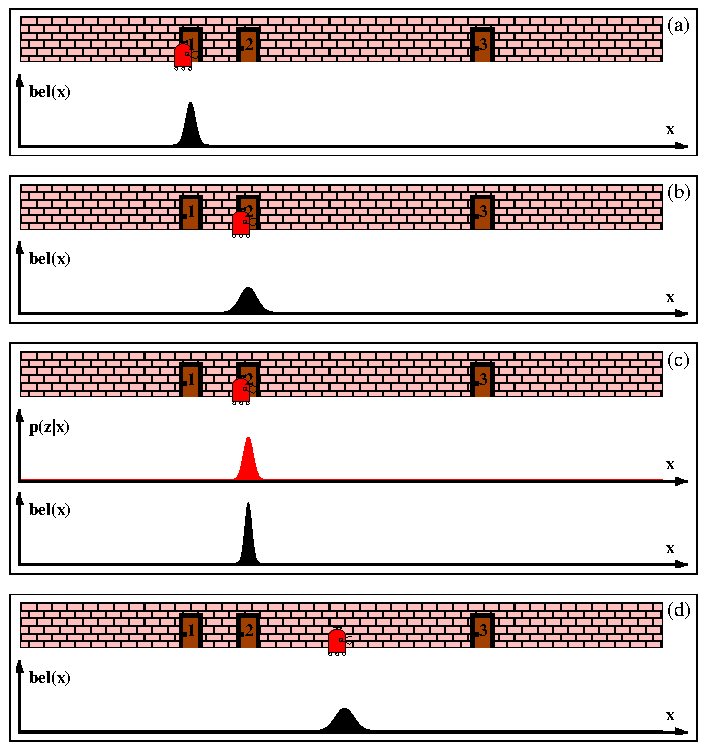
\includegraphics[width = 0.7\textwidth]{Figures/figKalmanFilter.pdf}
  \caption{Kalman Filter demonstration in a one-dimensional environment. Each figure, \textit{(a), (b), (c), (d)} represents a robot and it's positional belief $bel(x)$ as a Gaussian distribution. \textbf{(a):} The robots initial belief. \textbf{(b):} The robots belief after moving and convolving odometry with initial belief. \textbf{(C):} The robot observed the second pillar and gained a posterior probability $p(z|x,M)$. Fusing this with the belief from \textbf{(b)} results in a narrower belief $bel(x)$. \textbf{(d)} Robots belief after moving again and convolving the odometry with the previous belief. Figure from \cite{ThrunSebastian2005Pr}}
  \label{fig:kalmanFilter}
\end{figure}

Kalman Filters assume the system to be linear and with white Gaussian noise. However, most robotic applications are nonlinear. The algorithm therefore has to linearise the system before applying the Kalman Filter \cite{SiegwartRoland2011Itam}. This extension to the original Kalman Filter gives it the name EKF. Linearisation is a simplification of what could otherwise be a complex n-th order system. The result is that the EKF may only work within a certain operating range of the system and may not be helpful at all. For more info on Kalman Filters and EKFs, see \cite{SiegwartRoland2011Itam} or \cite{ThrunSebastian2005Pr}.

\subsubsection{Monte Carlo Localisation}
EKFs are computationally efficient and a great tool to improve probabilistic localisation. However, an EKF based localisation would not be able to do \textit{global localisation} (initial position is unknown, \cite{SiegwartRoland2011Itam}, \cite{ThrunSebastian2005Pr}) or solve the \textit{kidnapped robot problem} (robot gets kidnapped and moved to another location \cite{SiegwartRoland2011Itam} \cite{ThrunSebastian2005Pr}). In this case, a particle based localisation method like Monte Carlo Localisation(MCL) has proven to be successful. Figure \ref{fig:monteCarloLocalisation} is used to better explain how MCL works. The figure and description is adapted from \cite{ThrunSebastian2005Pr}. The figure illustrates a robot in a one-dimensional corridor. The belief $bel(x)$ is represented as pose particles with a height corresponding to their importance factor, hence the particle filter definition. In figure \ref{fig:monteCarloLocalisation}\textit{(a)} the global uncertainty is illustrated through a set of pose particles drawn at random and uniformly over the entire pose space. The robot could be anywhere in the corridor. Then, the robot senses the door and gives a posterior probability $p(z|x)$. MCL gives a importance factor to each particle from the initial particle sampling. The resulting belief$b(x)$ along with $p(z|x)$ can be seen in figure \ref{fig:monteCarloLocalisation}\textit{(b)}. In figure \ref{fig:monteCarloLocalisation}\textit{(c)} the robot has re-sampled the particle set and implemented its movement. It can be seen that the particles are now more densely populated around the most likely poses, but with uniform importance factors. The robot then senses another door and gives the posterior probability $p(z|x)$ again. Looking at figure \ref{fig:monteCarloLocalisation}, it is worth noticing that the posterior probability from \textit{(b)} and \textit{(d)} is equal, as the door sensor won't know the difference between each door. MCL again gives importance factors to each particle, as seen in the belief $bel(x)$ in figure \ref{fig:monteCarloLocalisation}\textit{(d)}. This time, most of the total particle mass is centred around the second door, which is also the robots position according to the illustration. In figure \ref{fig:monteCarloLocalisation}\textit{(e)}, the robot has moved and re-sampled the pose particles, which is centred around the most likely pose of the robot.

\begin{figure}[htp]
  \centering
  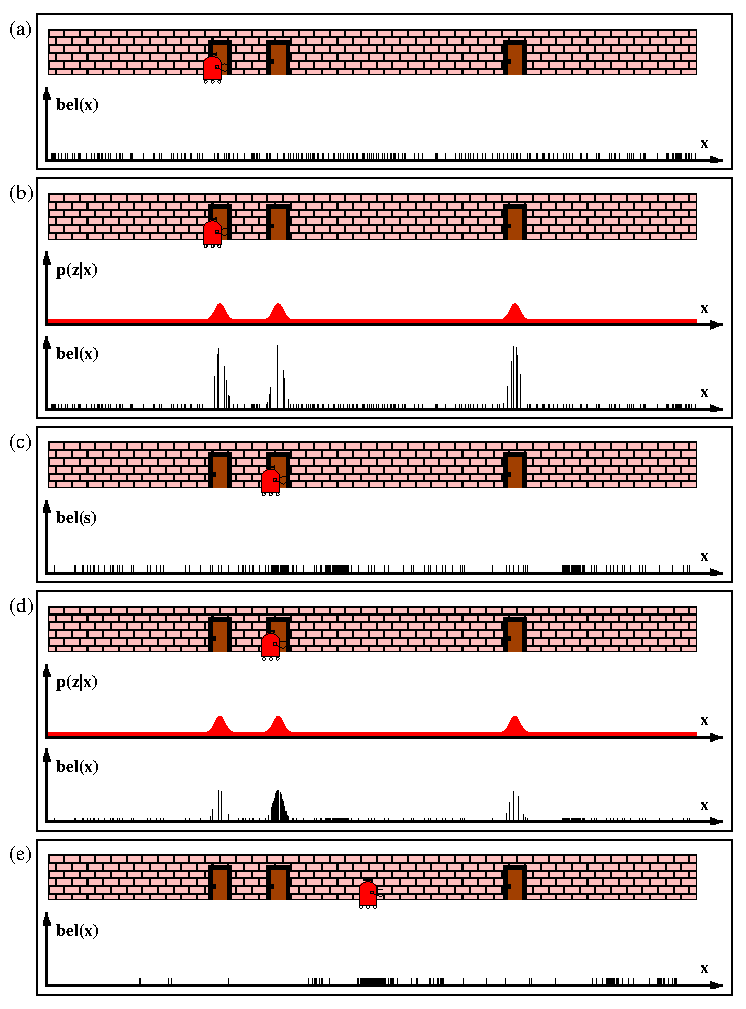
\includegraphics[width = 0.7\textwidth]{Figures/figMCL.pdf}
  \caption{Monte Carlo Localisation a one-dimensional environment. Figure from \cite{ThrunSebastian2005Pr}.}
  \label{fig:monteCarloLocalisation}
\end{figure}

\subsubsection{KLD-Sampling Monte Carlo Localisation}
Plain MCL use particle sample sets of fixed size. At an early stage of localisation, when the robot does not know where it is, the sample set needs to be large to avoid divergence. However, when the location of the robot is fairly confident or known, it is computationally inefficient to have an unnecessarily large particle set. A variant of MCL, called KLD-sampling, adapts the number of particles based on Kullback-Leibler divergence(KLD). Kullback-Leibler divergence is a measure of the difference between two probability distributions. KLD-sampling use KLD to create a measure for the difference between the true posterior belief provided by measurements, and the sample based approximation of this belief. To read more about this localisation method, pleas refer to the source \cite{ThrunSebastian2005Pr}.

\subsection{Simultaneous Localisation and Mapping} \label{sec:T:AN:L:SLAM}
Both EKF-localisation and MCL assumes that it is given a map of the environment. Although there could be a pre-made map that fits the application, this is often not the case. The robot therefore has to do the mapping and localisation at the same time. This problem is called the Simultaneous Localisation and Mapping(SLAM) problem. One of the more popular solutions to the SLAM problem is by the use of pose graphs \cite{Konolige2010}. A pose graph is a sparse graph of nodes with constraints between them. The nodes in the graph are different robot poses and features of the map. The constraints represents the relative relation between the robot poses and also between robot poses and features of the map. It is important to specify that the constraints between the poses are non-rigid. The pose graph can therefore be interpreted as an elastic net of poses. The solution is then to find the state where this net has the minimum amount of energy \cite{SiegwartRoland2011Itam}. Figure \ref{fig:poseGraph} illustrates how a pose graph is built from different robot and map feature poses as a robot moves through an environment. As the map becomes larger, the size of the pose graph also increases, which in turn results in an increased computational effort required for optimisation. A method of pose graph optimisation that has proven efficient, is Sparse Pose Adjustment (SPA)\cite{Konolige2010}. A  map can be constructed as for example an occupancy grid map (described in \cite{ThrunSebastian2005Pr}) when the pose graph is constructed and optimised. \cite{SiegwartRoland2011Itam} and \cite{ThrunSebastian2005Pr} provides more information on SLAM.

\begin{figure}[htp]
  \centering
  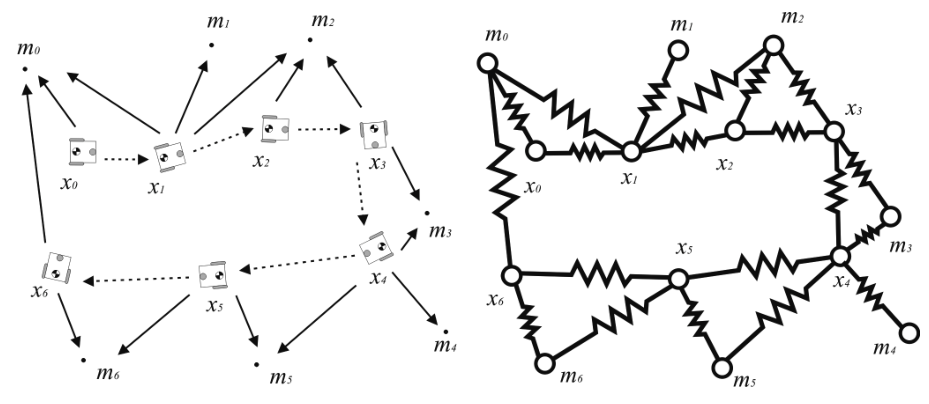
\includegraphics[width = 0.9\textwidth]{Figures/figposeGraph.pdf}
  \caption{Demonstration of pose graph. The illustration demonstrates how robot and map feature poses are presented as nodes with flexible constraints between them to generate a pose graph. Robot poses are denoted as $x_i$ and map feature poses are denoted as $m_n$. Figure from \cite{SiegwartRoland2011Itam}.}
  \label{fig:poseGraph}
\end{figure}


\subsection{Path Planning}\label{T:AN:PathPlaninng}
Path planning involves finding a trajectory that the robot can follow to reach it's goal \cite{SiegwartRoland2011Itam}. Path planning in mobile robotics draws from the extensive research done in this area for robotic manipulators \cite{SiegwartRoland2011Itam}. However, path planning for mobile robots is usually far less complex than that of manipulators due to the reduced degrees of freedom and the fact that manipulators often operate in such high speeds that the dynamics of the system has to be taken into account\cite{SiegwartRoland2011Itam}. A robotic manipulator typically has five or six degrees of freedom, whereas a mobile robot typically operates in a plane with three degrees of freedom. There are numerous different path planning algorithms available, two of the more popular path planning algorithms for use in mobile robotics is Djikstra's Algorithm and A*. When talking about path planning for mobile robotics, a \textit{node} represents a position, often in a grid-based map and an \textit{edge} represent the path from one node to a neighbour node. 

\subsubsection{Djikstra's Algorithm}\label{T:AN:PP:DjikstrasAlgotihm}
Djikstra's algorithm is a planning algorithm published by E. W. Djikstra in 1959\cite{DijkstraE.W1959Anot}. The algorithm presents a way to find the shortest path from a starting point $P_s$ to a goal $P_g$. This is done by giving a cost to the path it finds from $P_s$ to each node in the map, it will keep the paths with the lowest cost and keep searching until it has found the lowest cost path from $P_S$ to all nodes in the map. For each iteration, the algorithm will explore the unexplored node with the lowest calculated cost. The cost is usually based on distance or time taken to traverse the edge. In mobile robotics, the algorithm is often computed from the $P_g$, meaning that it will find the shortest path to any $P_s$ in the map. Thus, the robot is able to plan the best path to the goal based on it's current position without running the planning algorithm again \cite{SiegwartRoland2011Itam}. For example, if the robot is moving towards the goal and needs to take evasive actions because of some moving obstacle in it's trajectory. Time complexity for this algorithm is noted as $O(n\log(n)+m)$ where $n$ is the number of nodes and $m$ is the number of edges\cite{SiegwartRoland2011Itam}. See \cite{DijkstraE.W1959Anot} and \cite{SiegwartRoland2011Itam} for more information about the algorithm. 

\subsubsection{A* Algorithm}\label{T:AN:PP:DjikstrasPlanning}
The A* algorithm is similar to Djikstra's algorithm in that it will give the edges between the nodes a cost. However A* also carries a heuristic which estimates the distance from explored nodes to the goal, $P_g$. For mobile robotics, this heuristic is often calculated as the distance between any cell and the goal cell, $p_g$ in the absence of obstacles (straight distance) \cite{SiegwartRoland2011Itam}. This way, the algorithm will usually explore nodes located in the direction towards the goal before expanding in any other direction. Because of this, the algorithm is often much faster than for example Djikstra's, but it is not guaranteed that the lowest cost path is found. The time complexity of this algorithm is also largely dependent on the weighting of the heuristic and the geometry of the map. See \cite{SiegwartRoland2011Itam} for a more in-depth explanation of the algorithm.

% \subsection{Obstacle Avoidance} \label{T:AN:PP:ObstacleAvoidance}
% Obstacle avoidance refers to the act of avoiding obstacles that are detected by the robot's sensors in order to avoid collision. As an example, if a pedestrian is standing in the robot's trajectory, then the local planner divert the robot so that it moves around the pedestrian instead of running into it. After the evasive action has taken place, the robot should have adjusted it's trajectory so that it can keep following it to reach it's goal. A popular method for obstacle avoidance is the dynamic window approach. This approach takes 

% ------------ØØ - AJ, Do i need to talk about obstacle avoidance/local path planning?  --------------------------------------
% \section{Pick and Place}
% In the context of this thesis, pick and place refers to the complete pipeline of searching for and detecting an object using machine vision, picking it using a robotic manipulator, and placing the object on another location. This section will introduce some different methods for object detection and mention some core concepts on robotic manipulation that is necessary to understand when delving into the work of this thesis.

% \subsection{Machine Vision}
% Machine vision is a 
\section{Object Detection \& Pose Estimation}\label{sec:T:ObjectDetection}
Object detection in the context of this thesis refers to the act of detecting an object in the environment using machine vision. Pose estimation refers to finding the 6-DOF pose of the detected object, that is $x,y,z,\rho, \theta, \phi$ There are a multitude of different methods that could solve this problem. 

\subsection{Machine Learning Based Object Detection \& Pose Estimation}
Machine learning based approaches for object detection and 6-DOF pose estimation could provide a robust
% ----------ØØ - AJ, Do you have a better naming convention for orientation? -------------

\subsubsection{Tag Based Object Detection }\label{sec:T:OD:TagBasedObjectDetection}


% \section{Robot Operating System 2}
% Robot operating system 2 is an open source operating system for robots that is aimed at simplifying the communication between different sensors and actuators in a robotic system, and present the information from these different sensors and actuators in a standardised matter.
% % aj not needed

% \subsection{URDF}
% % aj not needed


%\section{Conclusion}
% we described the building block that forms the basis of our Thesis aimed towards warehouse automation - perception, autonomous navigation, object localization, robotic manipulation. each chapter should have an introduction mentioning what IS covered and end with conclusion mentioning what WAS covered.
\chapter{Method}

% \section{Voxelnet}
% VoxelNet is an End-to-End Learning for Point Cloud Based 3D Object Detection. The work is described in Yin Zhou and Oncel Tuzel's paper: \cite{https://doi.org/10.48550/arxiv.1711.06396}.

% In order to implement this work, the following git repo is adapted: \url{https://github.com/qianguih/voxelnet}. This repo contains a pre-trained model, trained to detect cars from the velodyne lidar data provided by the KITTI dataset.

% \section{ViperX 300 Robot Arm}
% In order to operate the Trossen Robotics ViperX 300 Robotic Arm, Their ROS 2 packages are utilised.
% These can be found here: \url{https://docs.trossenrobotics.com/interbotix_xsarms_docs/}.

This chapter will describe different methodologies used to solve technical problems over the course of this project.

\section{Problem Formulation}

The objective of this project is to set up an autonomous warehouse system where an autonomous UGV should be able to fetch objects in a warehouse. The system will rely on an UGV equipped for autonomous navigation to move around in the environment. The UGV will also be equipped with a robotic manipulator for pick and place operations.

\section{Hardware Setup}
The hardware setup of the system is determined by the tasks that the UGV should preform. The main functionality of the system can be divided into two main subsystems: an autonomously navigating UGV and a robot manipulator for pick-and-place operations. The "Husky A200" by Clearpath is chosen as a the UGV platform for the whole system. This is a ROS 2 compatible UGV with a rugged design that is suitable for both outdoor and indoor applications. The robotic manipulator of choice, is the "Interbotix VX300" by Trossen Robotics. This is a 12V powered compact manipulator that makes it easy to mount on the Husky UGV that has a 12V power distribution. Hardware overview is shown in figure \ref{fig:hardware_overview}.

\begin{figure}[H]
  \centering
  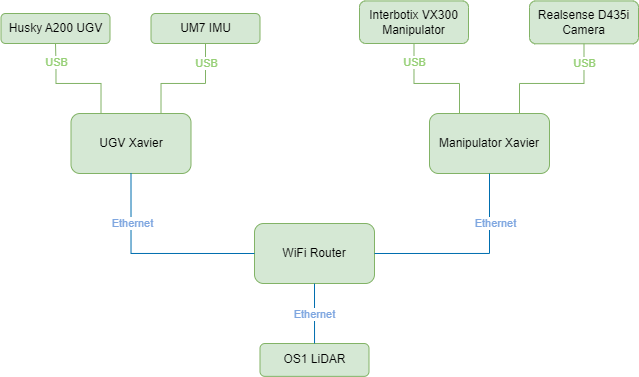
\includegraphics[width = 0.6\textwidth]{Figures/example_figure.drawio.png}
  \caption{Hardware overview of system}
  \label{fig:hardware_overview}
\end{figure}


\section{Software overview}
On a high level, the system is controlled by a ros node called "husky\_master". This node interacts with NAV2 and Moveit 2 to orchestrate an autonomous pick and place operation. The interaction between "husky\_master" and Moveit 2 is done through "husky\_pick\_and\_place" which acts as an interface between Moveit 2 and "husky\_master". A high level overview of this interaction is shown in figure \ref{fig:software_overview}

\begin{figure}[H]
  \centering
  \includegraphics[width = 0.6\textwidth]{Figures/software_overview.drawio.svg}
  \caption{Hardware overview of system}
  \label{fig:hardware_overview}
\end{figure}
\chapter{Results}\label{sec:Results}

In this chapter, the results of this thesis is presented. Section \ref{sec:R:AutonomousNavigaion} presents some results regarding the autonomous navigation system, specifically, SLAM results and navigational results. %Section \ref{sec:R:PickAndPlace} presents results on custom scene publisher pakcage and 
Section \ref{sec:R:TopLevel} presents the results from testing of the complete warehouse automation scenario given in the problem formulation (sec. \ref{sec:I:O:WarehouseScenario}). 

% During the course of this project, an autonomous mobile robot capable of preforming warehouse pick and place tasks has been set up. Necessary mechanical modifications has been done to the UGV platform in order to accommodate extra sensors and a robotic manipulator. Then, sensors and algorithms has been configured to build a demonstration of how this system could be used to preform a warehouse automation task. Testing has first been done separately on both the the autonomous navigation system and the pick and place system. Then, the entire warehouse automation pipeline has been deployed and tested through the Husky Master Node.

 % \section{Hardware}\label{R:Hardware}
 % As hardware aspects and some hardware design has been discussed in section \ref{sec:M:ConceptualDesign} \ref{sec:H:Hardware}, it is natural to include the result of the design process.

% \subsection{General Arrangement} \label{sec:R:GeneralArrangement}
% Looking at figure \ref{fig:huskyComplete}, there is a radar mounting bracket with two Texas Instrument radars at the front of the Husky A200 UGV. This radar array is a part of another Master's Thesis by Didrik Robsrud running in parallel to this project. It is therefore not a part of the general arrangement drawing (figure \ref{fig:general_arrangement}) in section \ref{M:H:GeneralArrangement}. Apart from this radar array, the auxiliary components on the UGV is mounted in accordance to the general arrangement. All components are powered  through the Husky A200's power supply in accordance with the electrical interface drawing (figure \ref{fig:circuit_diagram}) in section \ref{M:H:ElectricalInterface}.



% \subsection{Accessory Mounting Frame}\label{sec:R:H:AccessoryMountingFrame}
% As mentioned in section \ref{sec:M:H:AccessoryMountingFrame}, an accessory mounting frame was made to accommodate auxiliary sensors and equipment. The frame is made out of $20X20[mm]$ aluminium strut profiles \cite{boshRexrothAluminium}, cut to length and put together according to the design in section \ref{sec:M:H:AccessoryMountingFrame}. \ref{sec:M:H:ANH:LidarAndCameraMount}, was fixed to the top of the accessory frame along with the OS1 LiDAR one camera. The complete physical UGV with the it's accessory frame including the LiDAR mount can be seen in figure \ref{fig:huskyComplete}.


% \subsection{Manipulator} \label{sec:R:H:Manipulator}
% The Interbotix VX300 manipulator, described in section \ref{sec:M:H:P&PH:Manipulator}, is mounted to the Husky A200 UGV in accordance with the description. An extra aluminium strut was added at the rear of the UGV to create extra mounting points for the manipulator. It can be seen how the manipulator is mounted on the husky in figure \ref{fig:M:H:CHS:CadHuskyComplete}. 

% \subsection{Manipulator Mounted Camera}\label{R:H:ManipulatorMountedCamera}
% As described in section \ref{sec:M:H:P&PH:ManipulatorMountedCamera}, a manipulator mounted camera has been set up. Section \ref{sec:M:H:P&PH:ManipulatorMountedCamera} also describes how this camera is mounted on the manipulator with a bracket designed for the task. The resulting configuration can be seen in figure \ref{fig:R:H:M:M:MMC:Vx300Complete}.



% \section{Digital Twin} \label{sec:R:DigitalTwin}
% The complete configuration is set up with ROS2 so that a digital twin is possible to visualise in Rviz2. Compatibility with ROS2 allows for example visualisation of the robot on top of a 2D map while autonomously navigating through the environment. Figure \ref{fig:R:H:DT:DigitalTwin} shows the digital twin visualised in Rviz2.


\FloatBarrier
\section{Autonomous Navigation} \label{sec:R:AutonomousNavigaion}
% The autonomous navigation is set up in ROS2 according to the descriptions in the method. In the context of this thesis, the UGV is a part of the autonomously navigating platform. Therefore the resulting configuration of the UGV will be described here. This section will present results regarding the autonomously navigating platform, starting with SLAM and then autonomous navigation results. All testing was preformed at UiA Campus Grimstad.

\FloatBarrier
\subsection{Custom Mobile Robot Bring-up Package}
 The custom mobile ROS 2 package \lstinline{husky_group} described in section \ref{sec:M:AN:CustomMRBringup} is used to bring up the mobile robotic system. As mentioned in section \ref{sec:M:AN:CustomMRBringup} this brings up the entire autonomous navigation system except SLAM and NAV2.
 
 \FloatBarrier
 \subsubsection{Physical Setup}
 The physical mobile robotic system is launched in ROS 2 Foxy Fitzroy. Specifically, the launch file \lstinline{husky.launch.py} is launched on the "UGV Xavier", the computer dedicated to run the mobile robot, as mentioned in section \ref{sec:M:CD:ChoiceOfComponents}. Figure \ref{fig:M:AN:MC:digitalTwin} illustrates how the resulting digital twin of the mobile robot appears in Rviz2.

\begin{figure}[htp!]
  \centering
  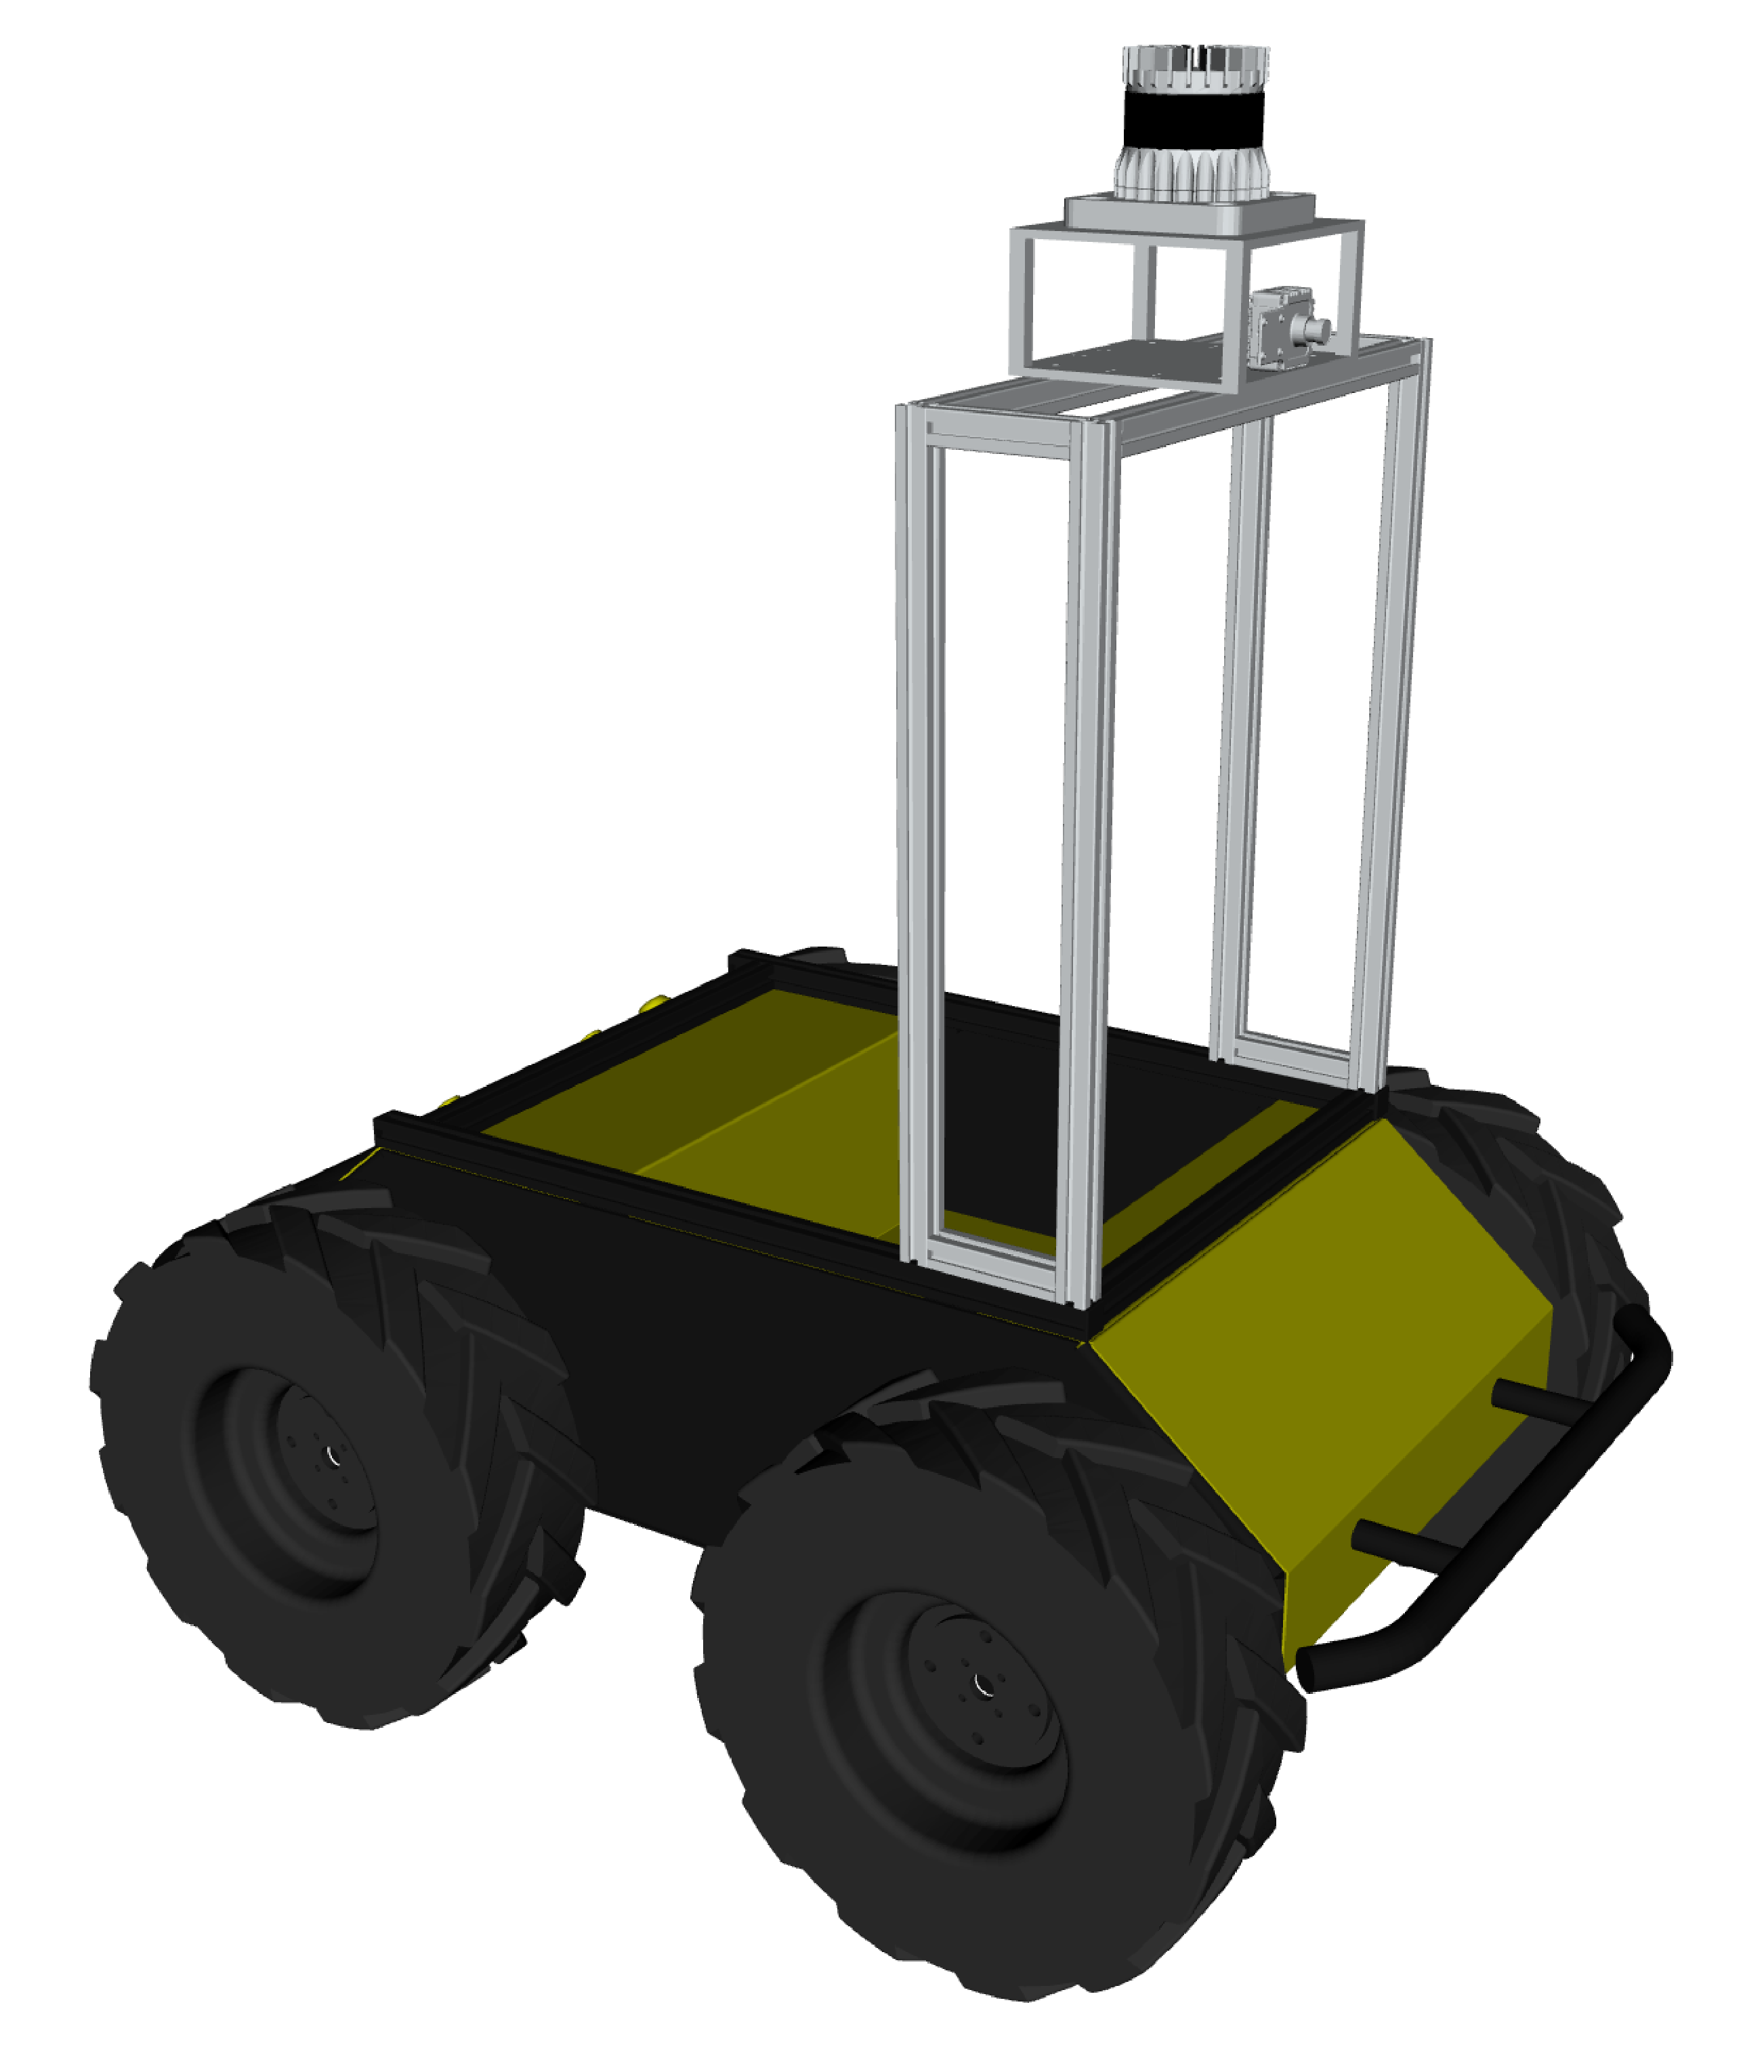
\includegraphics[width = 0.5\textwidth]{Figures/figHuskyRviz.pdf}
  \caption{Rviz2 visualisation of mobile robot running in ROS 2. This acts as a digital twin corresponding to the physical robot.}
  \label{fig:M:AN:MC:digitalTwin}
\end{figure}

\FloatBarrier
\subsubsection{Simulation Setup}
Simulation of the robotic system is run in ROS 2 Galactic Geochelone, by launching \lstinline{sim_husy.launch.py}. This brings up the mobile robot in a Gazebo simulation including a LiDAR simulation. Figure \ref{fig:R:CMR:gazeboSim} illustrates the mobile robot simulated in Gazebo and its digital twin with the corresponding laser scan visualisation in Rviz2.

\begin{figure}[htp!]
  \centering
  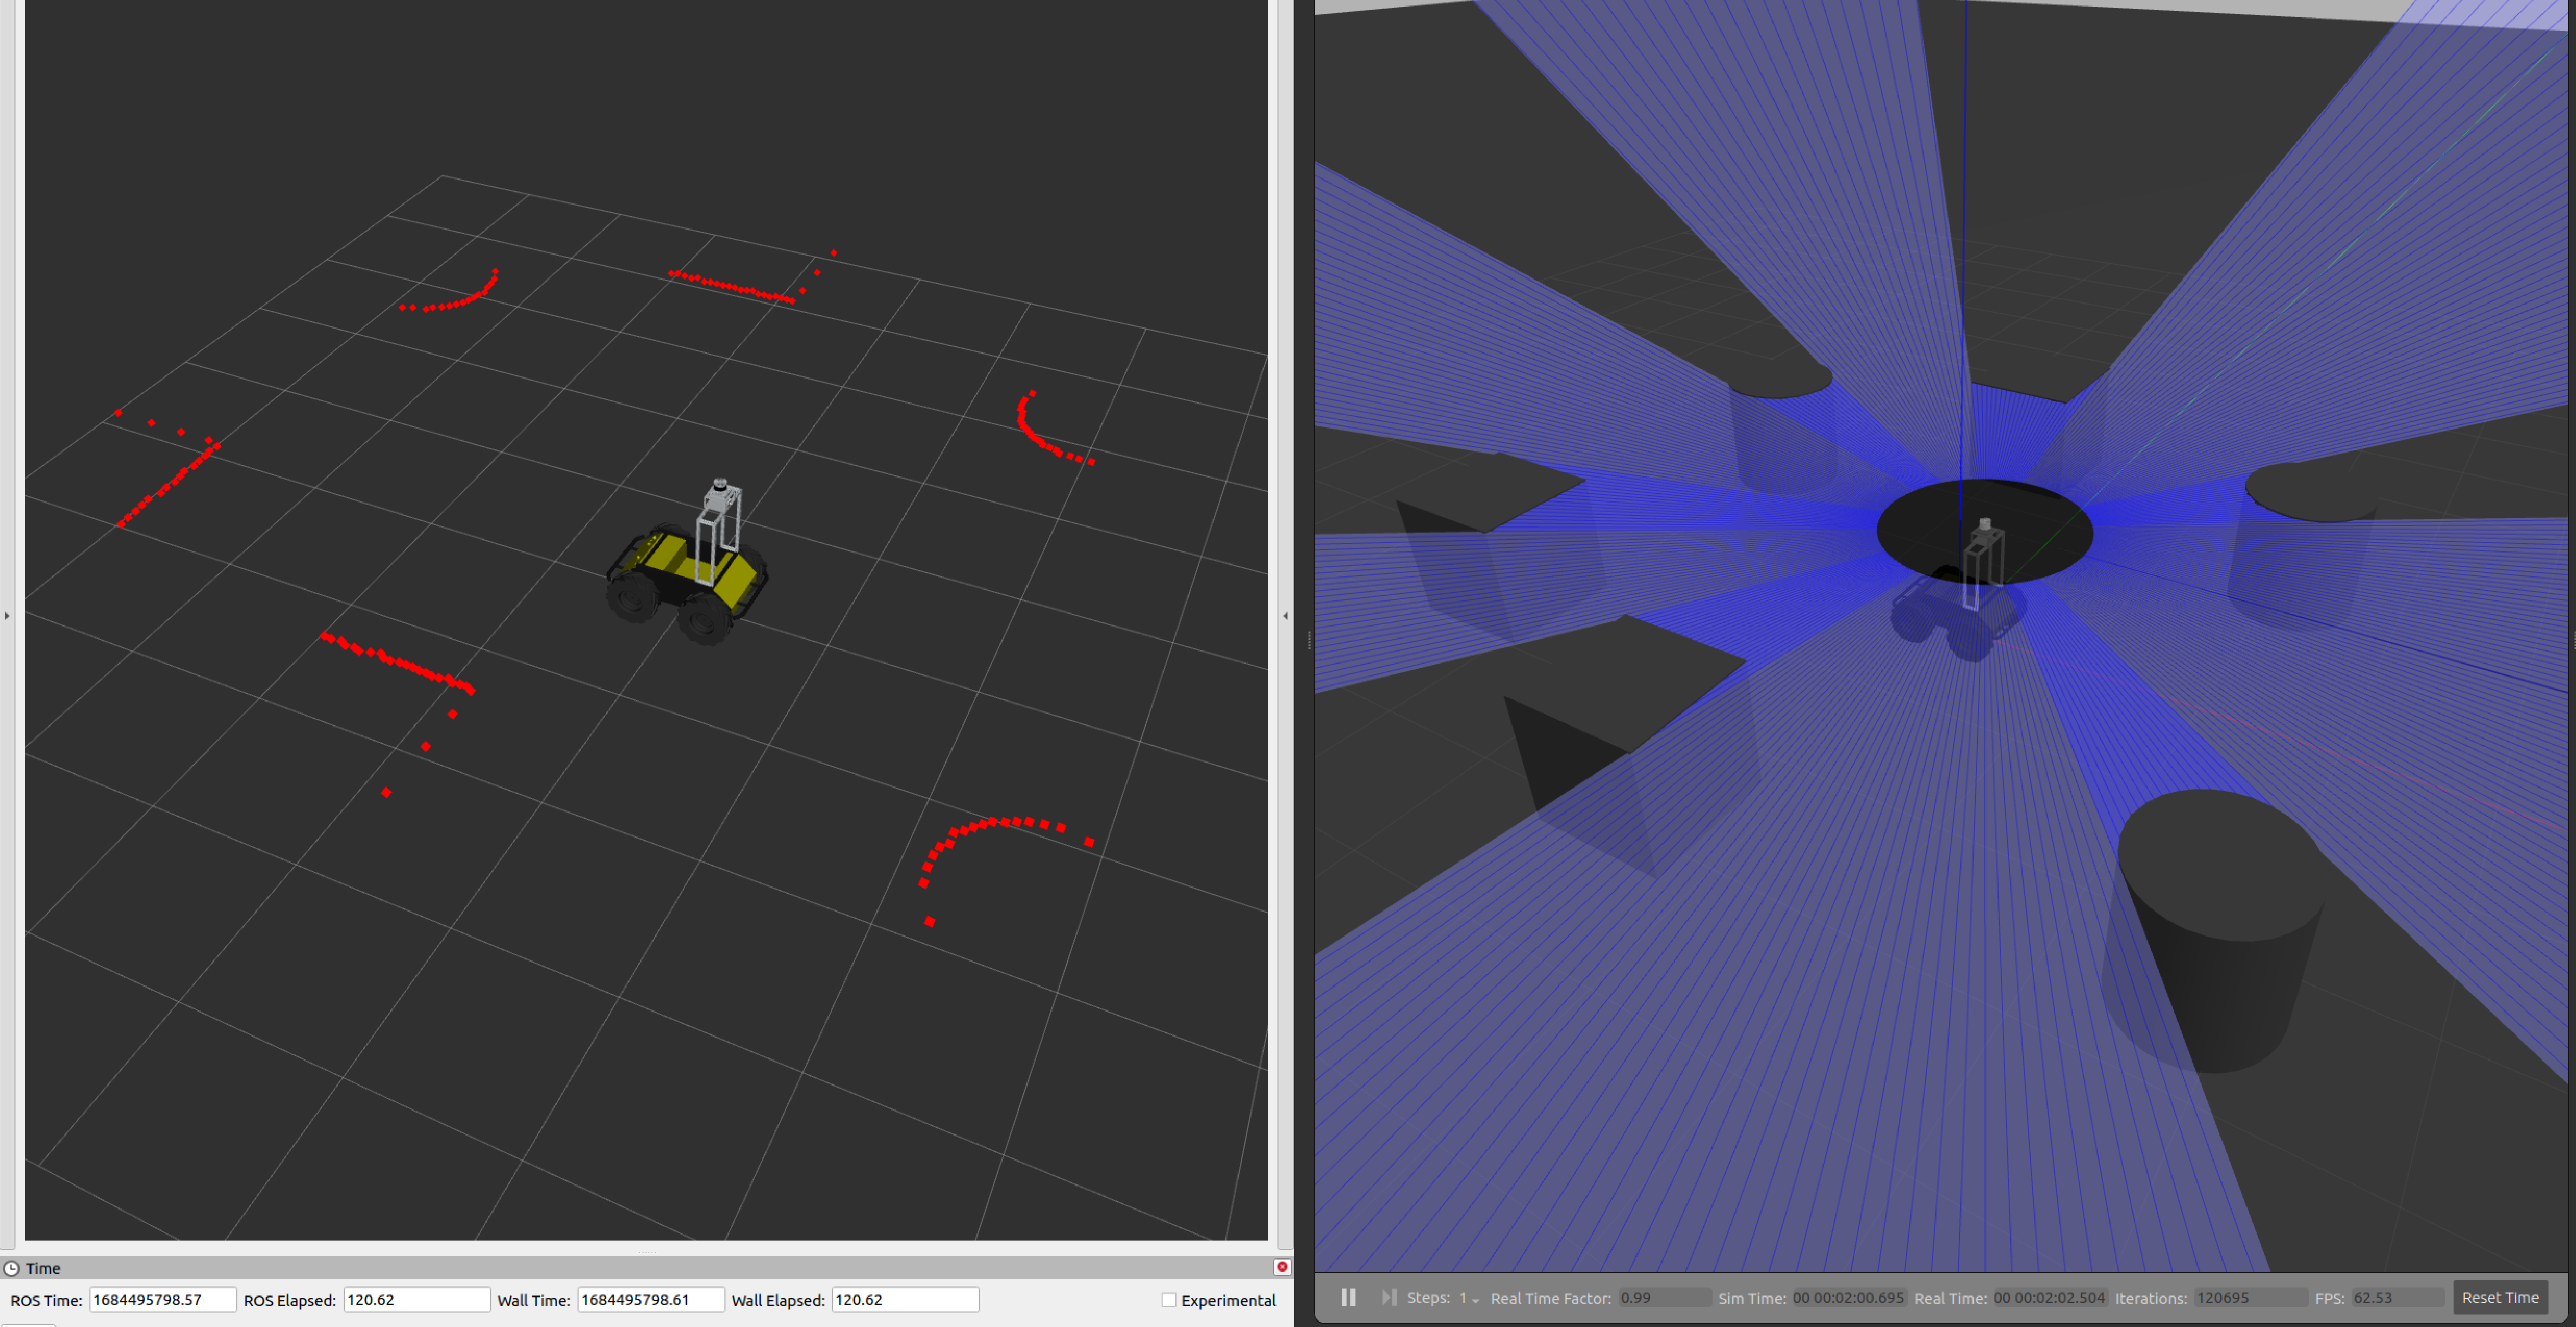
\includegraphics[width = 0.98\textwidth]{Figures/figHuskyGazebo.pdf}
  \caption{Mobile robot simulation running in a Gazebo environment. Corresponding Digital twin and laser scan visualisation can be seen in Rviz2. }
  \label{fig:R:CMR:gazeboSim}
\end{figure}

\FloatBarrier
\subsection{Simultaneous Localisation and Mapping}\label{sec:R:AN:SLAM}

\FloatBarrier
\subsubsection{Physical Experiment}
Physical testing of SLAM performance was done at UiA Campus Grimstad. First mobile robot was launched using \lstinline{husky_launch.py} from the custom ROS 2 package \lstinline{husky_group}. Then SLAM toolbox was launched in online asynchronous mapping with default parameters. NAV 2 is used along with SLAM toolbox to move the mobile robot through the lab. This would generate a map while travelling from the machine lab at campus to the elevators, this is a distance of about \textbf{DISTANCE}, and an area of about \textbf{AREA}. The resulting map can be seen in figure \ref{fig:R:AN:SLAM:figUiaMap}.

\begin{figure}[htp!]
  \centering
  \includesvg[angle=90, width = 0.5\textwidth]{Figures/figUiaMap.svg}
  \caption{Map of Machine Lab and Corridor at UiA Campus Grimstad. The map has been generated through SLAM with an autonomous mobile robot.}
  \label{fig:R:AN:SLAM:figUiaMap}
\end{figure}

\FloatBarrier
\subsubsection{Simulation Experiment}
Performance of SLAM in a simulation environment was tested by launching the mobile robot simulation using \lstinline{sim_husky.launch.py} from the custom ROS 2 package \lstinline{husky_group}. Then a simple environment was created in Gazebo. SLAM Toolbox was then launched in online asynchronous mapping with parameters provided in \lstinline{husky_group} (\lstinline{mapper_params_online_async.yaml}). The mobile robot simulation was then driven around in this Gazebo environment. Figure \ref{fig:R:H:SLAM:figSLAMSim} illustrates the Gazebo test environment along with the corresponding map generated by SLAM.

\begin{figure}[htp!]
  \centering
  \begin{minipage}[b]{0.49\textwidth}
        \centering
        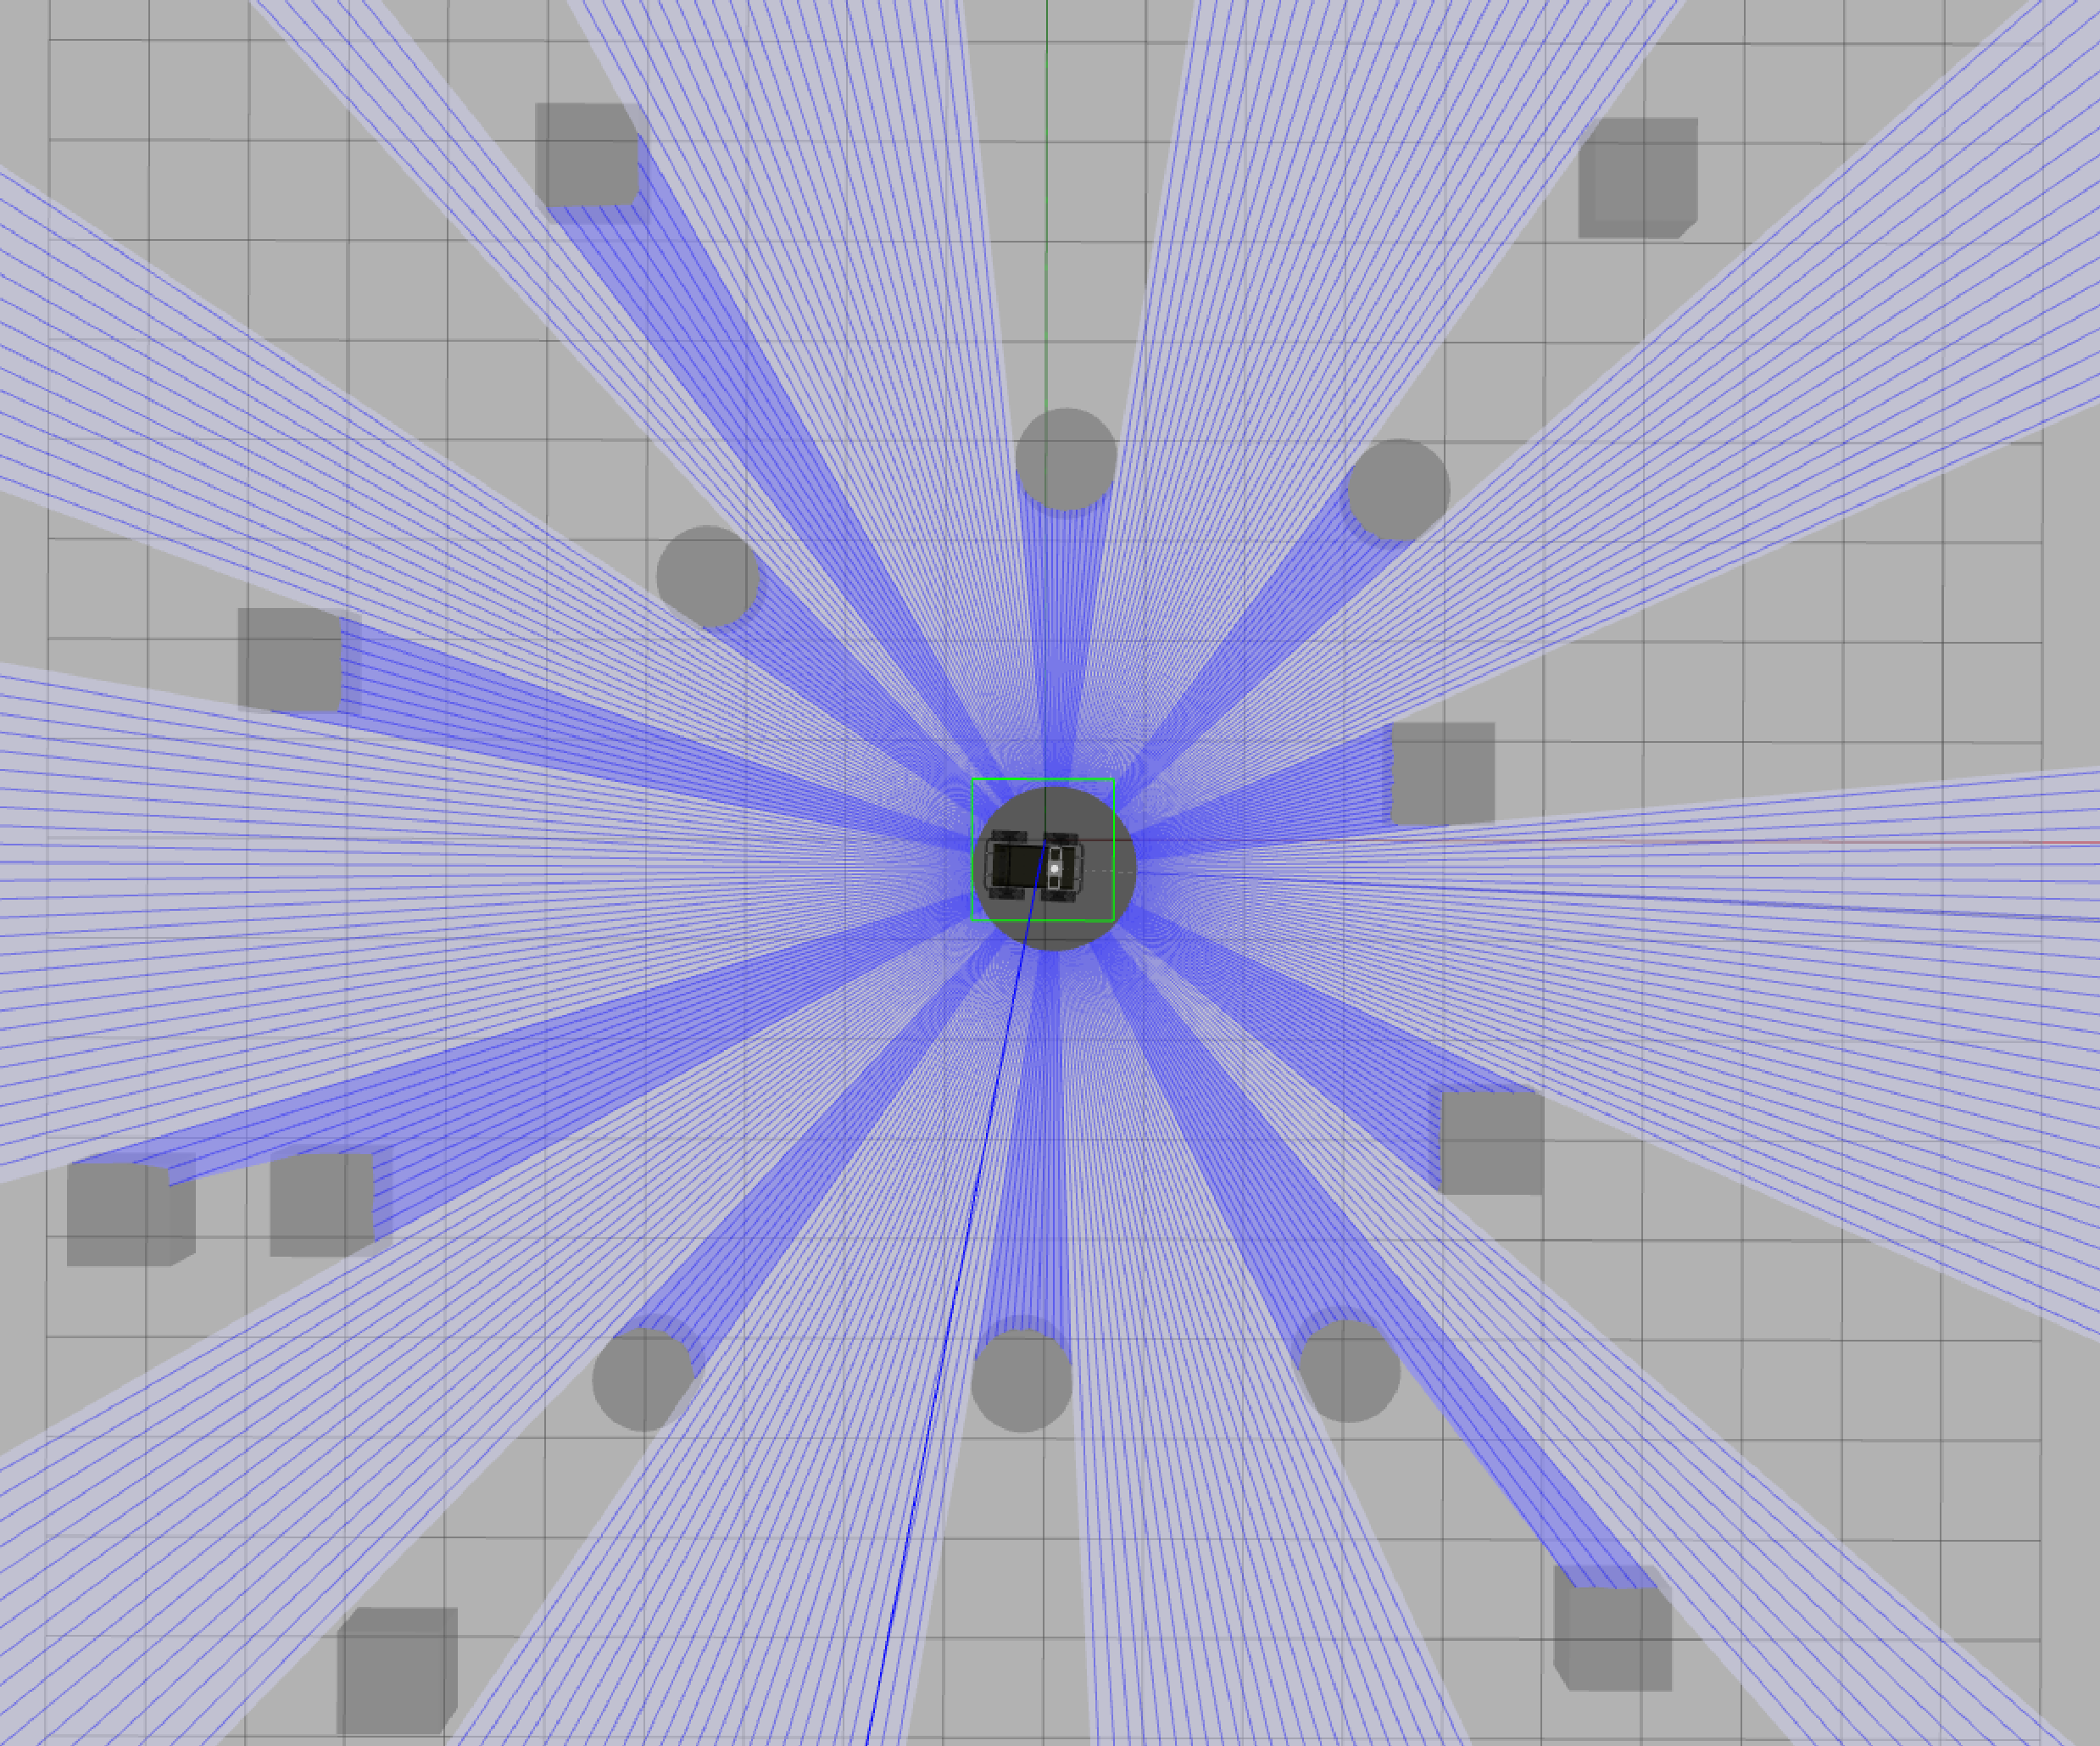
\includegraphics[width = 0.9\textwidth]{Figures/figMapGazeboSim2.pdf}
  \end{minipage}
  \hfill
  \begin{minipage}[b]{0.49\textwidth}
    \centering
    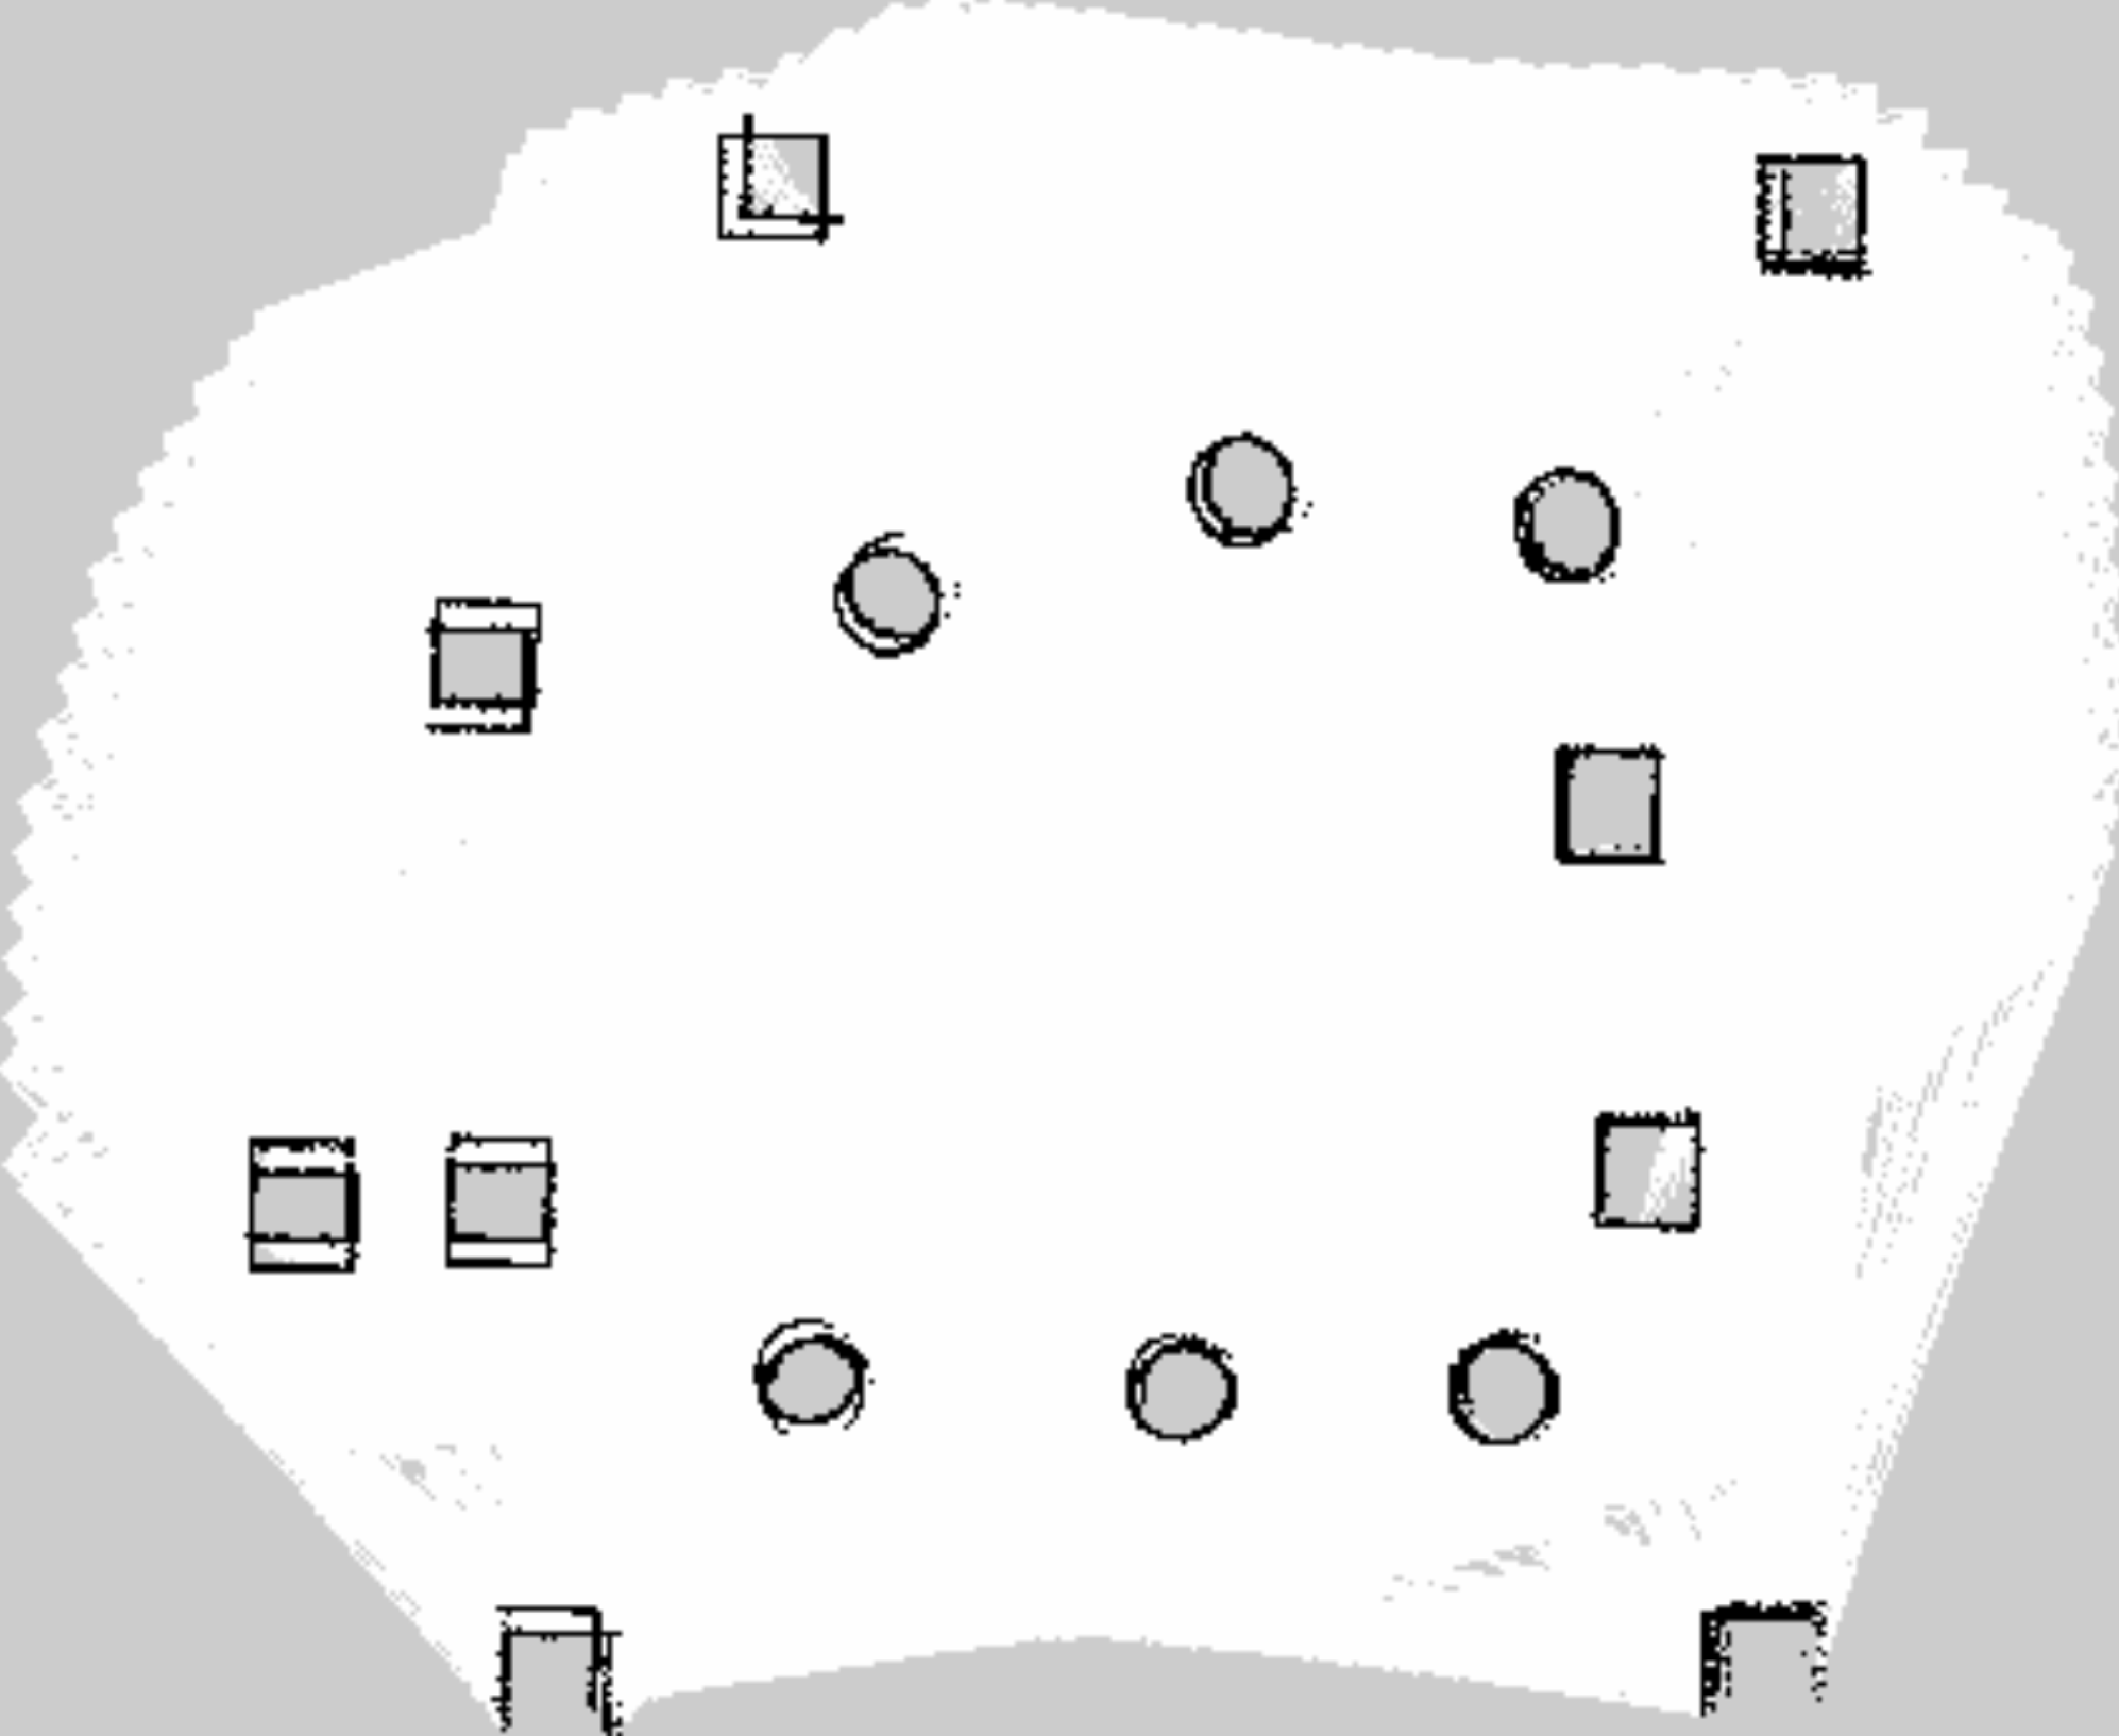
\includegraphics[width = 0.9\textwidth]{Figures/figMapSim.pdf}
  \end{minipage}
  \caption{SLAM testing in Gazebo simulation environment. \textbf{Left:} Gazebo test environment with mobile robot. Laser scan is visualised. \textbf{Right:} SLAM map generated during test in Gazebo test environment.}
  \label{fig:R:H:SLAM:figSLAMSim}
\end{figure}

\FloatBarrier
\subsection{Navigation}\label{sec:R:AN:Navigation}
\FloatBarrier
\subsubsection{Physical Experiment}
Navigation was tested by running the complete setup, together with SLAM, as mentioned in section \ref{sec:R:AN:SLAM}. As the map was generated on-the go, goal poses were manually updated by the operator as the map continued to be updated. Figure \ref{fig:R:H:SLAM:figNavUia} illustrates how the autonomous navigation is visualised on the operators computer using Rviz2.

\begin{figure}[htp!]
  \centering
  \begin{minipage}[b]{0.49\textwidth}
        \centering
        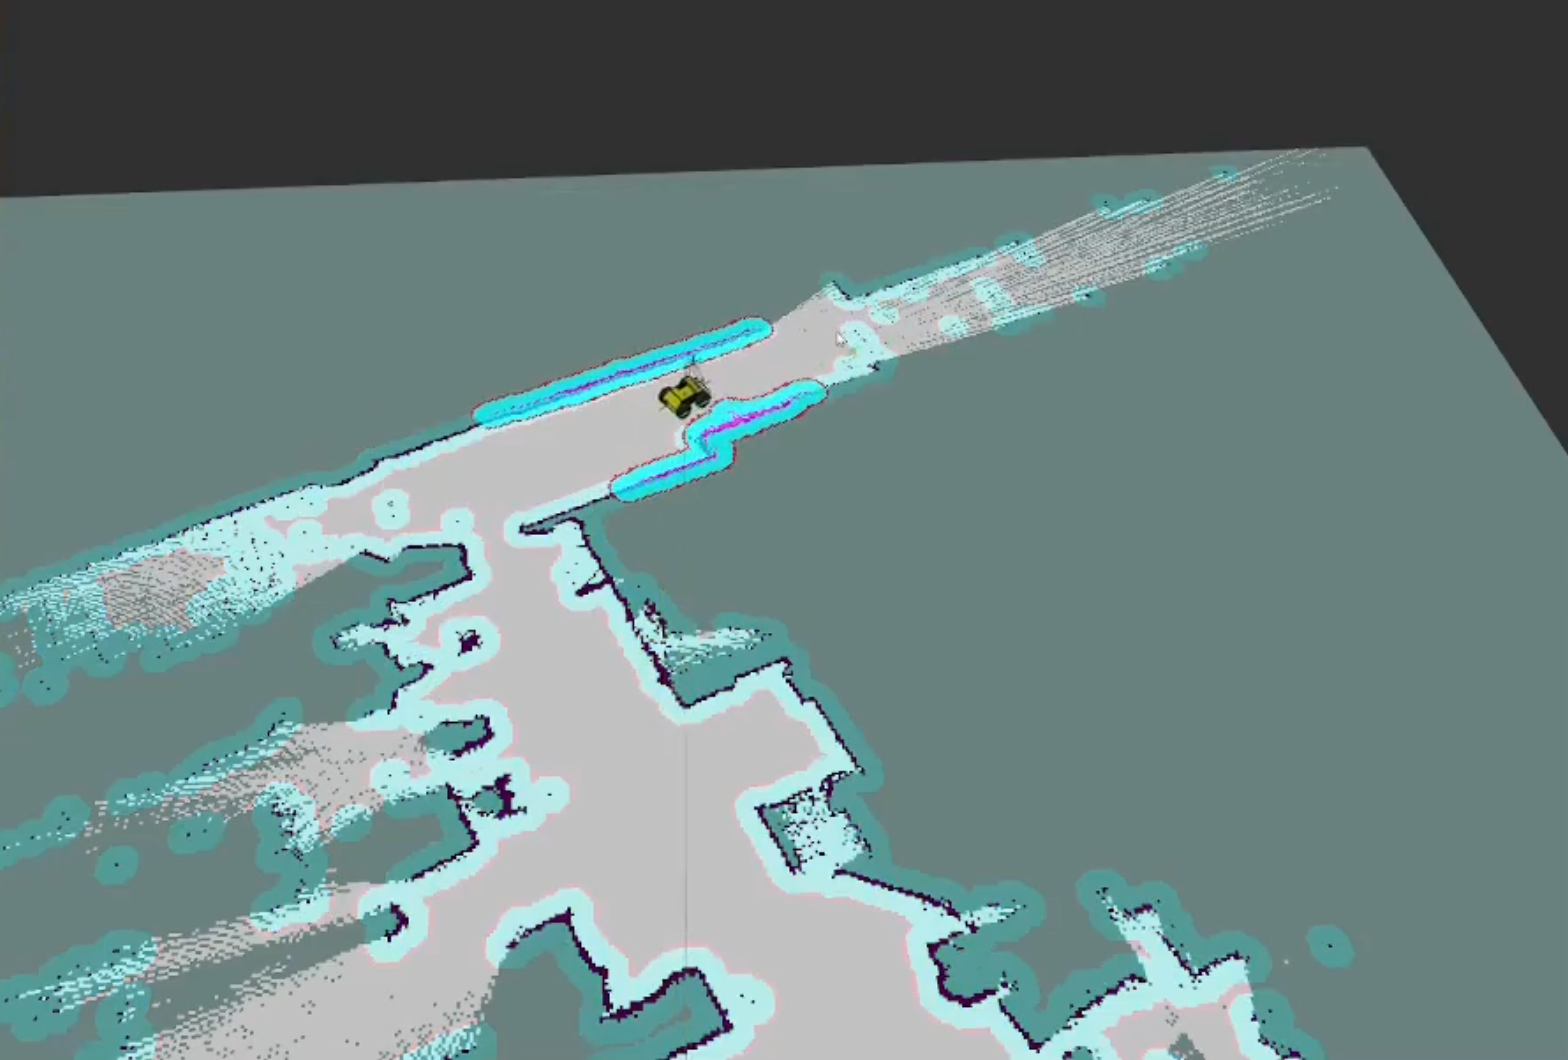
\includegraphics[width = 0.98\textwidth]{Figures/figNavUia2.png}
  \end{minipage}
  \hfill
  \begin{minipage}[b]{0.49\textwidth}
    \centering
    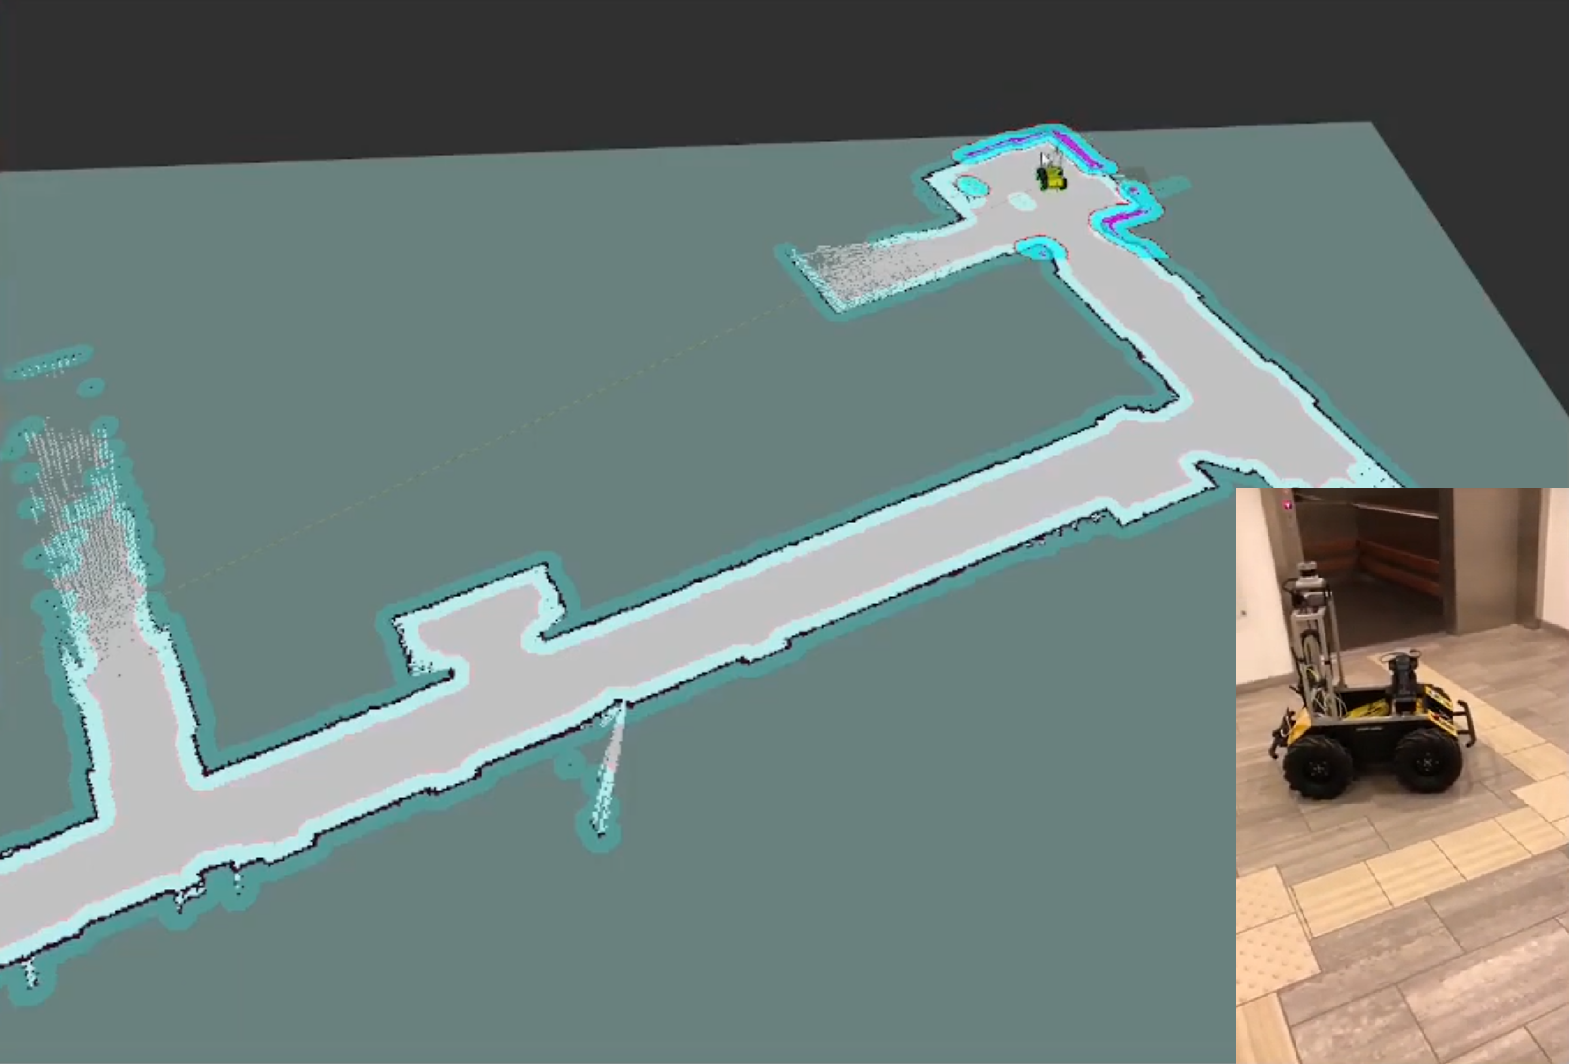
\includegraphics[width = 0.98\textwidth]{Figures/figNavUia4.png}
  \end{minipage}
  \caption{Mobile robot Running NAV2 along with SLAM on ROS2. This is a visualisation of Rviz2 where the mobile robot is illustrated as a 3D model on top of the generated map.}
  \label{fig:R:H:SLAM:figNavUia}
\end{figure}

During navigation testing, collision avoidance was tested by placing a person in front of the robot. Figure \ref{fig:R:AN:N:CA:CollisionAvoidance1} and \ref{fig:R:AN:N:CA:collisionAvoidance2} illustrates this test. In figure \ref{fig:R:AN:N:CA:CollisionAvoidance1} the robot is not close enough to see the pedestrian in its rolling window (pink overlay). A few moments later, a pedestrian has appeared in the rolling window. The resulting trajectory can be seen as the green line in figure \ref{fig:R:AN:N:CA:collisionAvoidance2}.

\begin{figure}[htp!]
  \centering
  \begin{minipage}[b]{0.49\textwidth}
  \centering
    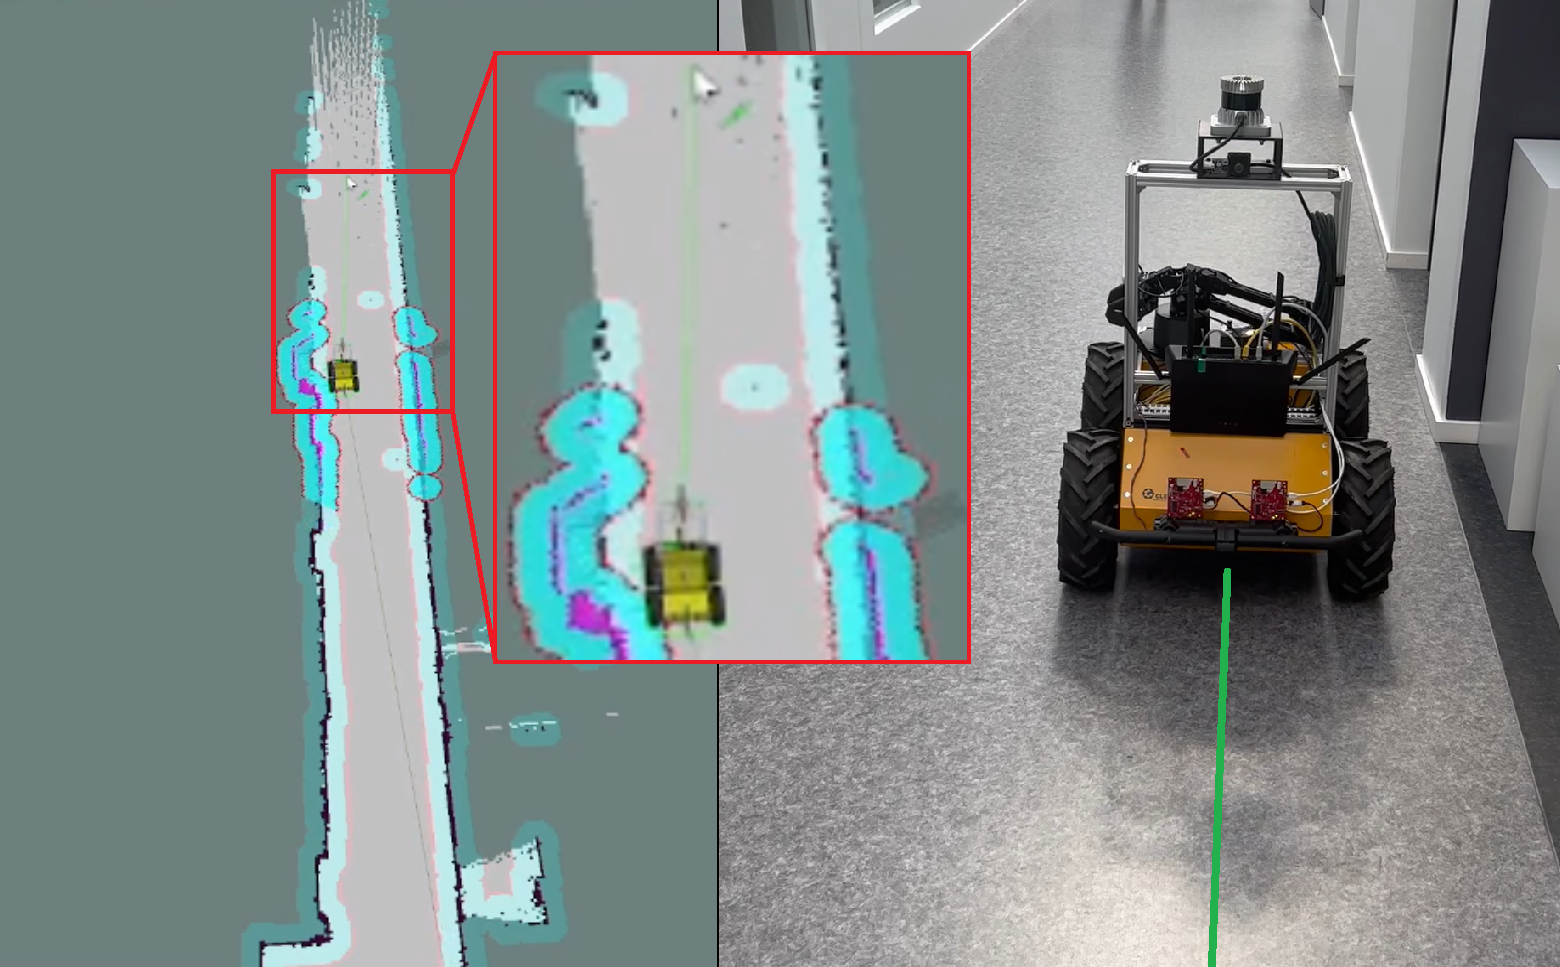
\includegraphics[width = 0.98\textwidth]{Figures/figuiaCollisionAvoidMerged1.png}
    \caption{Robot navigating through a hallway. The robot is not close enough to the camera-man to noctice him in the rolling window. Notice how the trajectory (green line) goes straight forward through the camera-man.}
    \label{fig:R:AN:N:CA:CollisionAvoidance1}
  \end{minipage}
  \hfill
  \begin{minipage}[b]{0.49\textwidth}
    \centering
    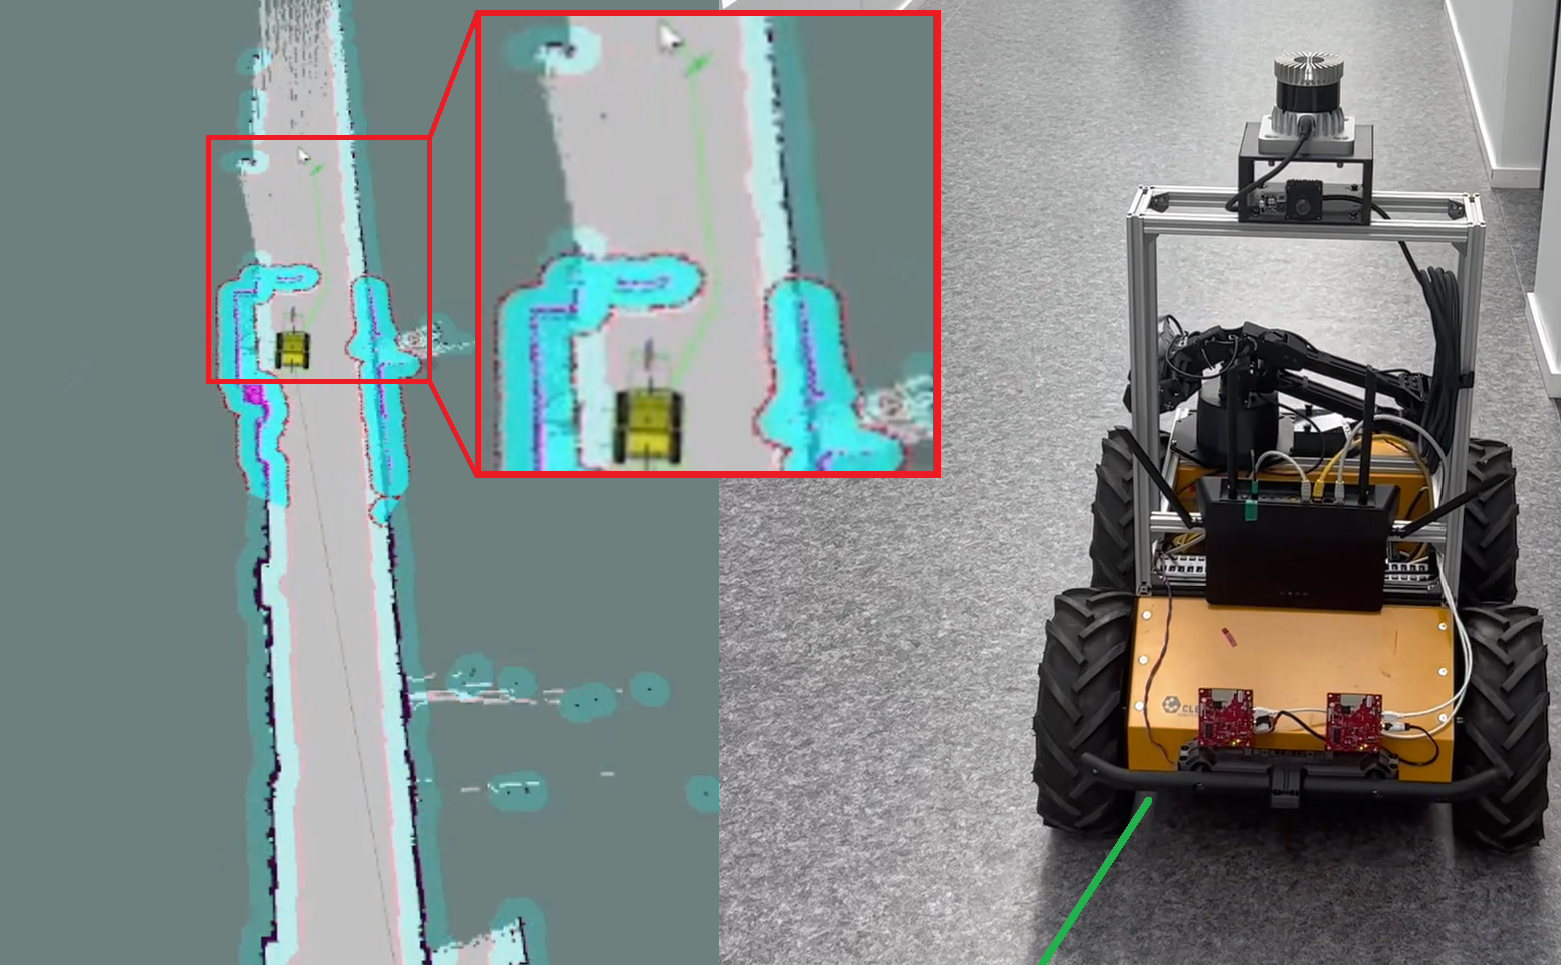
\includegraphics[width = 0.98\textwidth]{Figures/figuiaCollisionAvoidMerged2.png}
    \caption{Robot navigating around obstacle. In this figure, the camera-man can be seen in front of the robot in the rolling window. Notice how the trajectory (green line) goes around the object.}
    \label{fig:R:AN:N:CA:collisionAvoidance2}
  \end{minipage}
\end{figure}

\FloatBarrier
\subsubsection{Simulation Experiment}
Testing of autonomous navigation in a simulation environment was done in a similar way as SLAM simulation testing. First, the mobile robot simulation is launched using \lstinline{sim_husky.launch.py} from the custom ROS 2 package \lstinline{husky_group}. Then, a simple Gazebo environment is created by placing shapes around the mobile robot. SLAM is then launched in online asynchronous mode with parameters provided by \lstinline{husky_group} (\lstinline{mapper_params_online_async.yaml}). The mobile robot is moved around the environment to construct a map. Finally, NAV 2 navigation is launched with parameters provided by \lstinline{husky_group}, and goal poses are set. Figure \ref{fig:R:H:NAV:figNav2Sim} illustrates gazebo test environment along with a map and navigational visualisation in Rviz2.

\begin{figure}[htp!]
  \centering
  \begin{minipage}[b]{0.49\textwidth}
        \centering
        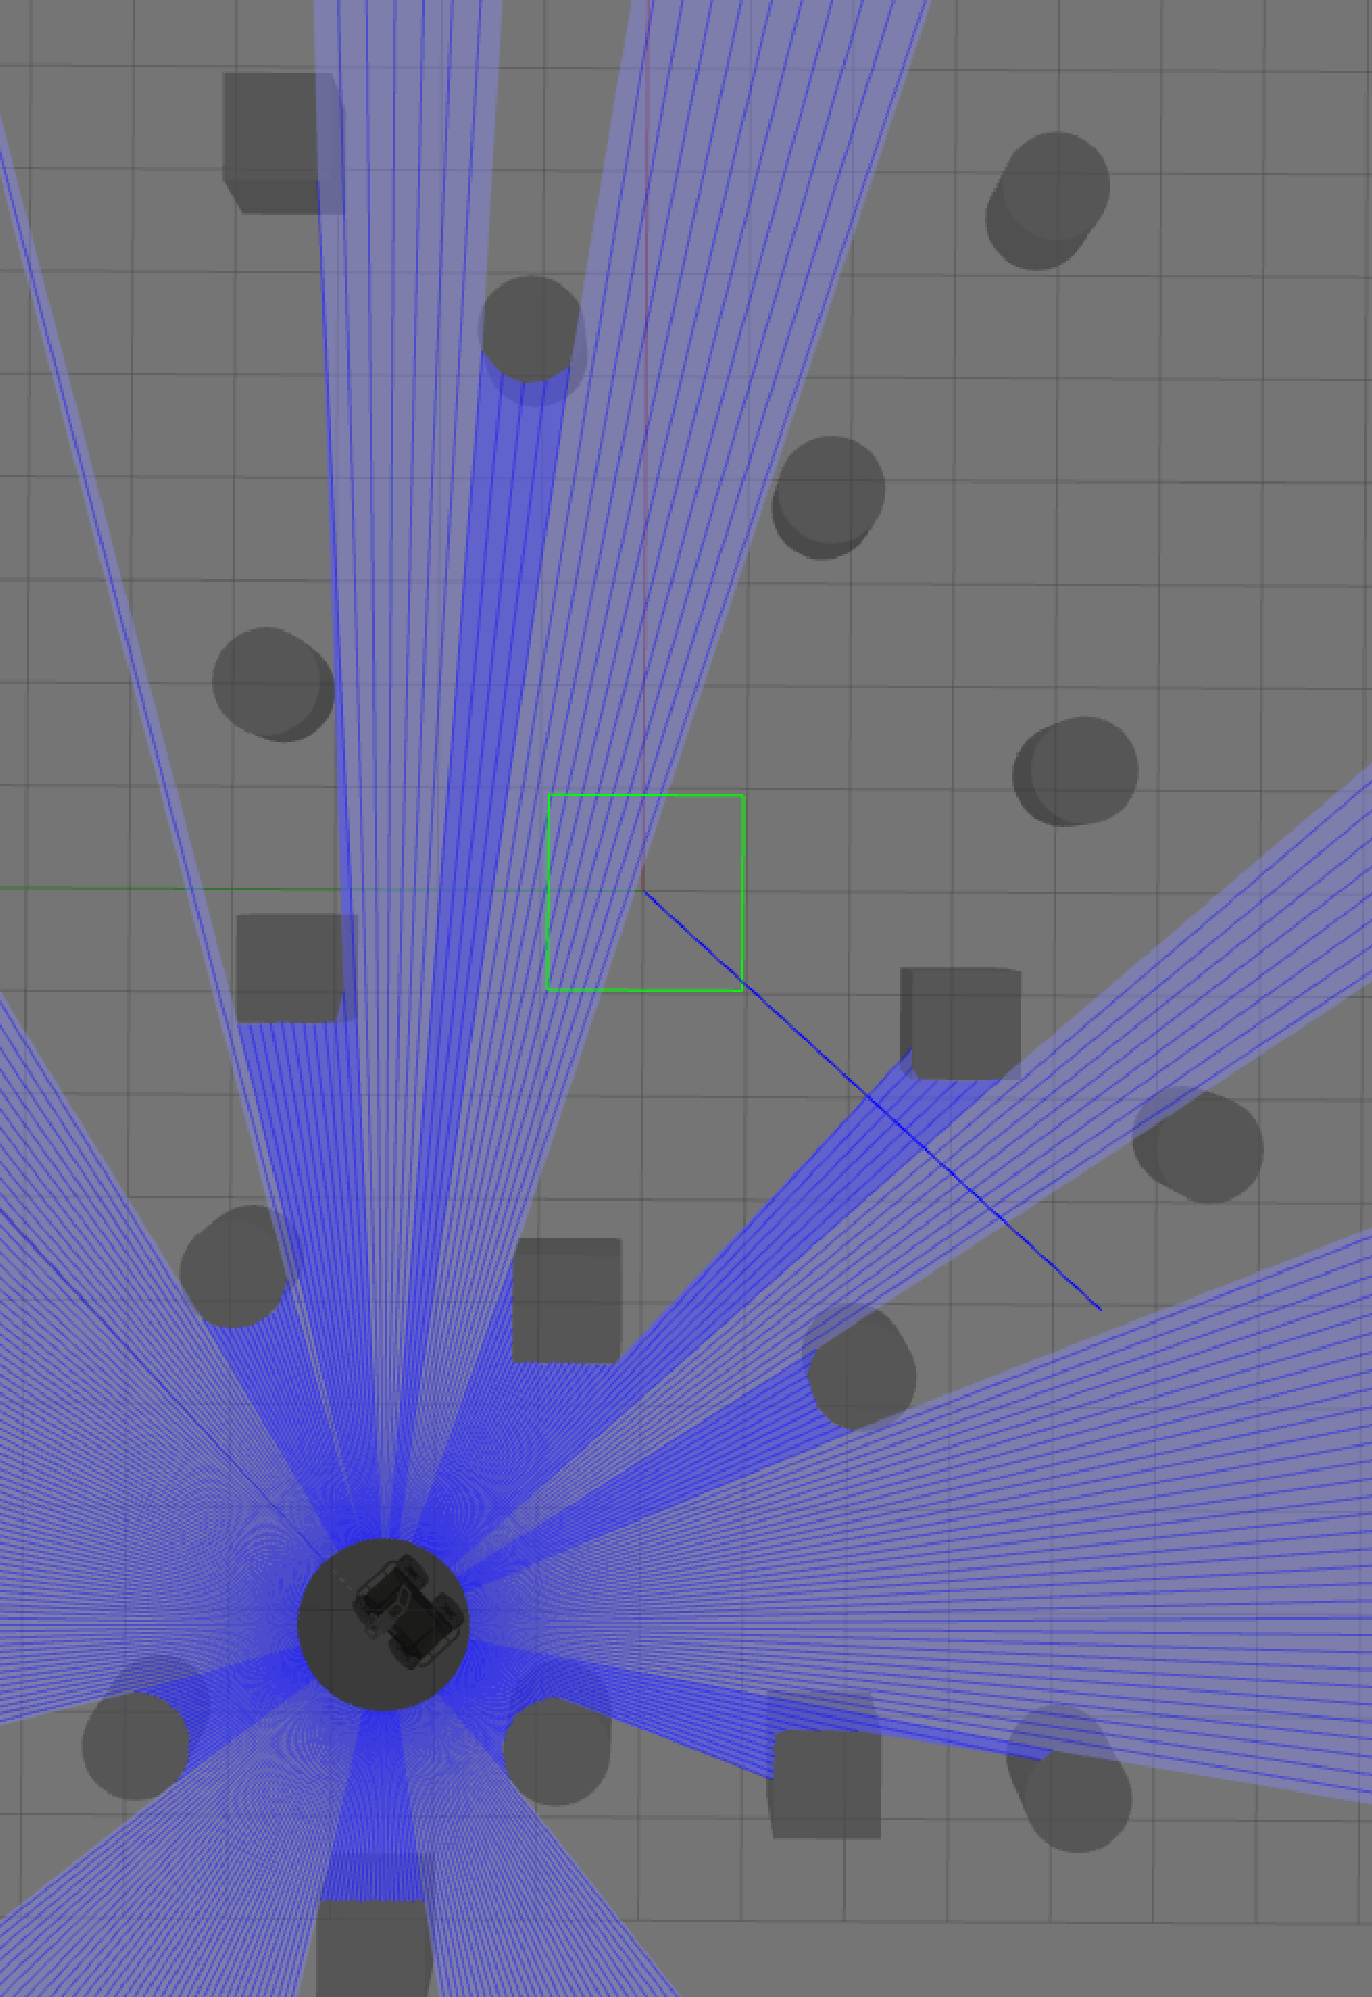
\includegraphics[width = 0.7\textwidth]{Figures/figNav2GazeboSim2.pdf}
  \end{minipage}
  \hfill
  \begin{minipage}[b]{0.49\textwidth}
    \centering
    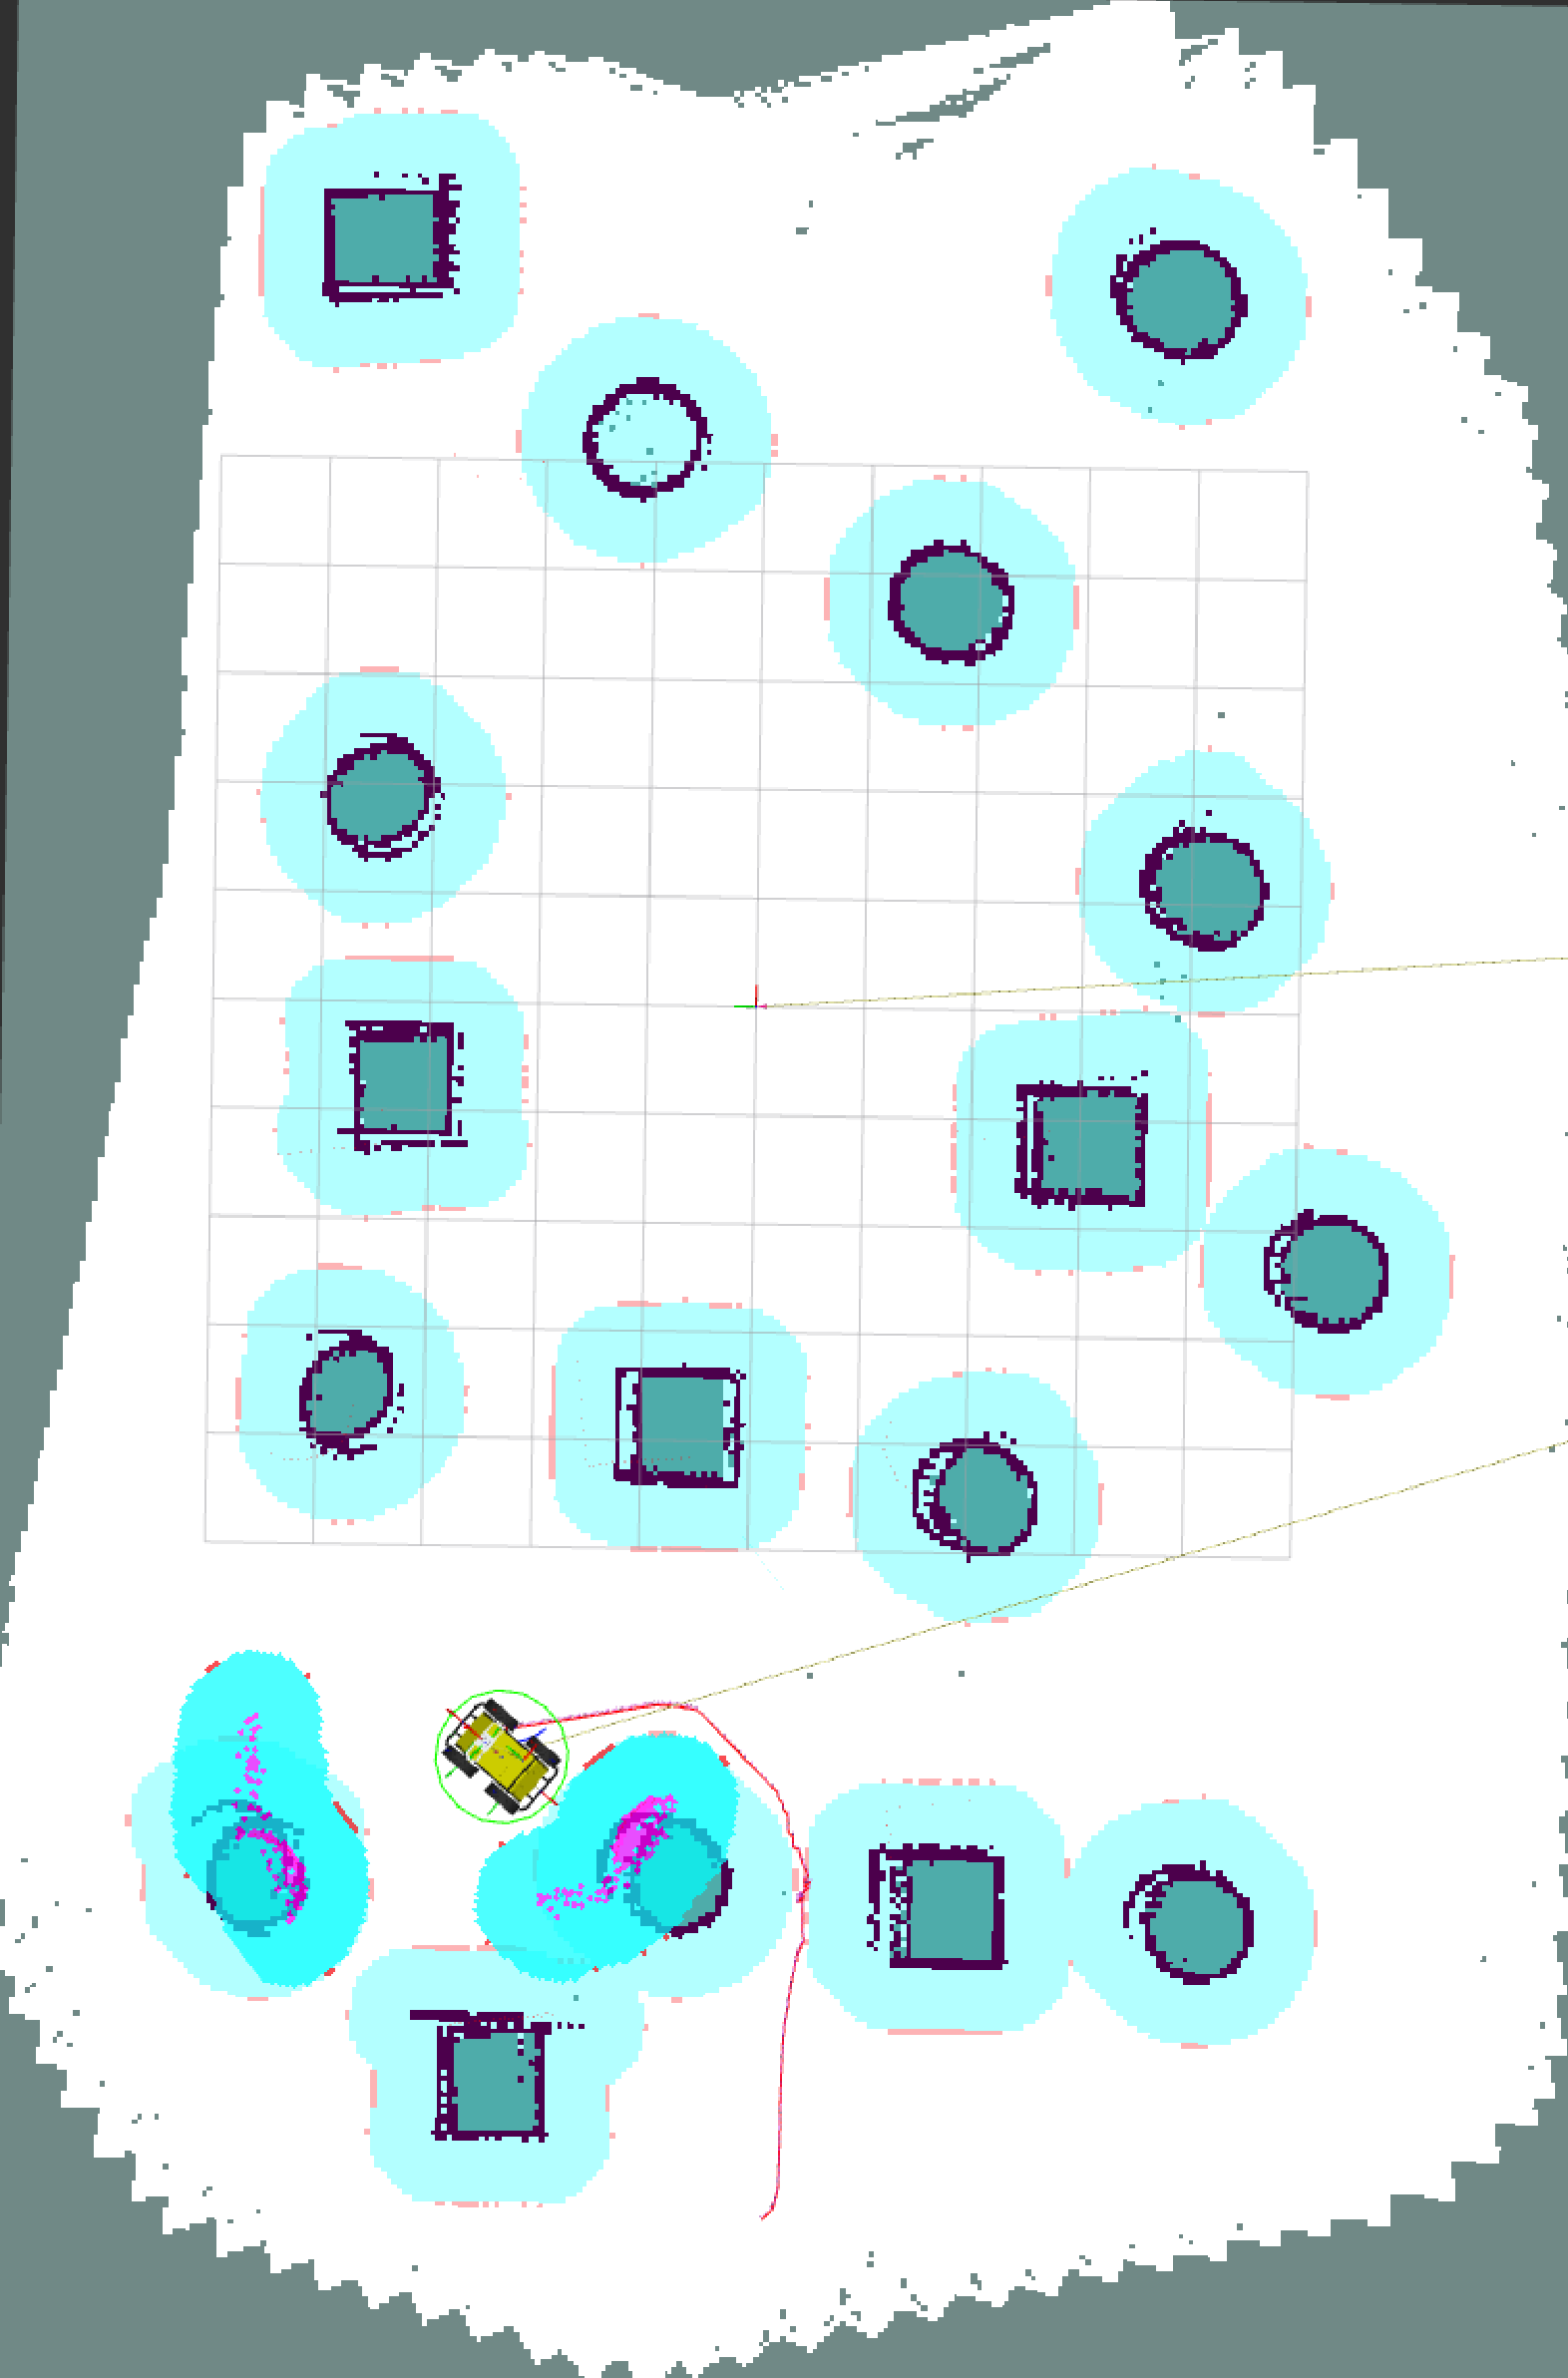
\includegraphics[width = 0.67\textwidth]{Figures/figNav2MapSim2.pdf}
  \end{minipage}
  \caption{NAV 2 testing in simple Gazebo environment. \textbf{Left:} Gazebo simulation test environment with mobile robot. \textbf{Right:} Rviz 2 visualisation of mobile robot moving around in the map constructed from this environment. Red line illustrates planned trajectory.}
  \label{fig:R:H:NAV:figNav2Sim}
\end{figure}

%\section{Pick and Place} \label{sec:R:PickAndPlace}
% Pick and place operations is achieved through a combination of three systems. The first system is the VX300 manipulator itself and it's ROS2 Moveit2 packages described in section \ref{sec:M:MRC:Manipulator}. The second system is the computer vision system described in section \ref{sec:M:MRC:MachineVision}. This includes the vision camera, its drivers and the AprilTag based object detection system. The last system needed is the custom pick and place ROS2 package described in section \ref{sec:M:A:HuskyPickAndPlace}. Results regarding object detection and the custom pick and place ROS2 package will be presented.



% \subsection{Custom ROS2 Packages}
% The custom ROS2 packages has been built and tested around a specific robotic system. It is not likely that it will work for other types of robotic systems out of the box. 

\FloatBarrier
\section{Custom Pick and Place Bring-Up Package}
 The custom mobile ROS 2 package \lstinline{husky_interbotix} described in section \ref{sec:M:PAP:CutsomPAPBringup} is used to bring up the complete pick and place system. As mentioned in section \ref{sec:M:PAP:CutsomPAPBringup} this package can be used with the physical system on the "Manipulator Xavier" as well as a virtual robot for simulation. Figure \ref{fig:R:P&P:CSP:scenePublisher1} illustrates the manipulators visualisation in Rviz 2 with the vision camera mounted to the gripper. Figure \ref{fig:R:P&P:CSP:scenePublisher2} illustrates the collision boxes published to the planning scene by the custom scene geometry publisher (described in method section \ref{sec:M:PAP:SceneGeometryPublisher}) upon launch.

\begin{figure}[htp!]
  \centering
  \begin{minipage}[b]{0.49\textwidth}
        \centering
        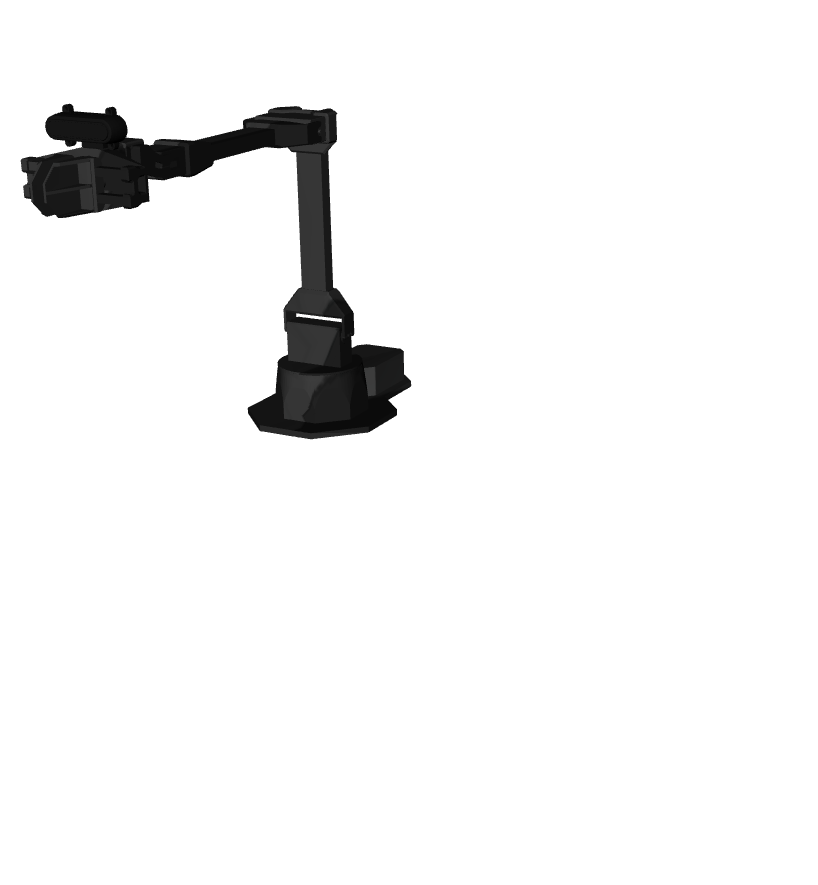
\includegraphics[width = 0.9\textwidth]{Figures/figScenePublisher1.png}
        \caption{Manipulator initiated with Moveit2 and visualised in Rviz2.}
        \label{fig:R:P&P:CSP:scenePublisher1}
  \end{minipage}
  \hfill
  \begin{minipage}[b]{0.49\textwidth}
    \centering
    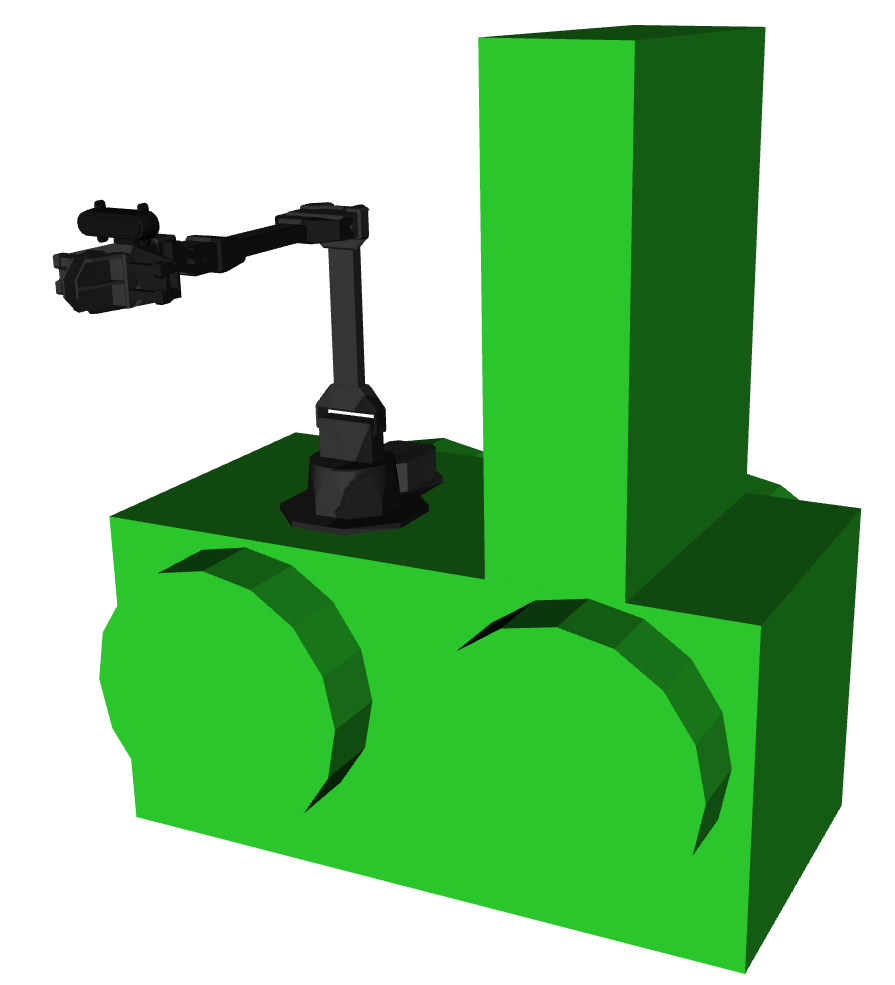
\includegraphics[width = 0.86\textwidth]{Figures/figScenePublisher2.png}
    \caption{Manipulator initiated with Moveit2 and visualised in Rviz2. Collision boxes are published to the planning scene using the custom Scene Publisher ROS2 package.}
    \label{fig:R:P&P:CSP:scenePublisher2}
  \end{minipage}
\end{figure}


% \subsubsection{Husky Pick and Place Package}
% A custom ROS2 package has been made to enable control of the manipulator and get feedback about current operation through the ROS2 network's topic system. The design of this package is described in section \ref{sec:M:A:HuskyPickAndPlace}. Testing has been done to tune the robot's move sequences and to verify the robustness of the ROS2 topic based command and feedback system. 

% \textbf{Do some testing and write a bit about it here}

\FloatBarrier
\section{Top Level} \label{sec:R:TopLevel}
% The full warehouse automation pipeline is set up using the custom ROS2 package "Husky Master Node" described in section \ref{sec:M:A:HuskyMasterNode}. Running this node results in the UGV autonomously navigating to a predefined pick location before running the pick operation. The pick operation includes using computer vision to detect and estimate the pose of the object before picking. After picking, the UGV moves to the place location and the place operation is preformed. Finally, the UGV will return to it's starting position. The complete operation where the robot moves to a pick location, picks an object using MV, moves to a place location, places the object and moves back home was performed twice in a row with success.
The top level system has been tested in three different scenarios:
\begin{itemize}
    \item Physical experiment, with the entire mobile robotic system running in a lab at UiA Campus Grimstad
    \item Simulation experiment, with a simulation of the robotic system running in a simple ROS 2 Gazebo simulation environment. The simulation does not include IMUs, EKF or a computer vision System.
    \item TurtleBot3 Simulation experiment, with a TurtleBot3 gazebo simulation and a virtual Interbotix VX300 robotic arm.
\end{itemize}

Number of navigational goal poses and definition of goal poses have been altered between the tests.

\FloatBarrier
\subsection{Physical Experiment}
Physical testing of the complete warehouse automation pipeline has been performed in the machine lab at UiA Campus Grimstad. Prior to launching the "Husky Master Node" (descried in section \ref{sec:M:TopLevel}), the complete autonomous navigation system including SLAM has been brought in the same way as described in section \ref{sec:R:AN:Navigation}. That is, by first launching the mobile robot using the custom mobile robot bring-up package, then launching SLAM and NAV 2. The pick and place system is also brought up an ready to take commands. This is done using the custom pick and place bring-up package. Figure \ref{fig:R:WA:finalExperiment1} illustrates initiation of the Husky Master node and navigation to the first goal. This is the "pick pose". The complete test was run twice in a row with success.

\begin{figure}[htp!]
  \centering
  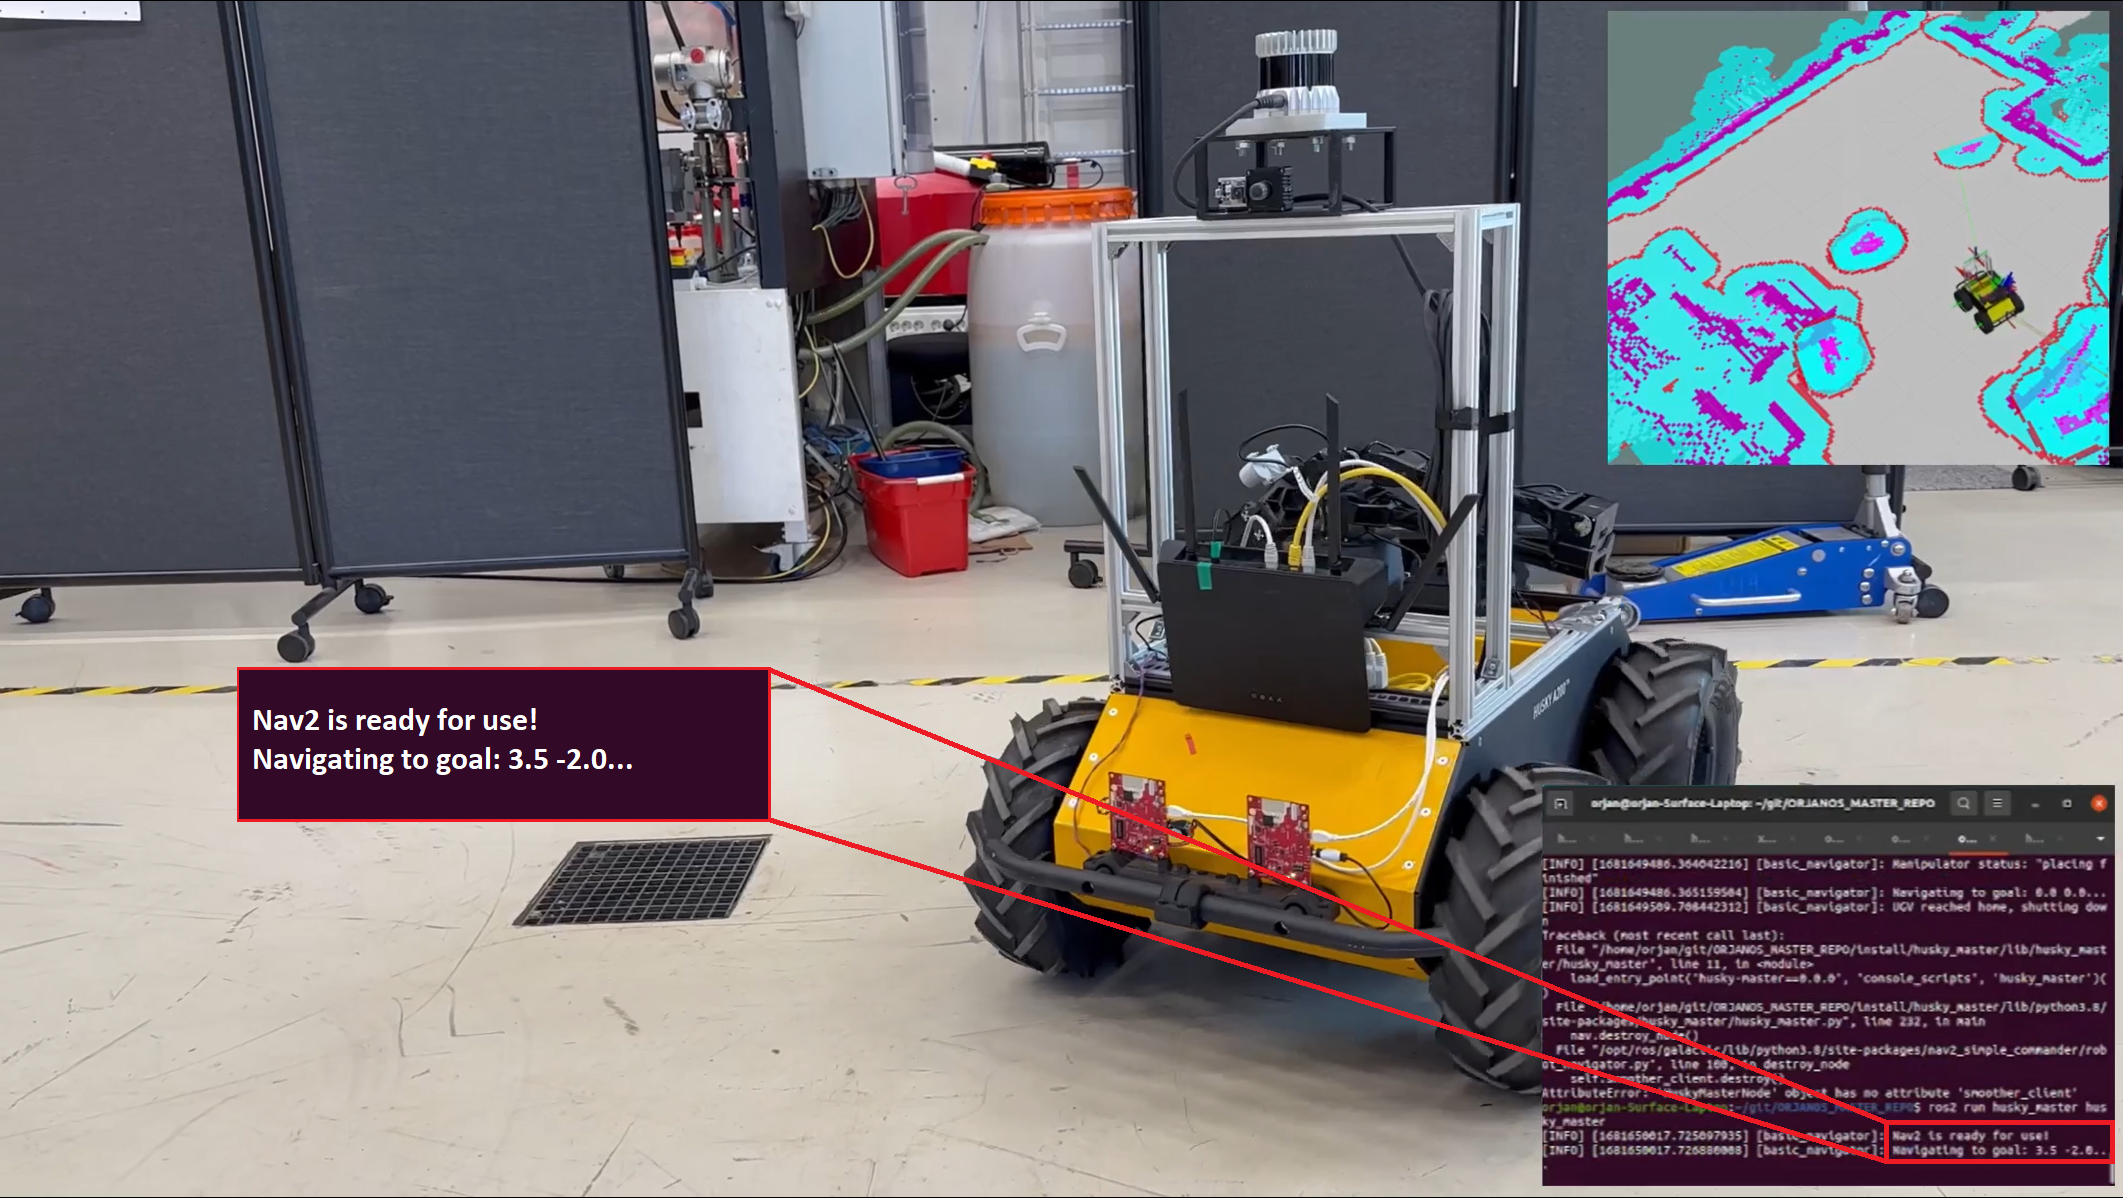
\includegraphics[width = 0.8\textwidth]{Figures/figHuskyFinalExperiment1.png}
  \caption{This figure illustrates initiation of Husky Master Node and navigation towards the first goal during testing. The map in the top right corner corresponds to the actual position of the mobile robot. The terminal window in the lower right corner provides some info about the progress in the warehouse automation pipeline.}
  \label{fig:R:WA:finalExperiment1}
\end{figure}

Figure \ref{fig:R:WA:finalExperiment2} illustrates the picking operation during the warehouse automation task. The mobile robot has reached it's picking pose and is currently performing a picking operation. Interactions between the Husky Master Node and the Pick and Place Node can be seen in the bloated section of the terminal window. The instance figure \ref{fig:R:WA:finalExperiment2} is taken, the manipulator has detected the object, and then placed it's end-effector directly above the object for the computer vision system to get more accurate measurements before picking the object.

\begin{figure}[htp!]
  \centering
  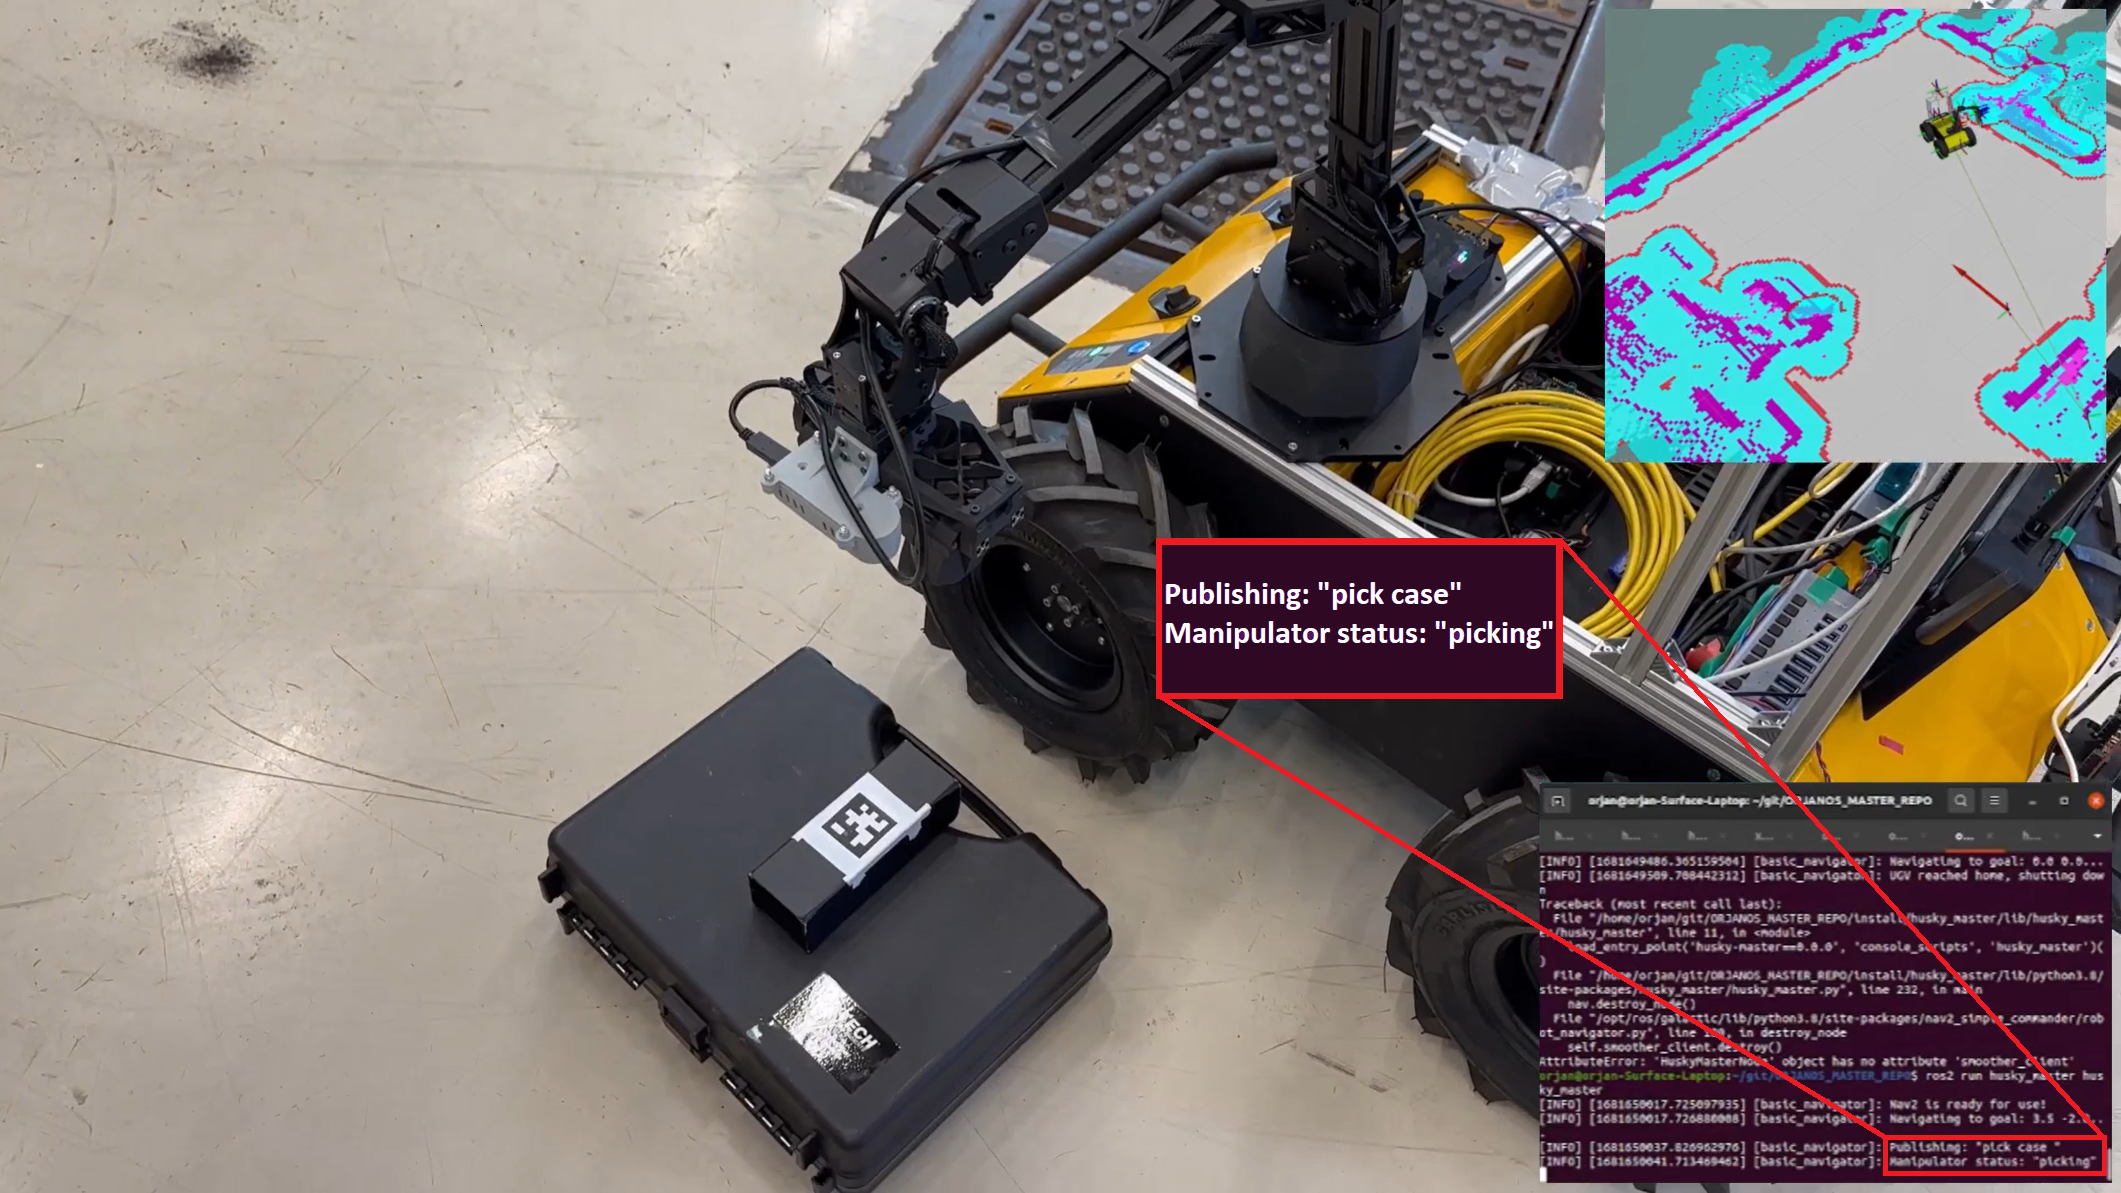
\includegraphics[width = 0.8\textwidth]{Figures/figHuskyFinalExperiment2.png}
  \caption{This figure illustrates picking operation during the warehouse automation task. In this instance, the manipulator has positioned itself directly above the object to give a more accurate measurement before picking. Relevant command and feedback between the Husky Master node and Pick and Place node can be seen in the bloated section from the terminal.}
  \label{fig:R:WA:finalExperiment2}
\end{figure}

% \begin{figure}[htp!]
%   \centering
%   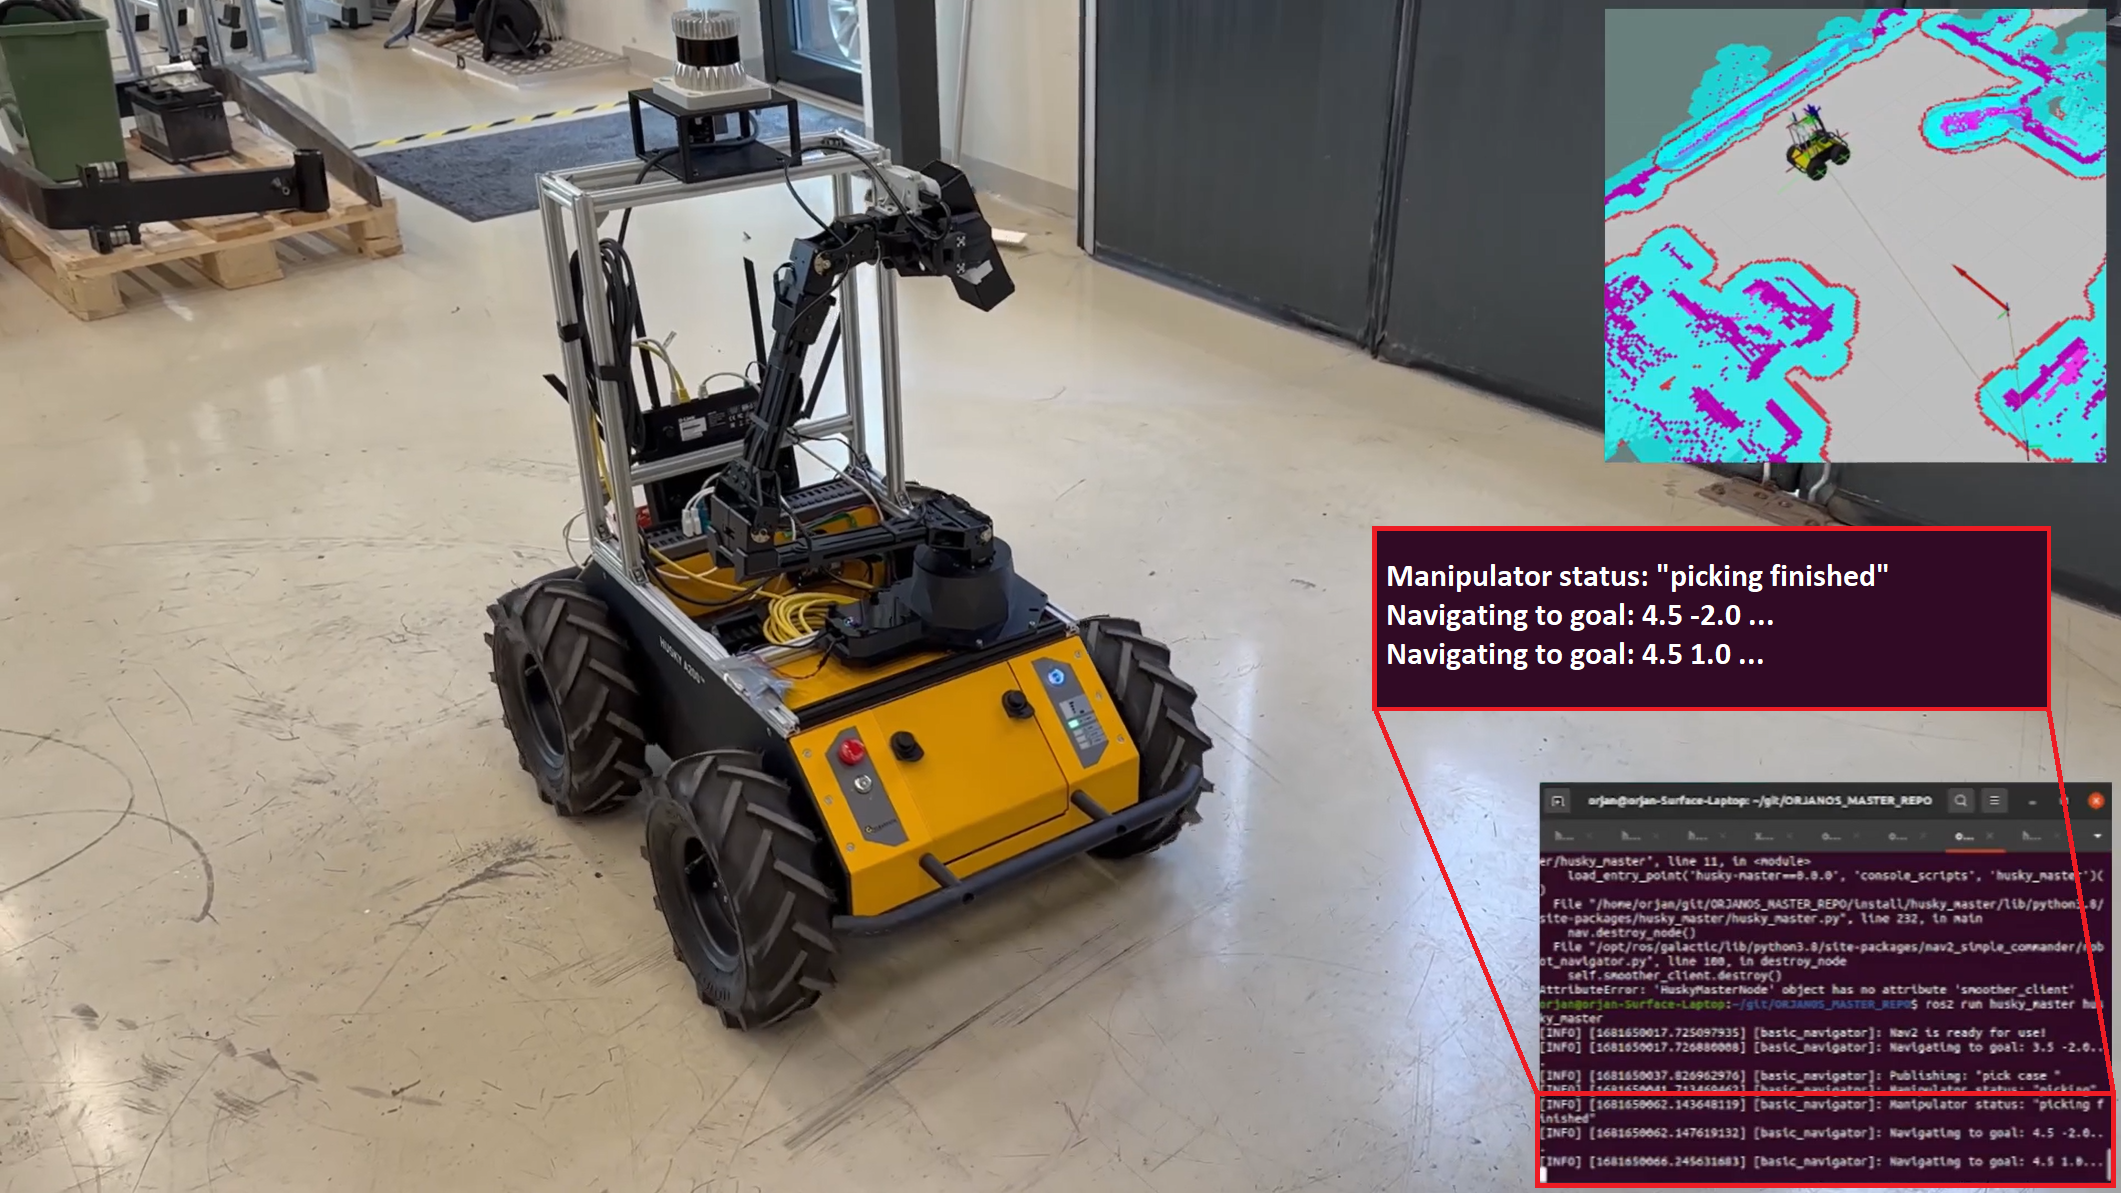
\includegraphics[width = 0.8\textwidth]{Figures/figHuskyFinalExperiment3.png}
%   \caption{This figure illustrates }
%   \label{fig:R:WA:finalExperiment3}
% \end{figure}

The placing operation of the warehouse automation task is shown in figure \ref{fig:R:WA:finalExperiment4}. As with figure \ref{fig:R:WA:finalExperiment2}, interactions between the Husky Master Node and the Pick and Place Node can be seen in the bloated terminal section. The object has been dropped to the floor moments before figure \ref{fig:R:WA:finalExperiment4} is captured.

\begin{figure}[htp!]
  \centering
  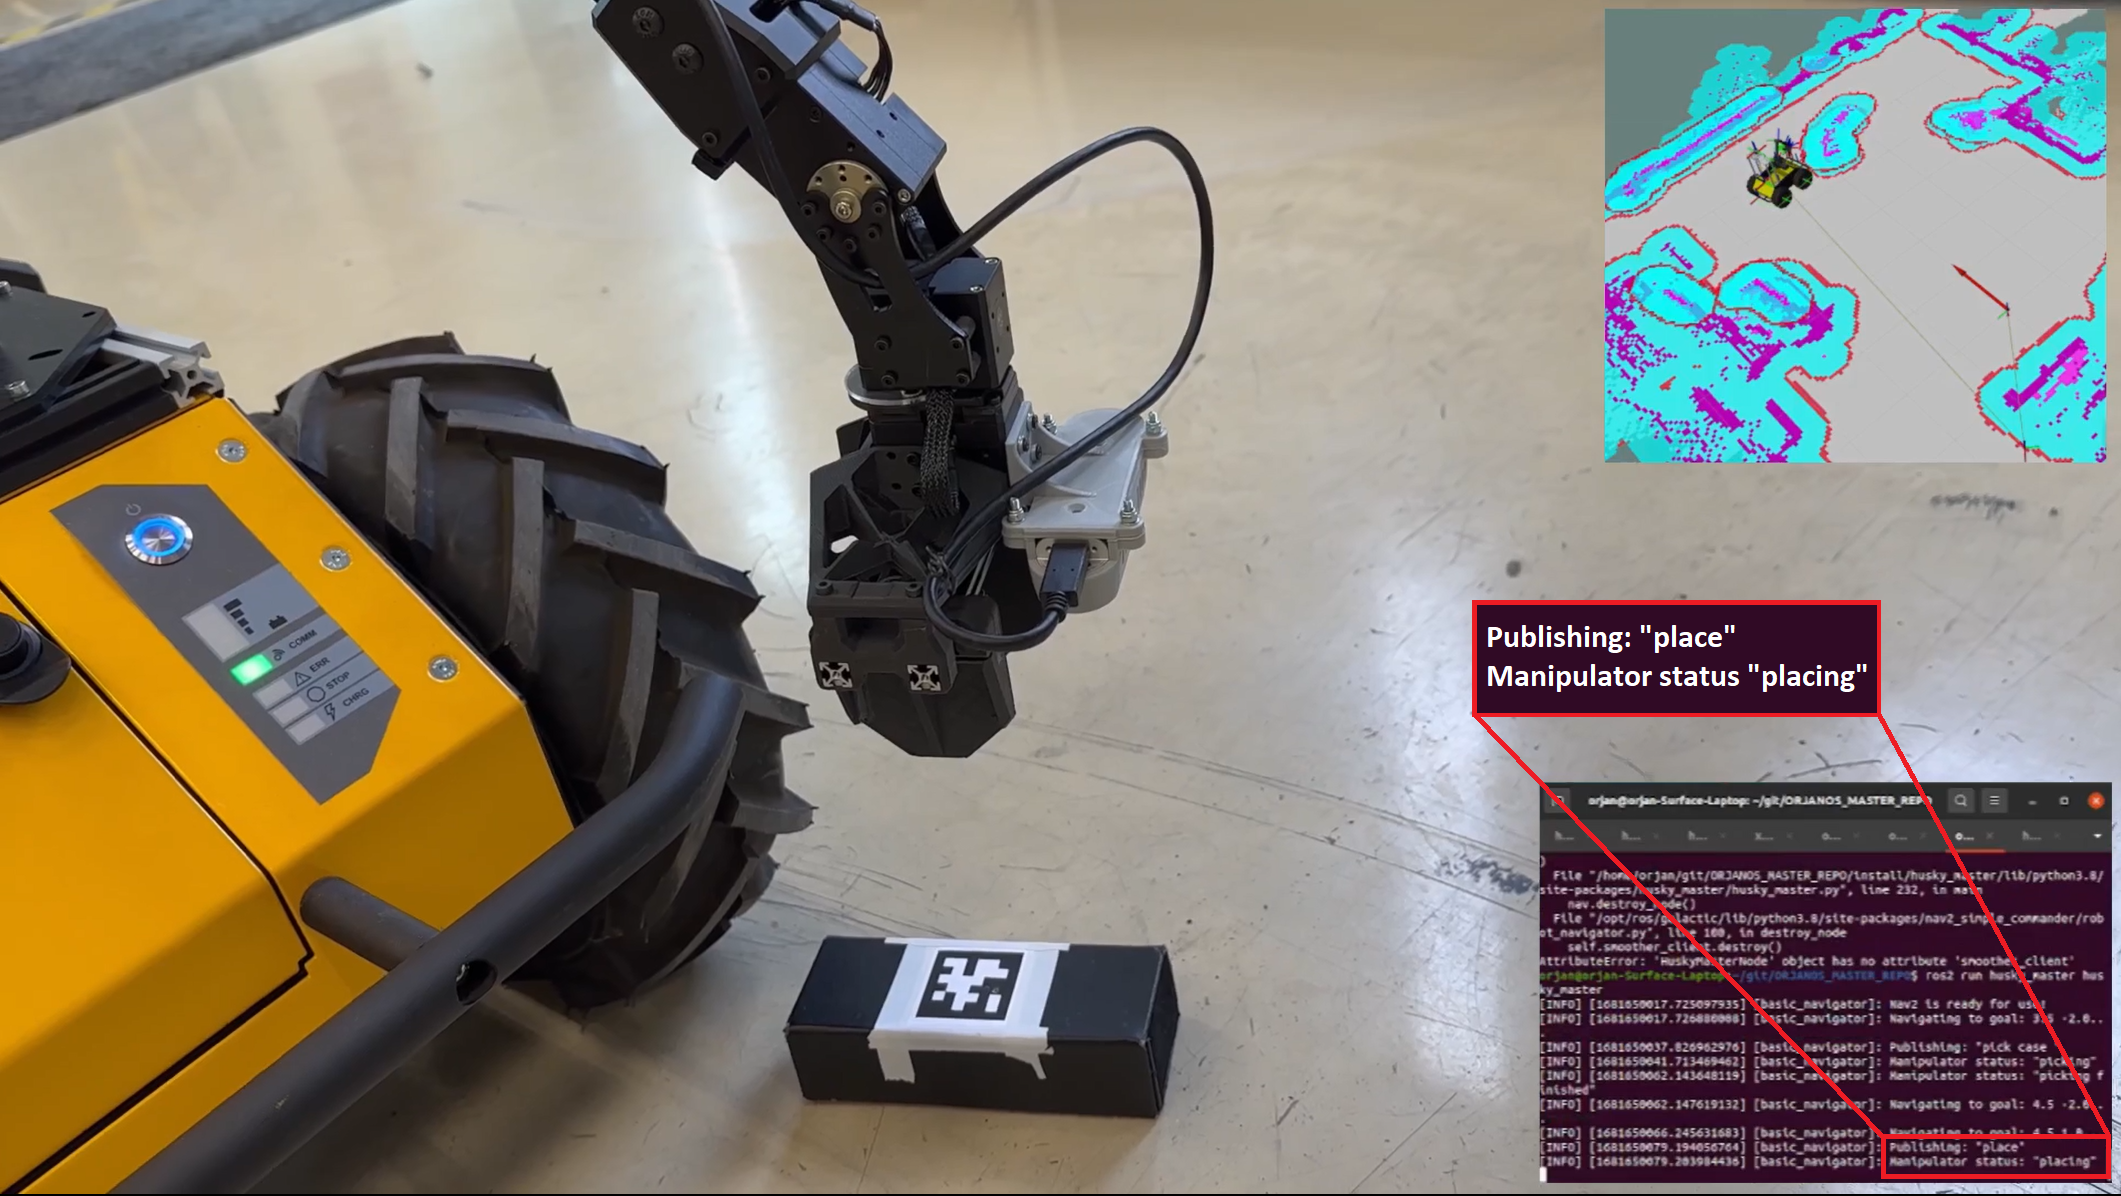
\includegraphics[width = 0.8\textwidth]{Figures/figHuskyFinalExperiment4.png}
  \caption{This figure illustrates the placing operation during the warehouse automation task. Notice from the map in the top left corner that the mobile robot has moved to a different location. Relevant command and feedback between the Husky Master node and Pick and Place node can be seen in the bloated terminal.}
  \label{fig:R:WA:finalExperiment4}
\end{figure}

After placing is finished, the mobile should return to it's starting position. This is illustrated in figure \ref{fig:R:WA:finalExperiment5}. There is a red arrow pointing at a coordinate frame in figure \ref{fig:R:WA:finalExperiment5}. This is the last known coordinate of the placed object. The bloated terminal section indicates that the placing operation is finished, and that the robot is moving to "0.0 0.0 ...", in other words, start position.

\begin{figure}[htp!]
  \centering
  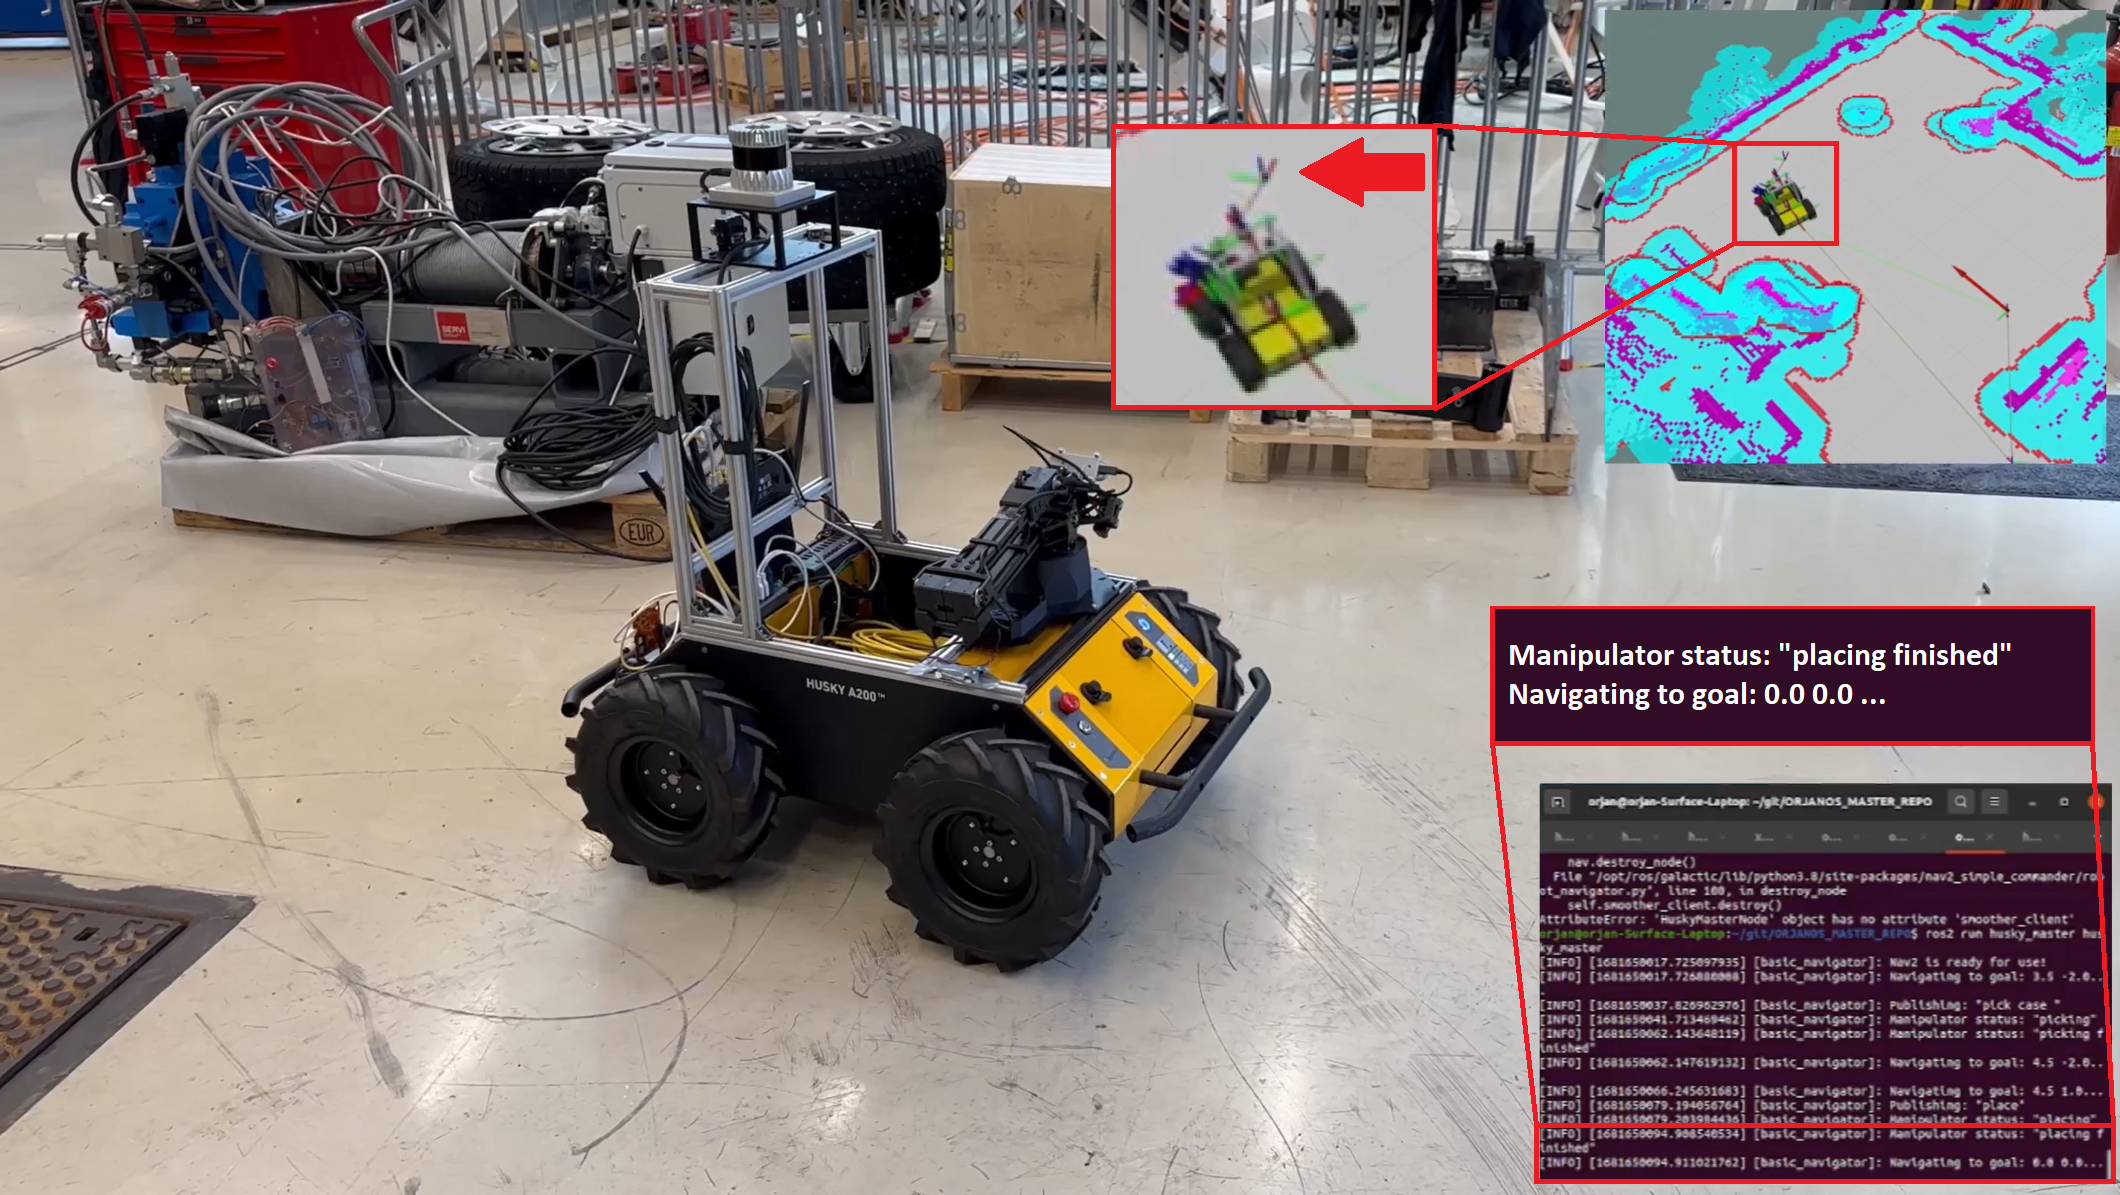
\includegraphics[width = 0.8\textwidth]{Figures/figHuskyFinalExperiment5.png}
  \caption{This figure illustrates that the mobile robot is navigating back to it's starting pose after placing the object. The bloated section from the map has a red arrow pointing at a coordinate frame behind the mobile robot. This is the last known coordinate of the placed object.}
  \label{fig:R:WA:finalExperiment5}
\end{figure}

\FloatBarrier
\subsection{Simulation Experiment}
Top-level system testing has been performed in a Gazebo simulation of the robotic system as well. This has been done by first bringing up the mobile robot simulation and the pick and place simulation. Then, a simple Gazebo environment is set up with some simple shapes, before SLAM and navigation is launched with the parameters provided in the custom ROS 2 package \lstinline{husky_group}. Finally, the top-level system is launched by running the Husky Master Node. As the computer vision system is not simulated, the detected object is represented by a static transformation from the manipulator base. Figure \ref{fig:R:WA:simTopLevel0}, \ref{fig:R:WA:simTopLevel1}, \ref{fig:R:WA:simTopLevel2} and \ref{fig:R:WA:simTopLevel3} illustrates the results of these tests. In all the four figures, the gazebo environment is illustrated in the lower right corner and a digital twin of the complete system is visualised in the top right corner. The terminal in the lower left corner gives information about progress and current status on the warehouse automation scenario.

Figure \ref{fig:R:WA:simTopLevel0} illustrates initiation of the warehouse scenario simulation experiment. The terminal in the lower right corner indicates that the husky master node is being initiated. It can also be seen that the manipulator is in it's sleep position.

\begin{figure}[htp!]
  \centering
  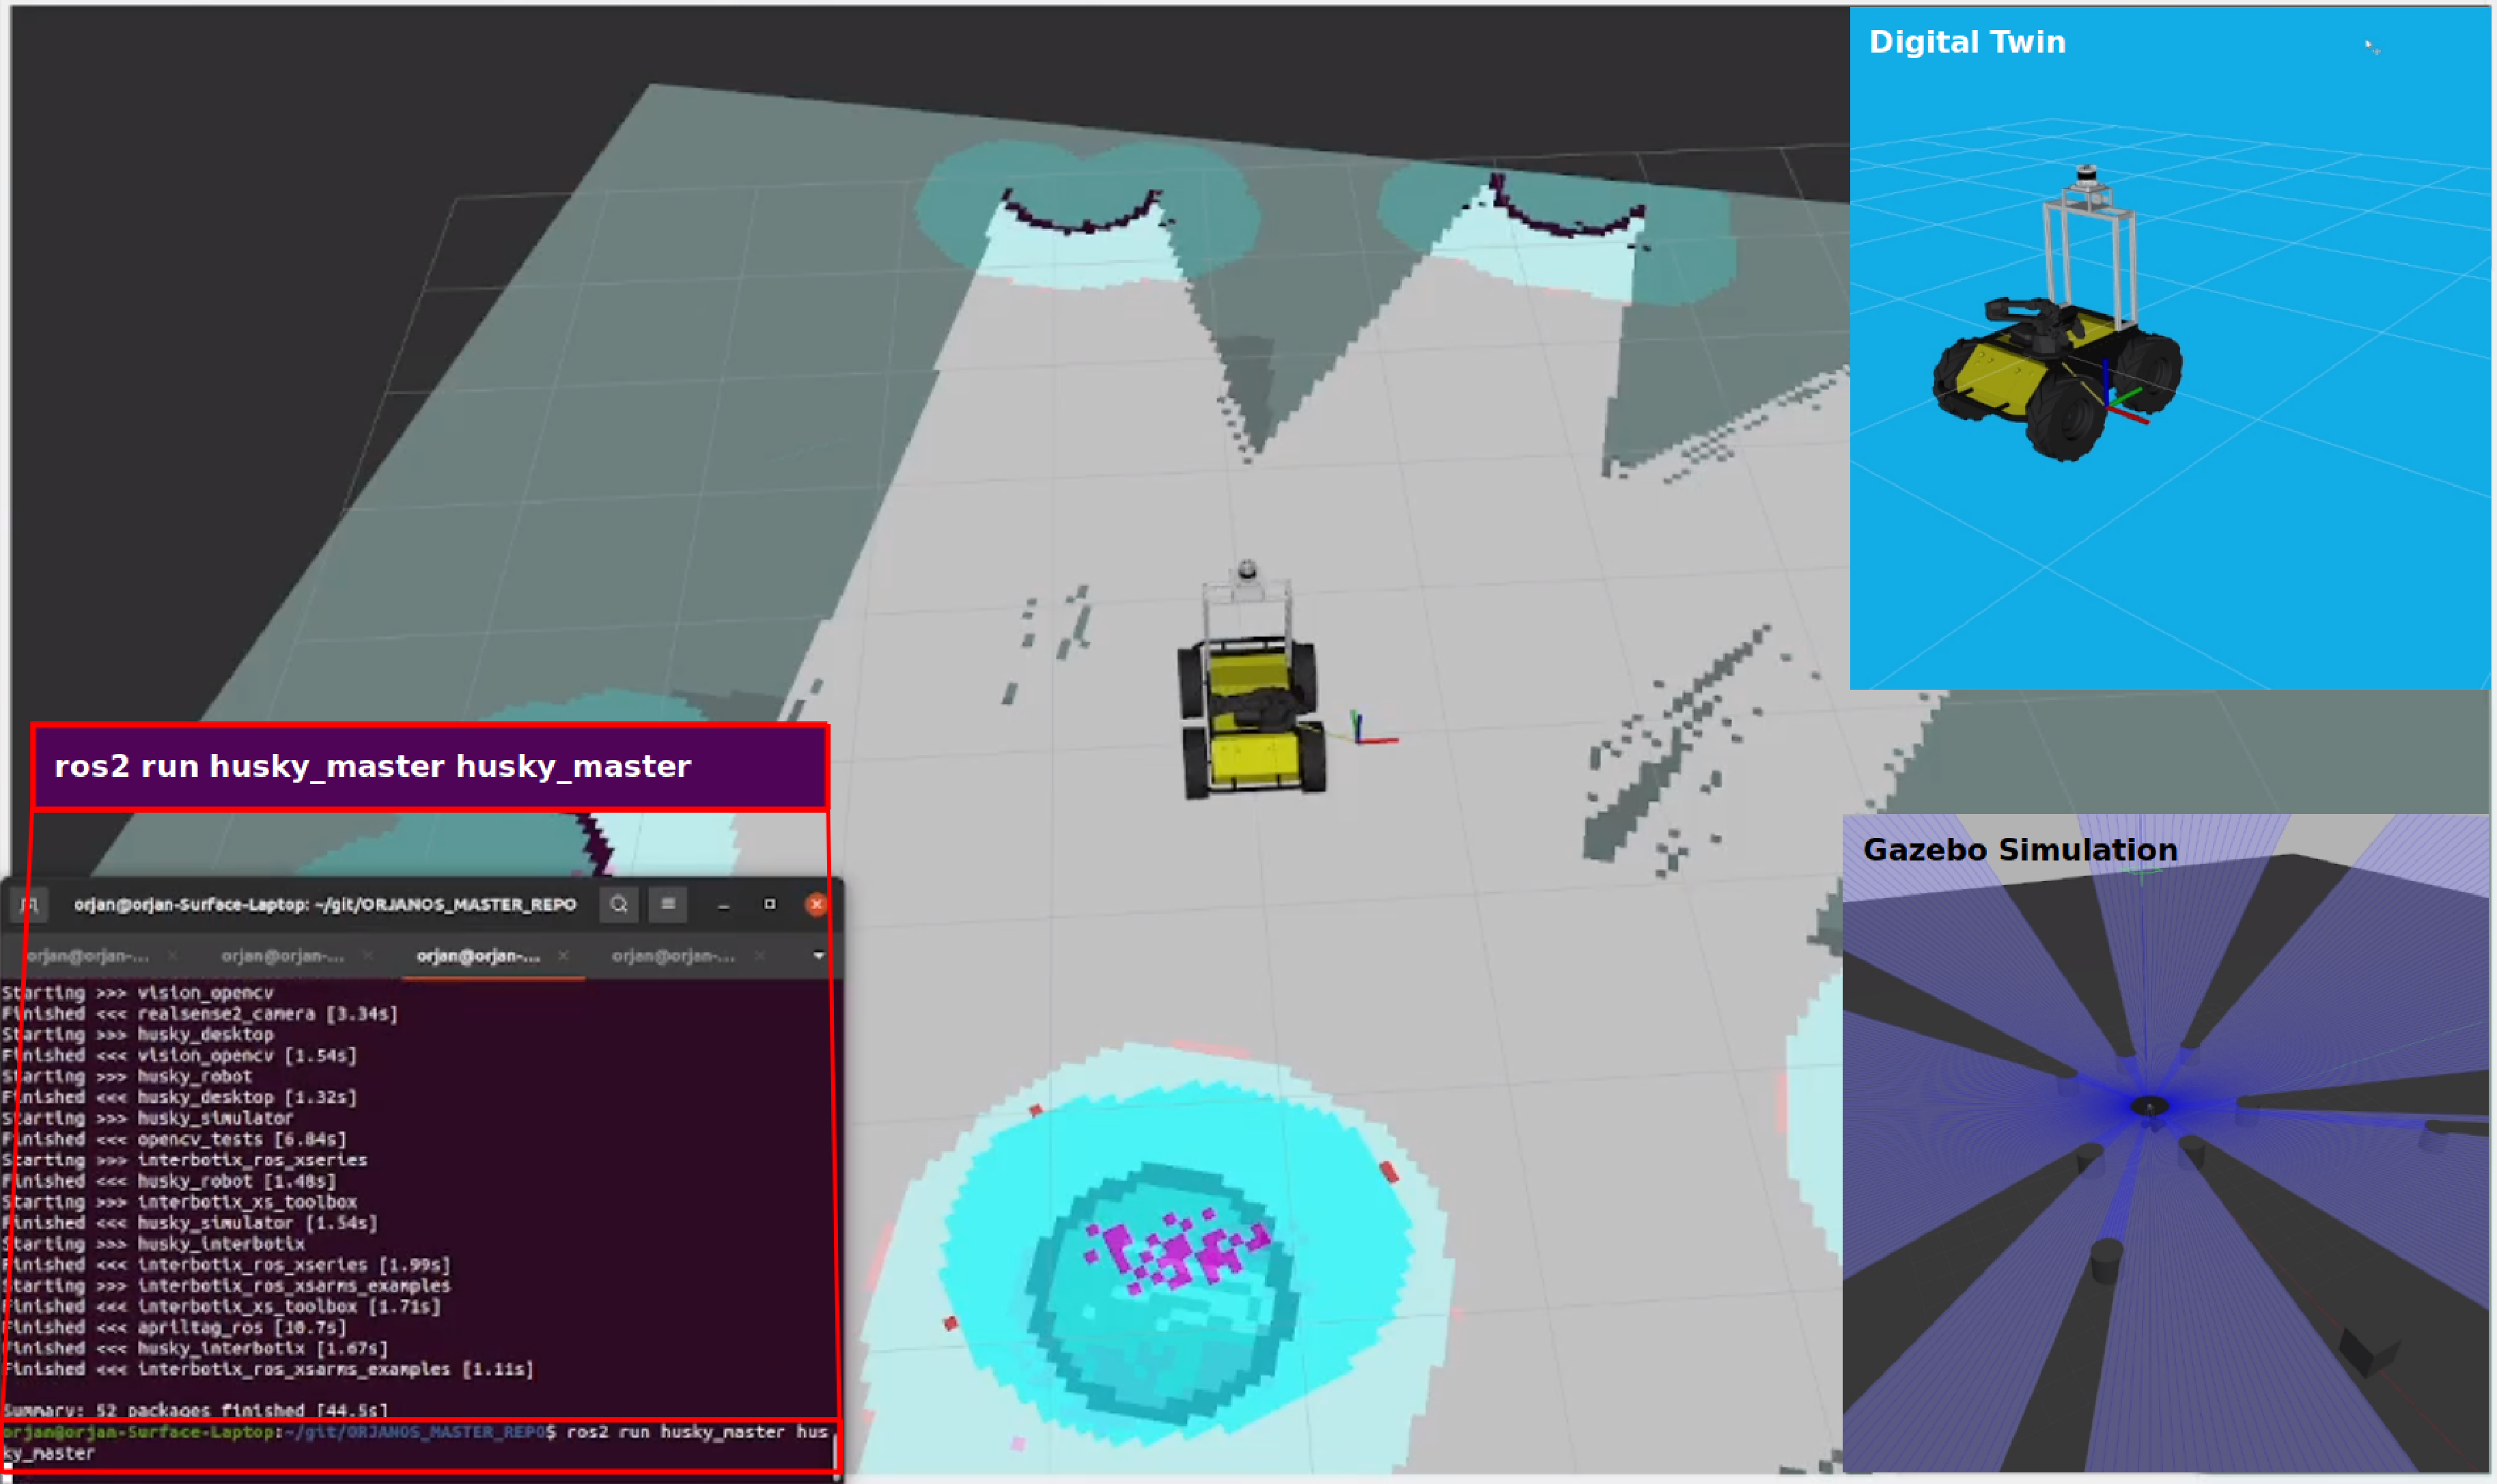
\includegraphics[width = 0.85\textwidth]{Figures/figSimTopLevel0.pdf}
  \caption{This figure illustrates initiation of top warehouse automation scenario testing in a simulation environment. \textbf{Top right:} digital twin of complete robotic system. \textbf{Lower right:} visualisation of gazebo simulation environment. \textbf{Lower left:} terminal window including bloated view of important information.}
  \label{fig:R:WA:simTopLevel0}
\end{figure}

Figure \ref{fig:R:WA:simTopLevel1} illustrates picking operation during the warehouse scenario simulation experiment. It can be seen from both the map and the Gazebo window that the mobile robot has relocated itself. The terminal window indicates that the picking operation is under way.

\begin{figure}[htp!]
  \centering
  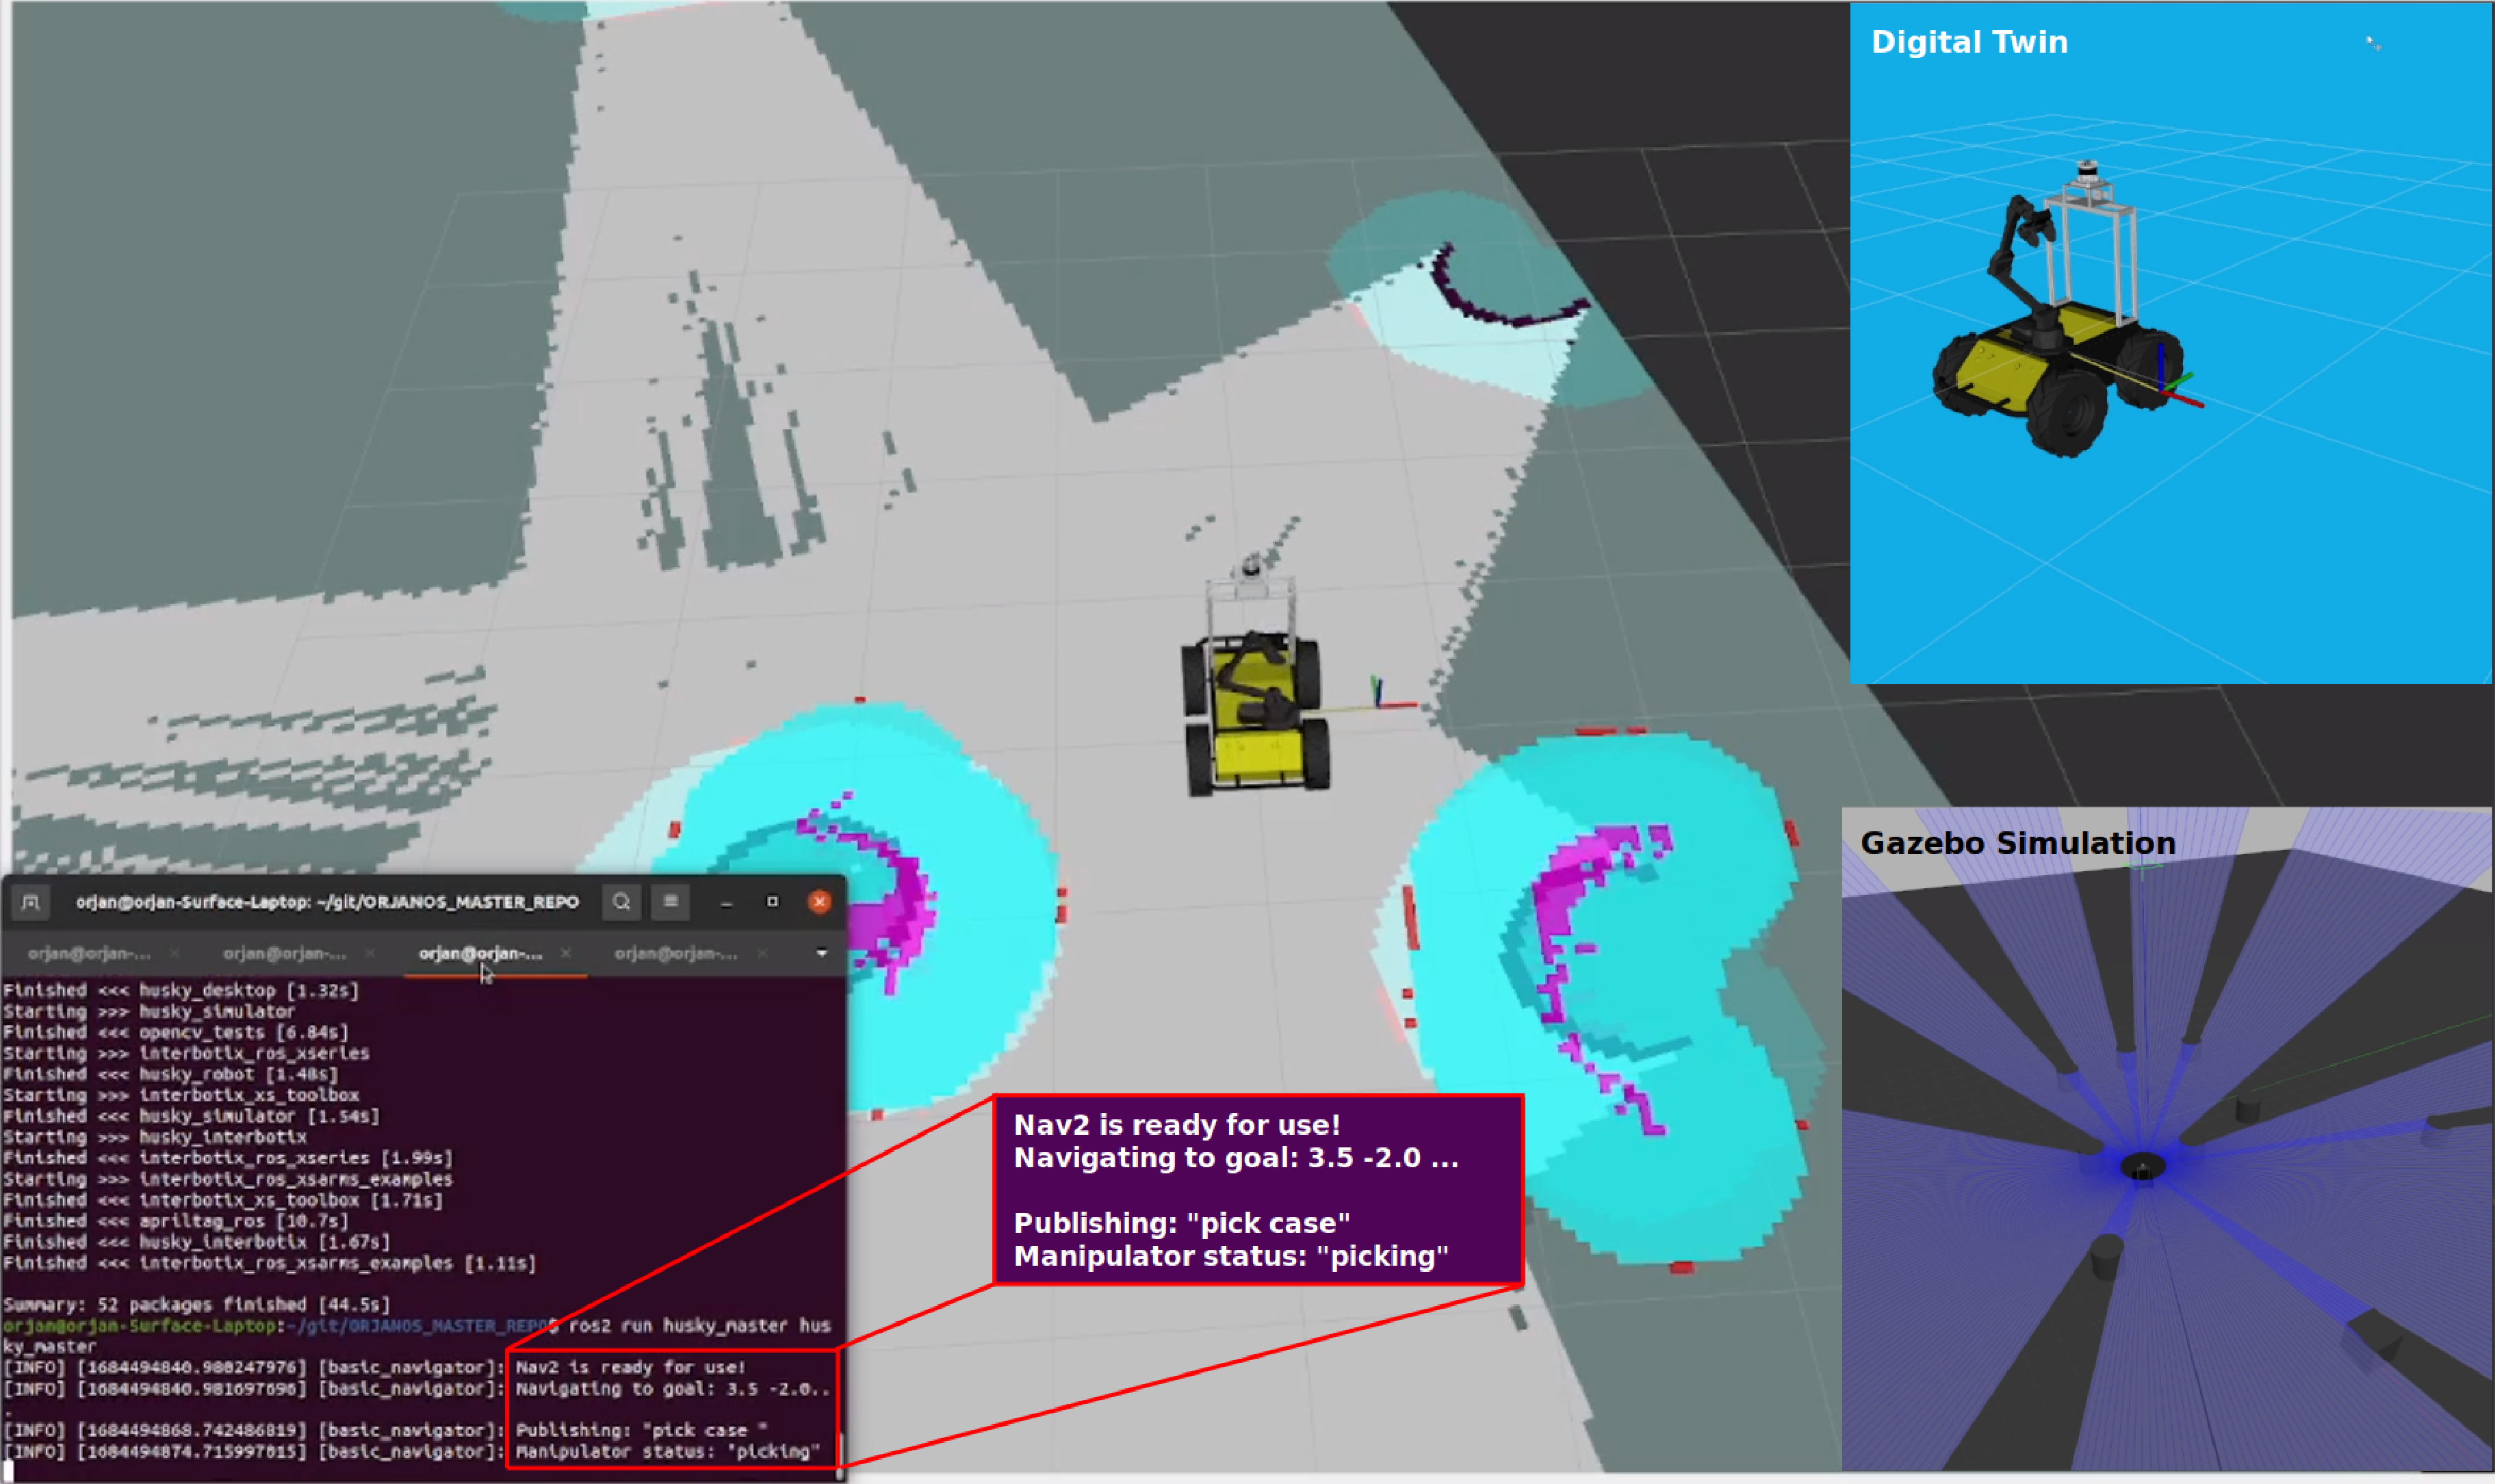
\includegraphics[width = 0.85\textwidth]{Figures/figSimTopLevel1.pdf}
  \caption{This figure illustrates picking operation during testing of top-level system on simulation of the robot in a Gazebo environment. \textbf{Top right:} digital twin of complete robotic system. \textbf{Lower right:} visualisation of gazebo simulation environment. \textbf{Lower left:} terminal window including bloated view of important information.}
  \label{fig:R:WA:simTopLevel1}
\end{figure}

Placing operation is illustrated in figure \ref{fig:R:WA:simTopLevel2}. Again, it can be seen from the map and the Gazebo window that the robot has relocated itself. The terminal confirms that the placing operation is being performed.

\begin{figure}[htp!]
  \centering
  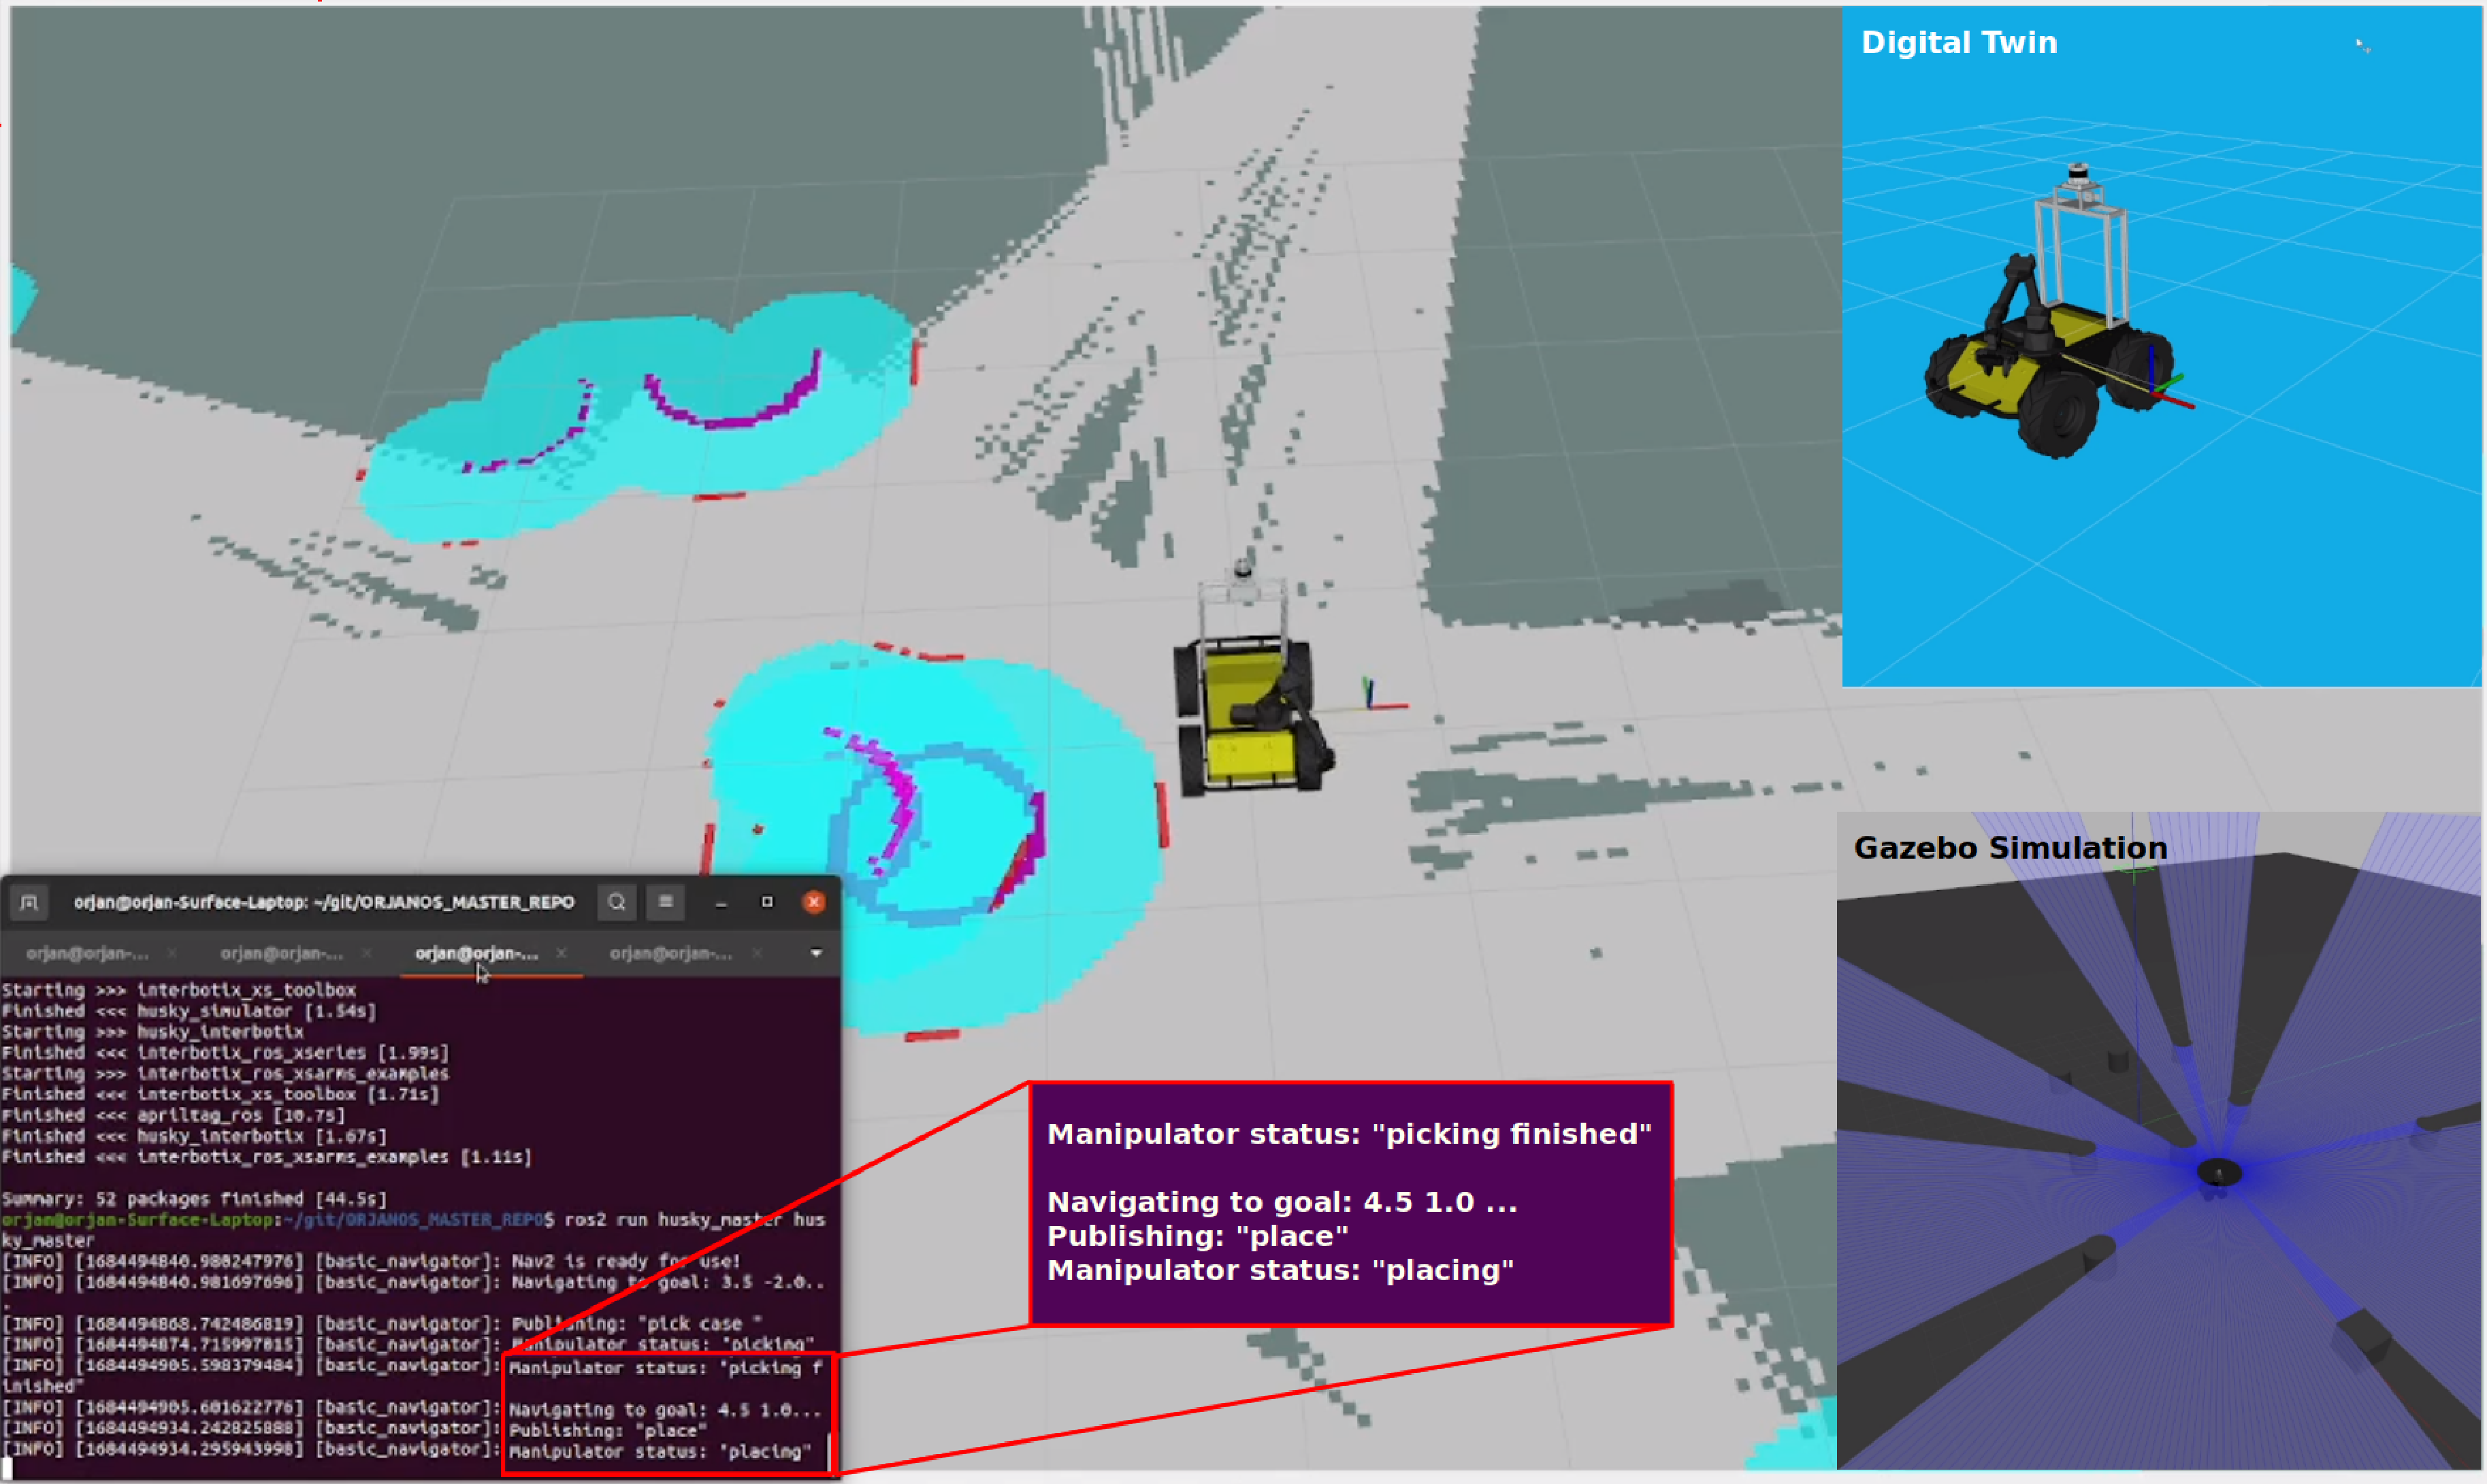
\includegraphics[width = 0.85\textwidth]{Figures/figSimTopLevel2.pdf}
  \caption{This figure illustrates placing operation during testing of top-level system on simulation of the robot in a Gazebo environment. \textbf{Top right:} digital twin of complete robotic system. \textbf{Lower right:} visualisation of gazebo simulation environment. \textbf{Lower left:} terminal window including bloated view of important information.}
  \label{fig:R:WA:simTopLevel2}
\end{figure}

Figure \ref{fig:R:WA:simTopLevel3} shows the robotic system at it's final pose. It can be seen in the gazebo window that the final pose is not the same as the start pose shown in figure \ref{fig:R:WA:simTopLevel0}. Looking at the terminal, the node reports that the UGV has reached home and is shutting down.

\begin{figure}[htp!]
  \centering
  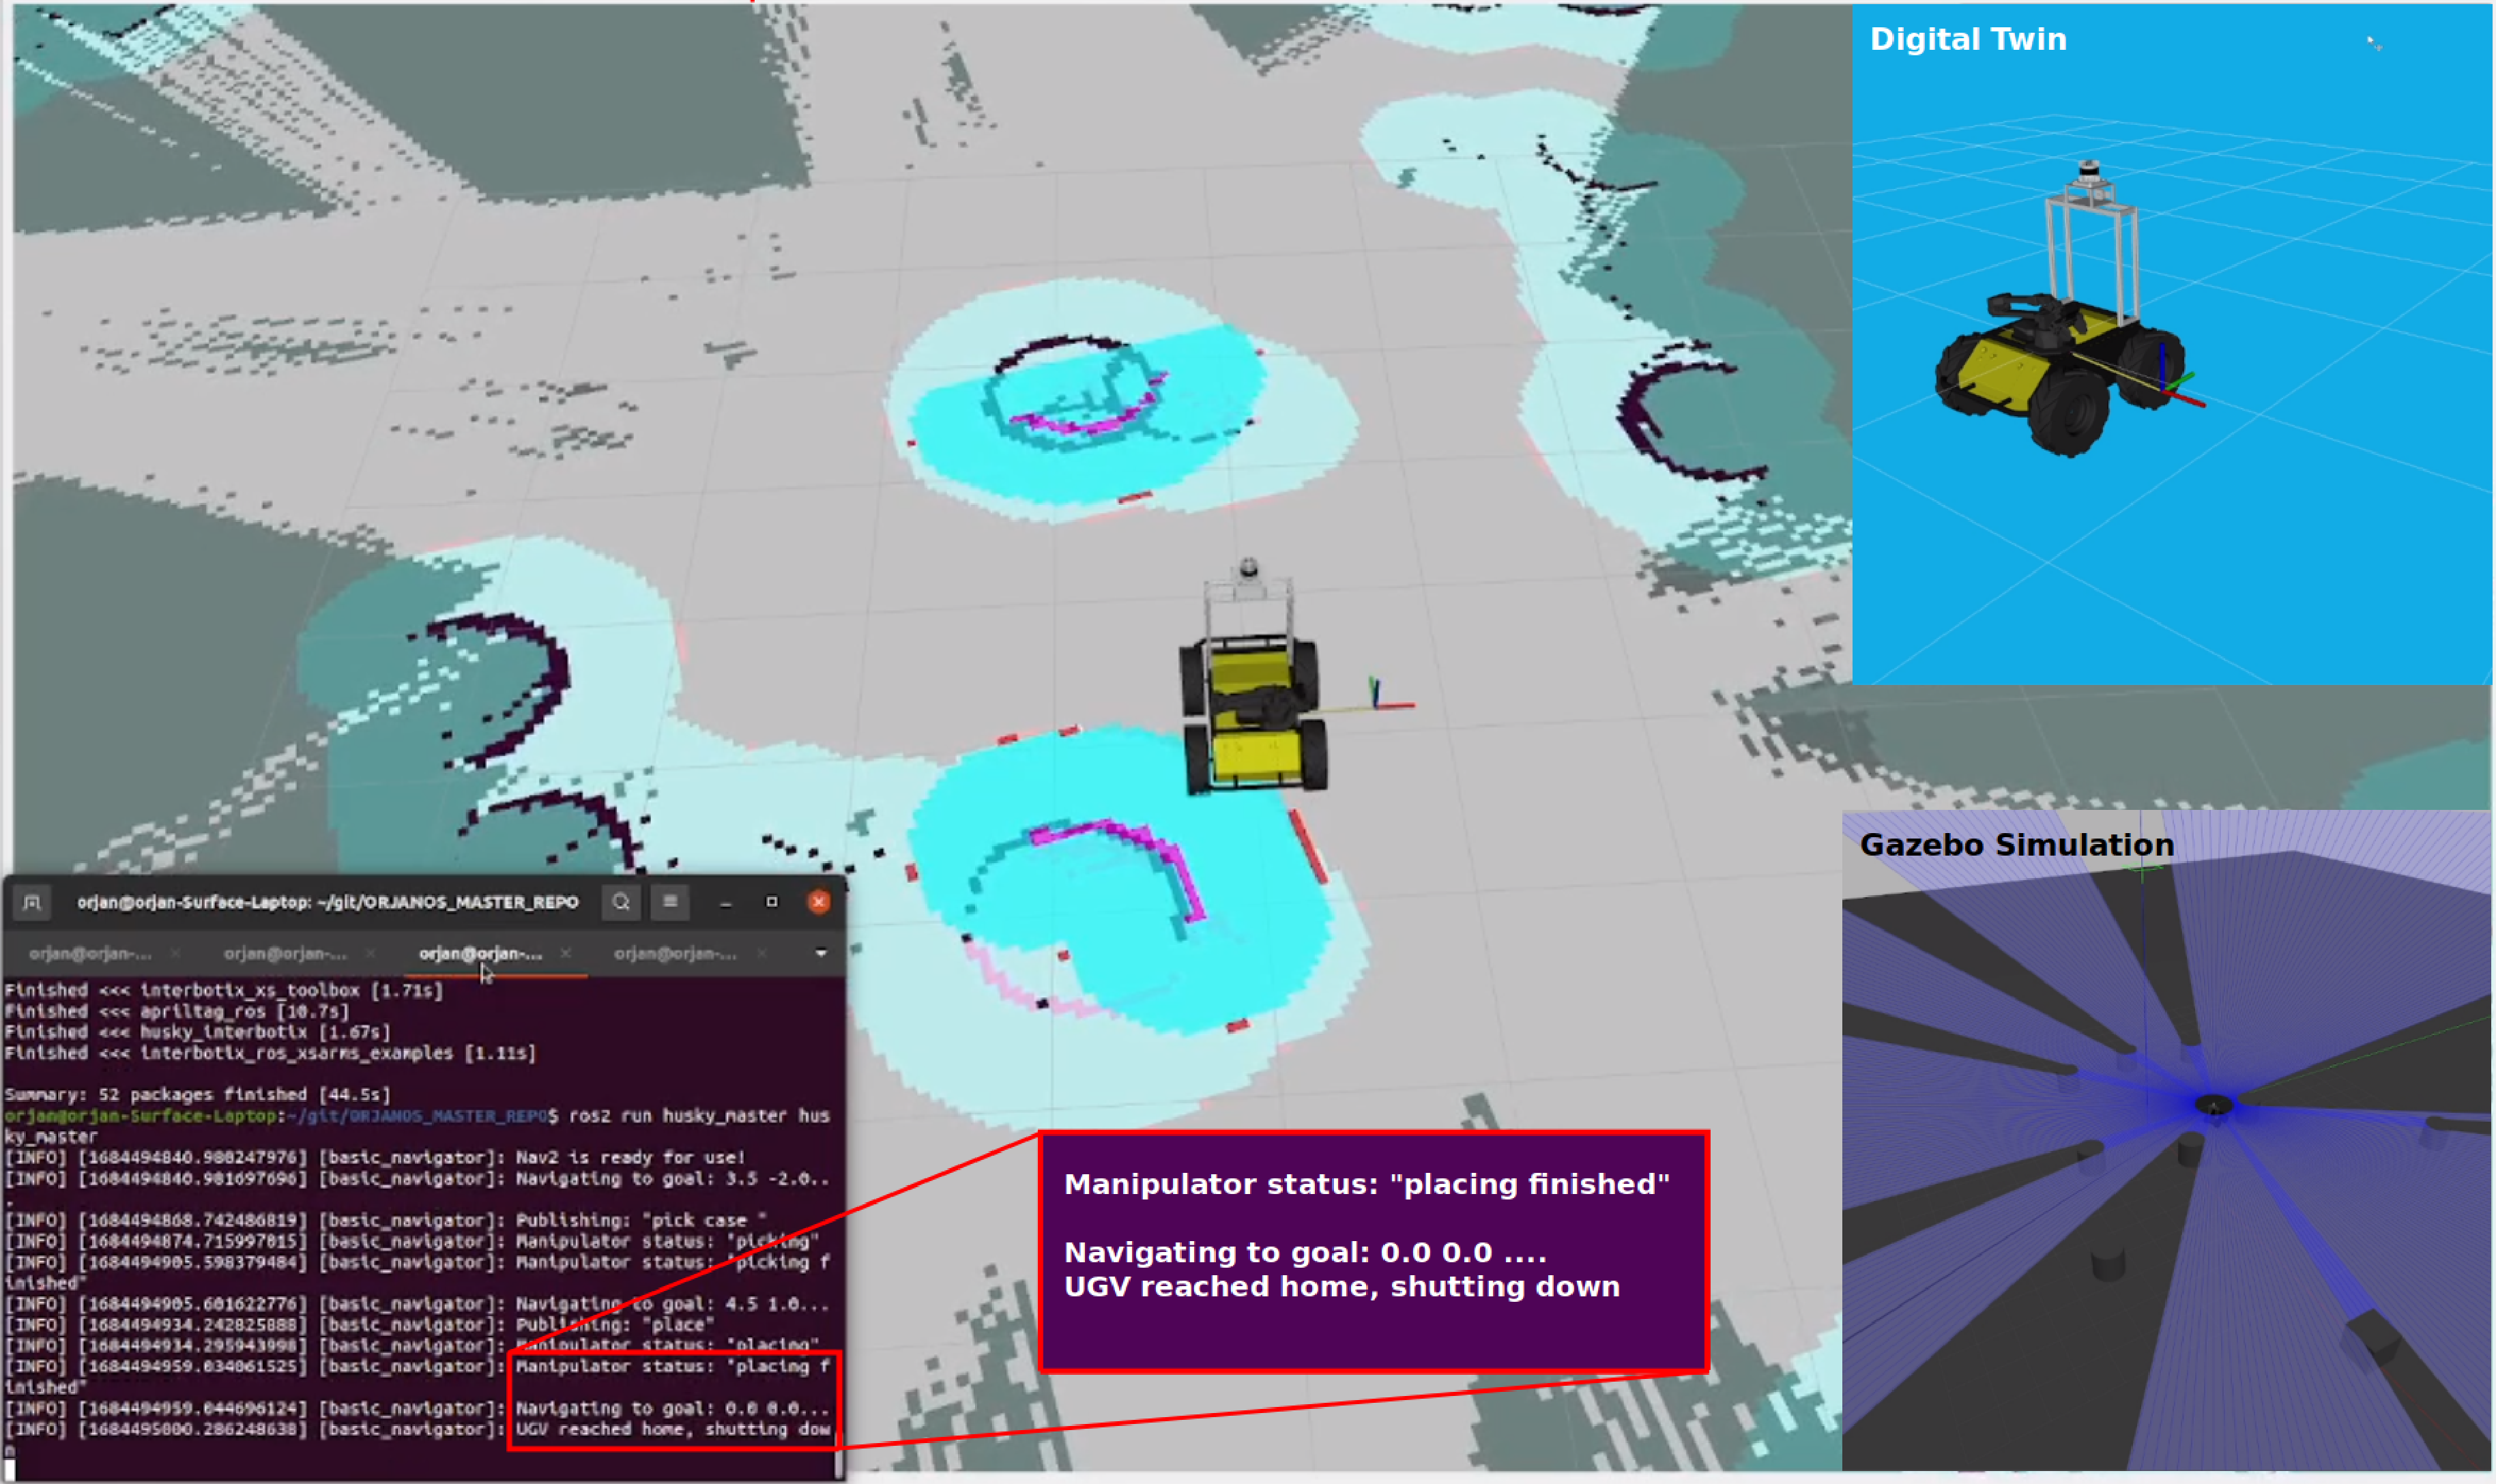
\includegraphics[width = 0.85\textwidth]{Figures/figSimTopLevel3.pdf}
  \caption{This figure illustrates testing of top-level system on simulation of the robot in a Gazebo environment. In this instance, the robot has reported that it has reached home and is shutting down. \textbf{Top right:} digital twin of complete robotic system. \textbf{Lower right:} visualisation of gazebo simulation environment. \textbf{Lower left:} terminal window including bloated view of important information.}
  \label{fig:R:WA:simTopLevel3}
\end{figure}

\FloatBarrier
\subsection{TurtleBot3 Simulation Experiment}
To test the flexibility of the top-level system for other mobile robotic platforms, the top-level system was tested together with a TurtleBot3 (popular differential drive robot for ROS and ROS 2) simulation and a virtual VX300 manipulator arm. The test is performed by launching a standard TurtleBot3 navigation simulation provided by NAV2, before launching a virtual Interbotix VX300 manipulator. The Husky Master Node is then launched to orchestrate the sequence. As there are no vision system, the detected object pose is simulated with a static transformation from the manipulators base. Figure \ref{fig:R:WA:simTBTopLevel2} provides an illustration of this test, where it can be seen that similar messages as the ones from the physical test is being displayed in the terminal window. A video of this experiment can be seen in 2x speed \href{https://youtu.be/_Dy3rSTHWYo}{here}. 

\begin{figure}[htp!]
  \centering
  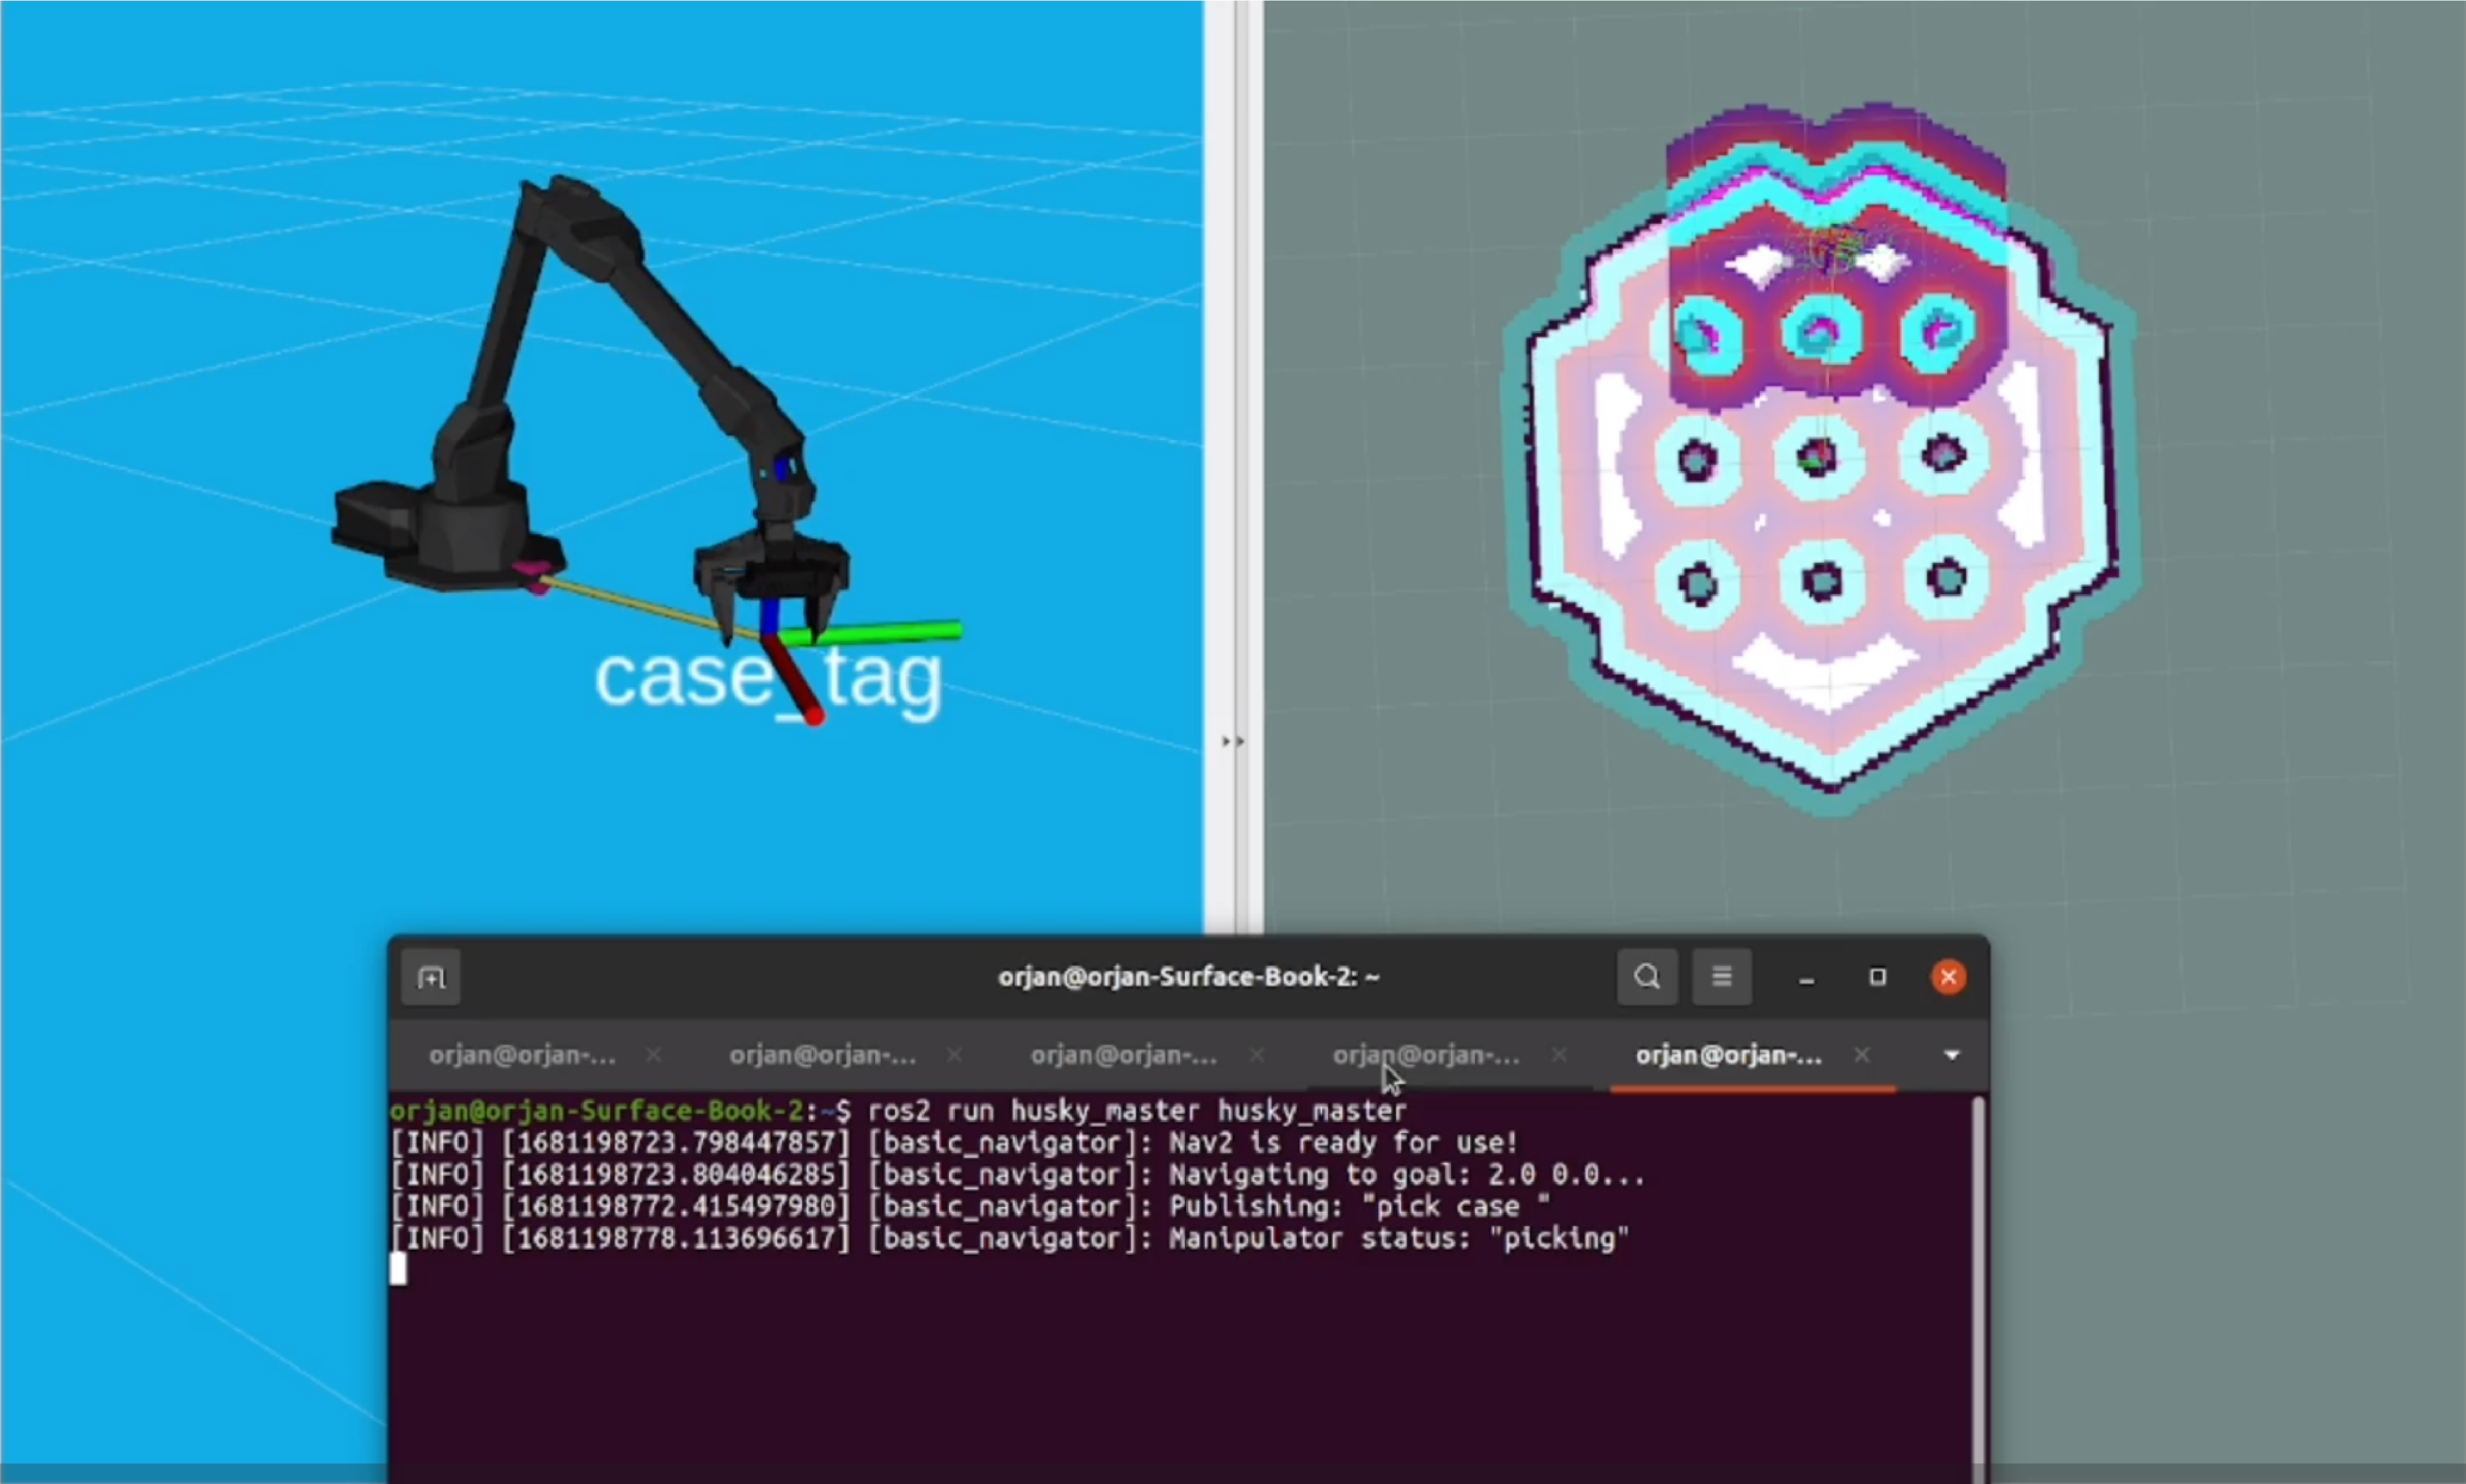
\includegraphics[width = 0.98\textwidth]{Figures/figSimTBTopLevel2.pdf}
  \caption{This figure illustrates picking operation during testing of top-level system on TurtleBot3 simulation. In this instance, the TurtleBot has reached the pick location and the manipulator is about to move its gripper down to the coordinate frame for picking. Relevant command and feedback between the Husky Master node and Pick and Place node can be seen in the terminal.}
  \label{fig:R:WA:simTBTopLevel2}
\end{figure}





%aj \section{experiment}
% write about different environment where experiment is done

% \subsection{indoor environment}

% \subsection{ware house environment}

% \section{Results}
% write that algorithms in ch 3.. was implemented to get the results with accuracy and precision, error ...

% KPI for each of functionality - show that it could navigate without collision, localize and estimate the pose of object with error xxx, pick it and place it at predefined location with error xxx

% \section{Pick and Place}



% \section{Autonomous Navigation}
% Bad kinematic design on Husky

% \section{Tag Detection}
% Worked like a charm

% \section{Pick and Place}
% Small and weak manipulator

% \section{Husky Master}
%  Unpolished Algorithm

%  \section{Husky Pick and Place}
%  Unpolished algorithm
%  Not general
%  not ideal launch file
 
%  Two methods for picking were discussed. Both of these places restrictions on the pose/shape of the objects t be picked. One method of picking bases itself on picking the objects from the side. That is, the manipulator moves in from the side of the object when gripping it. This 

%  \section{Scene Geometry Publisher}
%  Not ideal launch file
%  General design, but not general launch

 %Conclusion and Discussion
\chapter{Discussion}\label{sec:Discussion}

% During the course of this project, an autonomous UGV for warehouse pick and place application was set up. Necessary mechanical modifications were done to the UGV platform in order to accommodate extra sensors and a robotic manipulator. Then, sensors and algorithms were configured to build a demonstration of how a warehouse application system could work with an autonomous UGV. Testing was then done separately on both the the autonomous navigation system and the pick and place system. Finally, the entire pipeline was tested, where autonomous navigation, machine vision and robot manipulation works together to achieve a warehouse automation task.

\section{Hardware}\label{D:Hardware}


\subsection{Manipulator} \label{sec:D:H:Manipulator}
The mounting position of the manipulator, explained in section \ref{sec:M:H:P&PH:Manipulator}, is practical in terms of packaging and keeping the manipulator within the confinements of the UGV while not in use. Nevertheless, the limited reach of the chosen manipulator resulted in a relatively small workspace outside the bounding box of the UGV. For example, the manipulator was unable to reach the ground, meaning that objects either has to be placed on an elevated surface, or the object has to be tall enough to be picked. This is unwanted as it places a higher demand on the accuracy of the autonomous navigation system. Additionally the limited reach of the manipulator results in less flexibility in therms of object placement at pick location.
Another consideration regarding the manipulator, is the absence of brakes of any kind in the manipulator's joints. This means that the servo motors constantly has to output a torque to hold a manipulator pose. One side effect of this is unnecessary power drainage, another is the fact that there are no safety mechanisms in place in case of power cut-off or sudden control system failure. In the case of a power cut-off or sudden control system failure, the manipulator could fall uncontrollably and possibly damage itself and/or its environment.

\subsection{Manipulator Mounted Camera}\label{D:H:ManipulatorMountedCamera}
For the manipulator mounted camera, it is important that the pose of the camera is accurately defined and that the physical camera is fixed at the defined pose. The pose of the camera bracket is defined based on CAD measurements and can be assumed to be defined correctly. However, the pose of the camera relative to the bracket might not be accurately defined as this position was not thoroughly verified. 
The camera bracket described in section \ref{sec:M:H:P&PH:ManipulatorMountedCamera} proved to be successful at rigidly mounting the camera to the manipulator. However, inaccuracies in mounting pose relative to defined pose can not be ruled out due to possible slack in hole patterns at mounting flange.

\section{Autonomous Navigation} \label{sec:D:AutonomousNavigaion}

\subsection{Mobile Robot} \label{sec:D:AN:MobileRobot}
The Husky A200 UGV proved to be a practical mounting platform for developers to mount the equipment of their choice. However, there are some aspects of this UGV that should be discussed. The Husky A200 is a skidding robot (explained in section \ref{sec:T:AN:MRD:SkiddingRobots}), meaning that the robot will skid like a war-tank when turning. This is a major drawback when designing an autonomous robot since the skidding behaviour massively reduces the performance of the robot's odometry system. Sharp turns sometimes completely puts off the entire navigation system. 

\subsection{Perception} \label{sec:D:AN:Perception}
The Ouster OS1 LiDARs performance is affected by the high mounting location and it's relatively poor minimum range. Ouster states the minimum range of the LiDAR to be $r_{min}=0.8[m]$. This means that all objects within a range of $r_{min}$ from the sensor will not be detected.

The high mounting position creates a large blind-zone around the robot. This blind zone is illustrated in figure \ref{fig:D:AN:P:LidarShadow}, where it can be seen that a LiDAR mounted at a height $h[m]$ above the ground will cast a shadow with a radius $r[m]$ around the LiDAR. Notice that the orange box in figure \ref{fig:D:AN:P:LidarShadow} will not be detected by the LiDAR.

\begin{figure}[ht]
  \centering
  \includesvg[width = 0.5\textwidth]{Figures/figLiDAR_Shadow.drawio.svg}
  \caption{Illustration showing the blind-zone of the LiDAR based on it's mounting height, $h$. The green box represents the sensor, the red triangles represents the sensor's vertical field of view, and the orange box represents an object in the blind-zone of the sensor. $\theta$: half of vertical field of view. $r$: radius of shadow cast on ground.}
  \label{fig:D:AN:P:LidarShadow}
\end{figure}

The radius of the shadow cast by the LiDAR in figure \ref{fig:D:AN:P:LidarShadow}, can be mathematically described as follows. For a LiDAR mounted at a height $h[m]$ above ground and vertical field of view $2\theta[rad]$ the radius of the shadow cast on the ground, $r[m]$, is given as

\begin{equation} \label{eq:LidarShadow}
    r = \frac{h}{\tan{\theta}}[m].
\end{equation}

Ouster claims a vertical field of view of $45\deg$\textbf{SOURCE FOR THIS} which translates to $\theta=\frac{\pi}{8}[rad]$. Using equation \ref{eq:LidarShadow}, with a sensor height of $1.025[m]$, the radius of the shadow cast becomes $2.475[m]$.

The use of the ROS2 package PointCloud to LaserScan, described in section \ref{sec:M:AN:P:PointCloudToLaserScan} is considered a success as this resulted in a 2D LaserScan that took all relevant obstacles into account. This again means that a 2D map constructed from this LaserScan will take all relevant obstacles into account.

\subsection{Navigation}\label{sec:D:AN:Navigation}
Autonomous navigation performance suffered the consequences of the skidding robot design of the Husky A200, discussed in section \ref{sec:D:AN:MobileRobot}. Although the robot would successfully navigate around the environment issues occurred during hard turns. This was especially prominent in situations where the goal position had been reached, but the robot would need to spin in order to reach the correct orientation. The robot would become disoriented from the spinning action, and since the default recovery action in NAV2 is spinning, it would end up spinning in a seemingly endless dance.

\subsubsection{Collision Avoidance}
Collision avoidance would suffer from the large LiDAR blind zones discussed in section \ref{sec:D:AN:Perception}. If, for example a wall was within the minimum range of the LiDAR, the robot would have no means of detecting the wall. This could result in the robot ramming itself into walls and trying to drive through them. Objects located too low and too close could get run over due to the mounting height. A solution to this issue is presented by Didrik Robsrud in his thesis on Radar and LiDAR sensor fusion for ROS. His thesis is running in parallel to this one, and the solution from his work is therefore not implemented into this project.

% \subsection{Object Detection \& Pick and Place}
% The tag based machine vision system was set up according to section \ref{sec:M:MRC:MachineVision}. The performance of the vision system is verified by testing the combined pick and place performance of the manipulator. Interbotix states a repeatability of 1[mm] for the manipulator\cite{interbotix_vx300}. This tells that large variations in pick accuracy can be attributed to the vision system. It should be mentioned that gripper performance also plays a factor in the pick and place accuracy, as a bad gripper would not be able to achieve consistent results.

\subsection{Custom ROS2 Packages}
The custom ROS2 packages has been built and tested around a specific robotic system. It is not likely that it will work for other types of robotic systems out of the box. 


\subsubsection{Custom Pick and Place Package}



\subsection{Warehouse Automation}
The skidding behaviour of the UGV limited the performance of the this solution in that it could struggle with some poses. This navigational problem is described in section \ref{sec:D:AN:Navigation}, and placed a constraint on the warehouse automation system. This constraint is that the goal poses (pick pose, place pose, home pose) has to be carefully selected so that the robot won't have to reorient itself too much at the goal. 

The limited reach of the manipulator, discussed in section \ref{sec:D:H:Manipulator}, combined with the rectangular footprint of the UGV could cause issues. If the robot decides to do sharp turns at pick or place pose, there are chances of collision with objects.

The "Husky Master" ROS2 node that orchestrates the different behaviours of the system seemed to work as intended. The complete operation where the robot moves to a pick location, picks an object using MV, moves to a place location, places the object and moves back home was performed twice in a row with success. However, the test was preformed with goal poses that took the constraints of the navigation system and the manipulator into account.
\chapter{Conclusions}
The main goal of this thesis has been to modify an existing autonomous mobile robotic system in order to give it capabilities to preform warehouse automation tasks. Additionally, the system should be modular and easy to adapt for future students and researchers. To validate the solution, a warehouse automation scenario has been defined as a benchmark task that the system should be able to perform. 

The solution can be divided into three main categories, autonomous navigation, pick and place, and top-level. Autonomous navigation is tasked with providing robust mobile robot navigation in a warehouse environment. Pick and place is tasked with giving robust pick and place operations including computer vision-based object detection and pose estimation for picking. Top-level is tasked with orchestrating the two other parts of the solutions in order to complete the benchmark task described by the test scenario.

Although the existing mobile robot had autonomous navigation capabilities, modifications have been made to the system in order to accommodate other systems. These changes include addition of an accessory mounting frame, and merging of navigational algorithms to another Robot Operating System 2 (ROS 2) distribution. Additionally, more sensor information in the form of Inertial Measurement Unit (IMU) data is passed to the system in order to help improve performance. Nevertheless, the performance of the navigational system suffers from an inherently inaccurate locomotion mechanism in the mobile robot provided for this thesis. Sharp turns have the possibility of completely confusing the entire autonomous navigation system. The extra IMU data might have helped with this issue, but the positive effects of this modification are uncertain.

The Pick and place solution consists of a robotic manipulator, a computer vision system and ROS 2 packages developed during this project. The computer vision system is based on fiducial tag-detection using AprilTag. The chosen manipulator is a 5-degrees of freedom (DOF) manipulator by Interbotix called VX300. In order to interface the manipulator with the top-level system, a ROS 2 package that listens for simple commands, moves the manipulator based on them, and provides simple operational feedback was developed. Additionally, a ROS 2 package that encapsulates the mobile robot in collision objects, to avoid manipulator colliding with the mobile robot is made.

The fiducial tag-based computer vision system proved to give seemingly robust object detection and repeatable pose estimation, but poorly defined vision camera placement (external calibration) seemed to result in poor pose definition. No measurements were made to verify it's accuracy or repeatability. The chosen robotic manipulator gave poor performance in terms of working payload and reach. Measurements in pick and place accuracy were not made, as the computer vision system would need more adjustments. However, the manipulator was able to pick detected objects if the reported pose estimation was accurate enough.

The top-level system was tested on a physical test setup of the system, a simulated test setup of the system as well as a simulation of a TurtleBot3, which is a popular mobile robot for development and educational use. In all tests, the system was able to orchestrate the defined warehouse automation scenario. For the first two tests, some changes to the goal-pose commands sent to the navigation system was made in order to overcome issues related to navigation and limited manipulator reach. Other than this, the top-level system proved to work with various mobile robotic systems without modifications. It is worth noticing that the top-level system is more specific in terms of manipulator.

Overall, it can be concluded that this project was successful at retrofitting the provided mobile robotic system to be able to perform warehouse automation tasks. Although the solution lacks robustness, accuracy and flexibility, the solution can be seen as a proof of concept that can be further improved with future works.


\chapter{Future Work}

%\chapter{Examples}
This template is meant as an example
of how a technical report can be
structured. Discuss the table of content and the names of the chapters with the
group members and supervisor to suit your specific report.\\

\section{Some \LaTeX{} Examples}

\subsection{Using the Bibliography}

This is an example of how to use the bibliography and citations. Cite to Einstein \cite{einstein}, or something else \cite{dirac}.\\


\subsection{Writing Mathematics}

This is some examples of how to write math in \LaTeX.

\begin{equation}
    y(x) = \frac{\sin x}{e^x}
    \label{eq:label1}
\end{equation}

We can refer to the equation by using the label, like this: eq \ref{eq:label1}.\\

We can choose whether to number the equation or not:
\begin{equation*}
    y(x) = \frac{\sin x}{e^x}
\end{equation*}

Lastly, we can write inline math: $y = a \cdot x + b$ 

\subsection{Programming Code}

Inline MATLAB code: \mcode{variabel = max(input)}\\

MATLAB code in section:
\begin{lstlisting}
for i = 1 : 10
% Skriv kode her
end
\end{lstlisting}


\newpage

\subsection{Inserting Tables}

\begin{table}[H]
    \centering
    \begin{tabular}{c|c}
        Variable    &   Value   \\
        \hline
         $\theta$   &   10      \\
         $\omega$   &   40 
    \end{tabular}
    \caption{The table Caption}
    \label{tab:label1}
\end{table}

This table can be referred to by using the label, like this: table \ref{tab:label1}.


\subsection{Including figures}

\begin{figure}[H]
    \centering
    
\includegraphics[width = 0.7\textwidth]{Figures/Frontpage/forside_master_nor.pdf}
    \caption{The figure Caption}
    \label{fig:label1}
\end{figure}

This figure can be referred to by using the label, like this: figure \ref{fig:label1}.


\subsection{Multicolumn}

\begin{minipage}{0.45\textwidth}

    \vspace{-4cm}
    Text to describe for example a photo. Here we can write really long sentences just to prove the concept of the minipage, which is that the text will follow the width of the minipage that we have specified. In this case it was 45 \% of the total textwidth, with a small spacing in between, using the command "hspace". If we would like the text to start further up in the minipace, we can use the command "vspace" in front of the text, to shift it vertically.

\end{minipage}
\hspace{0.05\textwidth}
\begin{minipage}{0.45\textwidth}
 
    
\includegraphics[width = \textwidth]{Figures/Frontpage/forside_bachelor_nor.pdf}

\end{minipage}


\printbibliography[
heading=bibintoc,
title={Bibliography}
]

\appendix

\chapter{Datasheet A}

\end{document}

